\documentclass{article}

\usepackage[T1]{fontenc}
\usepackage{microtype}
\usepackage{graphicx}
\usepackage{booktabs}
\usepackage{tabularx}
\usepackage{longtable}
\usepackage{enumitem}
\usepackage{amsmath,amssymb}
\usepackage{xcolor}
\usepackage{tikz}
\usepackage{hyperref}
\usepackage{algorithm}
\usepackage{algorithmic}
\usepackage{mlsys2025}
\makeatletter\g@addto@macro\UrlBreaks{\do\-}\makeatother
\emergencystretch=2em
\usetikzlibrary{arrows.meta,positioning,shapes.misc,fit,backgrounds}

% ---------------------------------------------------------------- names
\newcommand{\capevolve}{\textsc{CapEvolve}}
% Rollout budget N and matched checkpoint N* (not B, which would clash with Suite B).
\newcommand{\budget}{\ensuremath{N}}
\newcommand{\ckpt}{\ensuremath{N^\star}}
\newcommand{\artifact}{a}
\newcommand{\Dopt}{\mathcal{D}_{\mathrm{opt}}}
\newcommand{\Dsel}{\mathcal{D}_{\mathrm{sel}}}
\newcommand{\Dfin}{\mathcal{D}_{\mathrm{fin}}}
\newcommand{\rbar}{\bar r}
\newcommand{\SE}{\mathrm{SE}}
\newcommand{\tautwo}{$\tau^2$-bench}
\providecommand{\RETURN}{\STATE \textbf{return} }

% ------------------------------------------------- draft / evidence machinery
% \draftmodetrue  -> placeholders and evidence gaps are flagged in the PDF.
% \draftmodefalse -> camera-ready. A surviving \pend prints [[PEND]] so that
%                    scripts/check_paper.py fails the build.
\newif\ifdraftmode
\draftmodetrue

% In-progress real value, expected to move before the final run.
\newcommand{\prov}[1]{\ifdraftmode\textcolor{orange!85!black}{#1}\else#1\fi}
% Evidence gap that must be closed before submission.
\newcommand{\needs}[1]{\ifdraftmode\textcolor{red!80!black}{\textsuperscript{$\triangle$}\footnote{\textcolor{red!80!black}{\textbf{EVIDENCE NEEDED:} #1}}}\else\fi}
% Inline editorial note.
\newcommand{\note}[1]{\ifdraftmode\textcolor{blue!65!black}{[#1]}\else\fi}
% Mock placeholder for a result that does not exist yet.
\newcommand{\pend}[1]{\ifdraftmode\textcolor{red!80!black}{#1\textsuperscript{\dag}}\else[[PEND]]\fi}

% Real values (derive_numbers.py) and mock values (mock_numbers.py).
% GENERATED by scripts/derive_numbers.py. Do not edit by hand.
% Real values read from repo files. In-progress values are wrapped in \prov.
\newcommand{\costACalls}{\prov{27\,760}}
\newcommand{\costATokensM}{\prov{183}}
\newcommand{\costBCalls}{\prov{79\,322}}
\newcommand{\costBTokensM}{\prov{377}}
\newcommand{\costCCalls}{\prov{9\,455}}
\newcommand{\costCTokensM}{\prov{45}}
\newcommand{\costCalls}{\prov{118\,556}}
\newcommand{\costNonRitsM}{\prov{25.9}}
\newcommand{\costRitsM}{\prov{591}}
\newcommand{\costTokensM}{\prov{617}}
\newcommand{\costUsdProxy}{\prov{82}}
\newcommand{\goldOptimizerRuns}{6}
\newcommand{\goldRolloutsHits}{0}
\newcommand{\goldRolloutsScanned}{2{,}049}
\newcommand{\histFormulaGoldPct}{70.5}
\newcommand{\histFormulaGoldTasks}{282}
\newcommand{\histGemmaBaseRecalc}{58.3}
\newcommand{\histGemmaBaseSaved}{43.5}
\newcommand{\histGemmaCompliancePts}{14}
\newcommand{\histGemmaDeltaRecalc}{18.7}
\newcommand{\histGemmaDeltaSaved}{33.0}
\newcommand{\histGptBaseRecalc}{77.5}
\newcommand{\histGptBaseSaved}{38.5}
\newcommand{\histGptCompliancePts}{39}
\newcommand{\histGptDeltaRecalc}{9.9}
\newcommand{\histGptDeltaSaved}{49.1}
\newcommand{\mdeFortyArtifact}{0.13}
\newcommand{\mdeFortyPipeline}{0.26}
\newcommand{\mdeHundredArtifact}{0.08}
\newcommand{\mdeTwoEightyArtifact}{0.05}
\newcommand{\mdeTwoEightyPipeline}{0.13}
\newcommand{\replayBlockedRuns}{6}
\newcommand{\replayDecisions}{96}
\newcommand{\replayFlipsUnmasked}{10}
\newcommand{\replayKtwo}{38}
\newcommand{\replayPathRuns}{16}
\newcommand{\replayRecorded}{33}
\newcommand{\replayRuns}{19}
\newcommand{\replaySurviveRuns}{10}
\newcommand{\replayUnmasked}{23}
\newcommand{\simAFalse}{0.014}
\newcommand{\simAPowerEight}{0.15}
\newcommand{\simAPowerFour}{0.03}
\newcommand{\simAPowerSix}{0.08}
\newcommand{\simAPowerTen}{0.26}
\newcommand{\simDFalse}{0.019}
\newcommand{\simDPowerEight}{0.29}
\newcommand{\simDPowerFour}{0.08}
\newcommand{\simDPowerSix}{0.16}
\newcommand{\simDPowerTen}{0.42}
\newcommand{\simKoneFalse}{0.565}
\newcommand{\simKonePowerEight}{0.45}
\newcommand{\simKonePowerFour}{0.29}
\newcommand{\simKonePowerSix}{0.37}
\newcommand{\simKonePowerTen}{0.54}
\newcommand{\simPFalse}{0.055}
\newcommand{\simPPowerEight}{0.27}
\newcommand{\simPPowerFour}{0.09}
\newcommand{\simPPowerSix}{0.17}
\newcommand{\simPPowerTen}{0.41}

% GENERATED by scripts/mock_numbers.py (seed 20261013). MOCK VALUES. Do not edit.
% Every macro is wrapped in \pend; check_paper.py must fail if any survives with \draftmodefalse.
\newcommand{\mockAaceDelta}{\pend{+5.8}}
\newcommand{\mockAaceHi}{\pend{+9.9}}
\newcommand{\mockAaceLo}{\pend{+1.8}}
\newcommand{\mockAaceMiss}{\pend{4/720}}
\newcommand{\mockAacePholm}{\pend{0.032}}
\newcommand{\mockAaceRoll}{\pend{536}}
\newcommand{\mockAaceScore}{\pend{55.8}}
\newcommand{\mockAaceTokCr}{\pend{4.2}}
\newcommand{\mockAaceTokCw}{\pend{1.0}}
\newcommand{\mockAaceTokU}{\pend{25.4}}
\newcommand{\mockAaceUsd}{\pend{87}}
\newcommand{\mockAaceWall}{\pend{21.7}}
\newcommand{\mockAaoDelta}{\pend{+3.6}}
\newcommand{\mockAaoHi}{\pend{+8.7}}
\newcommand{\mockAaoLo}{\pend{$-$1.5}}
\newcommand{\mockAaoMiss}{\pend{3/720}}
\newcommand{\mockAaoPholm}{\pend{0.738}}
\newcommand{\mockAaoRoll}{\pend{536}}
\newcommand{\mockAaoScore}{\pend{53.6}}
\newcommand{\mockAaoTokCr}{\pend{68.4}}
\newcommand{\mockAaoTokCw}{\pend{7.8}}
\newcommand{\mockAaoTokU}{\pend{19.5}}
\newcommand{\mockAaoUsd}{\pend{98}}
\newcommand{\mockAaoWall}{\pend{25.6}}
\newcommand{\mockAevoskillDelta}{\pend{+2.2}}
\newcommand{\mockAevoskillHi}{\pend{+7.2}}
\newcommand{\mockAevoskillLo}{\pend{$-$2.8}}
\newcommand{\mockAevoskillMiss}{\pend{4/720}}
\newcommand{\mockAevoskillPholm}{\pend{1.000}}
\newcommand{\mockAevoskillRoll}{\pend{538}}
\newcommand{\mockAevoskillScore}{\pend{52.2}}
\newcommand{\mockAevoskillTokCr}{\pend{87.2}}
\newcommand{\mockAevoskillTokCw}{\pend{7.2}}
\newcommand{\mockAevoskillTokU}{\pend{31.4}}
\newcommand{\mockAevoskillUsd}{\pend{146}}
\newcommand{\mockAevoskillWall}{\pend{28.7}}
\newcommand{\mockAgepaDelta}{\pend{+3.3}}
\newcommand{\mockAgepaHi}{\pend{+7.8}}
\newcommand{\mockAgepaLo}{\pend{$-$1.1}}
\newcommand{\mockAgepaMiss}{\pend{1/720}}
\newcommand{\mockAgepaPholm}{\pend{0.724}}
\newcommand{\mockAgepaRoll}{\pend{529}}
\newcommand{\mockAgepaScore}{\pend{53.3}}
\newcommand{\mockAgepaTokCr}{\pend{4.3}}
\newcommand{\mockAgepaTokCw}{\pend{0.8}}
\newcommand{\mockAgepaTokU}{\pend{28.1}}
\newcommand{\mockAgepaUsd}{\pend{86}}
\newcommand{\mockAgepaWall}{\pend{20.2}}
\newcommand{\mockAhcDelta}{\pend{+3.4}}
\newcommand{\mockAhcHi}{\pend{+8.5}}
\newcommand{\mockAhcLo}{\pend{$-$1.7}}
\newcommand{\mockAhcMiss}{\pend{5/720}}
\newcommand{\mockAhcPholm}{\pend{0.738}}
\newcommand{\mockAhcRoll}{\pend{534}}
\newcommand{\mockAhcScore}{\pend{53.4}}
\newcommand{\mockAhcTokCr}{\pend{78.6}}
\newcommand{\mockAhcTokCw}{\pend{6.3}}
\newcommand{\mockAhcTokU}{\pend{14.7}}
\newcommand{\mockAhcUsd}{\pend{76}}
\newcommand{\mockAhcWall}{\pend{24.1}}
\newcommand{\mockAmetaharnessDelta}{\pend{+1.1}}
\newcommand{\mockAmetaharnessHi}{\pend{+6.2}}
\newcommand{\mockAmetaharnessLo}{\pend{$-$4.0}}
\newcommand{\mockAmetaharnessMiss}{\pend{2/720}}
\newcommand{\mockAmetaharnessPholm}{\pend{1.000}}
\newcommand{\mockAmetaharnessRoll}{\pend{528}}
\newcommand{\mockAmetaharnessScore}{\pend{51.1}}
\newcommand{\mockAmetaharnessTokCr}{\pend{27.0}}
\newcommand{\mockAmetaharnessTokCw}{\pend{2.8}}
\newcommand{\mockAmetaharnessTokU}{\pend{43.1}}
\newcommand{\mockAmetaharnessUsd}{\pend{162}}
\newcommand{\mockAmetaharnessWall}{\pend{27.4}}
\newcommand{\mockAmiproDelta}{\pend{+5.5}}
\newcommand{\mockAmiproHi}{\pend{+10.0}}
\newcommand{\mockAmiproLo}{\pend{+1.0}}
\newcommand{\mockAmiproMiss}{\pend{4/720}}
\newcommand{\mockAmiproPholm}{\pend{0.098}}
\newcommand{\mockAmiproRoll}{\pend{532}}
\newcommand{\mockAmiproScore}{\pend{55.5}}
\newcommand{\mockAmiproTokCr}{\pend{1.1}}
\newcommand{\mockAmiproTokCw}{\pend{0.7}}
\newcommand{\mockAmiproTokU}{\pend{26.3}}
\newcommand{\mockAmiproUsd}{\pend{78}}
\newcommand{\mockAmiproWall}{\pend{27.6}}
\newcommand{\mockAoneshotDelta}{\pend{+1.9}}
\newcommand{\mockAoneshotHi}{\pend{+6.7}}
\newcommand{\mockAoneshotLo}{\pend{$-$2.9}}
\newcommand{\mockAoneshotMiss}{\pend{2/720}}
\newcommand{\mockAoneshotPholm}{\pend{1.000}}
\newcommand{\mockAoneshotRoll}{\pend{10}}
\newcommand{\mockAoneshotScore}{\pend{51.9}}
\newcommand{\mockAoneshotTokCr}{\pend{5.6}}
\newcommand{\mockAoneshotTokCw}{\pend{0.4}}
\newcommand{\mockAoneshotTokU}{\pend{18.9}}
\newcommand{\mockAoneshotUsd}{\pend{58}}
\newcommand{\mockAoneshotWall}{\pend{1.0}}
\newcommand{\mockAseedDelta}{\pend{+0.0}}
\newcommand{\mockAseedMiss}{\pend{0/240}}
\newcommand{\mockAseedRoll}{\pend{0}}
\newcommand{\mockAseedScore}{\pend{50.0}}
\newcommand{\mockAseedTokCr}{\pend{0.0}}
\newcommand{\mockAseedTokCw}{\pend{0.0}}
\newcommand{\mockAseedTokU}{\pend{0.0}}
\newcommand{\mockAseedUsd}{\pend{0}}
\newcommand{\mockAseedWall}{\pend{0.0}}
\newcommand{\mockAskilloptDelta}{\pend{+6.7}}
\newcommand{\mockAskilloptHi}{\pend{+11.4}}
\newcommand{\mockAskilloptLo}{\pend{+2.0}}
\newcommand{\mockAskilloptMiss}{\pend{6/720}}
\newcommand{\mockAskilloptPholm}{\pend{0.033}}
\newcommand{\mockAskilloptRoll}{\pend{528}}
\newcommand{\mockAskilloptScore}{\pend{56.7}}
\newcommand{\mockAskilloptTokCr}{\pend{7.6}}
\newcommand{\mockAskilloptTokCw}{\pend{0.6}}
\newcommand{\mockAskilloptTokU}{\pend{15.0}}
\newcommand{\mockAskilloptUsd}{\pend{49}}
\newcommand{\mockAskilloptWall}{\pend{22.0}}
\newcommand{\mockAtracetwoskillDelta}{\pend{+5.2}}
\newcommand{\mockAtracetwoskillHi}{\pend{+10.2}}
\newcommand{\mockAtracetwoskillLo}{\pend{+0.2}}
\newcommand{\mockAtracetwoskillMiss}{\pend{6/720}}
\newcommand{\mockAtracetwoskillPholm}{\pend{0.220}}
\newcommand{\mockAtracetwoskillRoll}{\pend{536}}
\newcommand{\mockAtracetwoskillScore}{\pend{55.2}}
\newcommand{\mockAtracetwoskillTokCr}{\pend{3.3}}
\newcommand{\mockAtracetwoskillTokCw}{\pend{0.7}}
\newcommand{\mockAtracetwoskillTokU}{\pend{14.4}}
\newcommand{\mockAtracetwoskillUsd}{\pend{49}}
\newcommand{\mockAtracetwoskillWall}{\pend{11.6}}
\newcommand{\mockAwikiskillDelta}{\pend{+5.9}}
\newcommand{\mockAwikiskillHi}{\pend{+10.8}}
\newcommand{\mockAwikiskillLo}{\pend{+1.0}}
\newcommand{\mockAwikiskillMiss}{\pend{1/720}}
\newcommand{\mockAwikiskillPholm}{\pend{0.098}}
\newcommand{\mockAwikiskillRoll}{\pend{533}}
\newcommand{\mockAwikiskillScore}{\pend{55.9}}
\newcommand{\mockAwikiskillTokCr}{\pend{0.1}}
\newcommand{\mockAwikiskillTokCw}{\pend{0.5}}
\newcommand{\mockAwikiskillTokU}{\pend{4.4}}
\newcommand{\mockAwikiskillUsd}{\pend{16}}
\newcommand{\mockAwikiskillWall}{\pend{26.7}}
\newcommand{\mockBaoDelta}{\pend{+1.8}}
\newcommand{\mockBaoHi}{\pend{+10.8}}
\newcommand{\mockBaoLo}{\pend{$-$7.2}}
\newcommand{\mockBaoMiss}{\pend{8/360}}
\newcommand{\mockBaoPholm}{\pend{1.000}}
\newcommand{\mockBaoRoll}{\pend{470}}
\newcommand{\mockBaoScore}{\pend{56.8}}
\newcommand{\mockBaoTokCr}{\pend{120.0}}
\newcommand{\mockBaoTokCw}{\pend{8.9}}
\newcommand{\mockBaoTokU}{\pend{44.5}}
\newcommand{\mockBaoUsd}{\pend{194}}
\newcommand{\mockBaoWall}{\pend{18.3}}
\newcommand{\mockBgepaDelta}{\pend{+1.8}}
\newcommand{\mockBgepaHi}{\pend{+11.1}}
\newcommand{\mockBgepaLo}{\pend{$-$7.4}}
\newcommand{\mockBgepaMiss}{\pend{0/360}}
\newcommand{\mockBgepaPholm}{\pend{1.000}}
\newcommand{\mockBgepaRoll}{\pend{467}}
\newcommand{\mockBgepaScore}{\pend{56.8}}
\newcommand{\mockBgepaTokCr}{\pend{4.4}}
\newcommand{\mockBgepaTokCw}{\pend{0.5}}
\newcommand{\mockBgepaTokU}{\pend{17.2}}
\newcommand{\mockBgepaUsd}{\pend{52}}
\newcommand{\mockBgepaWall}{\pend{23.4}}
\newcommand{\mockBharnesslensDelta}{\pend{+8.0}}
\newcommand{\mockBharnesslensHi}{\pend{+17.1}}
\newcommand{\mockBharnesslensLo}{\pend{$-$1.0}}
\newcommand{\mockBharnesslensMiss}{\pend{4/360}}
\newcommand{\mockBharnesslensPholm}{\pend{0.369}}
\newcommand{\mockBharnesslensRoll}{\pend{469}}
\newcommand{\mockBharnesslensScore}{\pend{63.0}}
\newcommand{\mockBharnesslensTokCr}{\pend{7.3}}
\newcommand{\mockBharnesslensTokCw}{\pend{0.9}}
\newcommand{\mockBharnesslensTokU}{\pend{18.3}}
\newcommand{\mockBharnesslensUsd}{\pend{66}}
\newcommand{\mockBharnesslensWall}{\pend{14.9}}
\newcommand{\mockBhcDelta}{\pend{+5.2}}
\newcommand{\mockBhcHi}{\pend{+13.5}}
\newcommand{\mockBhcLo}{\pend{$-$3.1}}
\newcommand{\mockBhcMiss}{\pend{5/360}}
\newcommand{\mockBhcPholm}{\pend{0.831}}
\newcommand{\mockBhcRoll}{\pend{478}}
\newcommand{\mockBhcScore}{\pend{60.2}}
\newcommand{\mockBhcTokCr}{\pend{79.5}}
\newcommand{\mockBhcTokCw}{\pend{8.7}}
\newcommand{\mockBhcTokU}{\pend{40.8}}
\newcommand{\mockBhcUsd}{\pend{161}}
\newcommand{\mockBhcWall}{\pend{21.1}}
\newcommand{\mockBoneshotDelta}{\pend{+3.4}}
\newcommand{\mockBoneshotHi}{\pend{+11.9}}
\newcommand{\mockBoneshotLo}{\pend{$-$5.1}}
\newcommand{\mockBoneshotMiss}{\pend{7/360}}
\newcommand{\mockBoneshotPholm}{\pend{1.000}}
\newcommand{\mockBoneshotRoll}{\pend{10}}
\newcommand{\mockBoneshotScore}{\pend{58.4}}
\newcommand{\mockBoneshotTokCr}{\pend{4.1}}
\newcommand{\mockBoneshotTokCw}{\pend{0.5}}
\newcommand{\mockBoneshotTokU}{\pend{10.0}}
\newcommand{\mockBoneshotUsd}{\pend{32}}
\newcommand{\mockBoneshotWall}{\pend{1.1}}
\newcommand{\mockBseedDelta}{\pend{+0.0}}
\newcommand{\mockBseedMiss}{\pend{3/120}}
\newcommand{\mockBseedRoll}{\pend{0}}
\newcommand{\mockBseedScore}{\pend{55.0}}
\newcommand{\mockBseedTokCr}{\pend{0.0}}
\newcommand{\mockBseedTokCw}{\pend{0.0}}
\newcommand{\mockBseedTokU}{\pend{0.0}}
\newcommand{\mockBseedUsd}{\pend{0}}
\newcommand{\mockBseedWall}{\pend{0.0}}
\newcommand{\mockBstarA}{\pend{540}}
\newcommand{\mockBstarB}{\pend{480}}
\newcommand{\mockBstarC}{\pend{420}}
\newcommand{\mockCaoDelta}{\pend{+5.3}}
\newcommand{\mockCaoHi}{\pend{+17.0}}
\newcommand{\mockCaoLo}{\pend{$-$6.4}}
\newcommand{\mockCaoMiss}{\pend{7/180}}
\newcommand{\mockCaoPholm}{\pend{1.000}}
\newcommand{\mockCaoRoll}{\pend{415}}
\newcommand{\mockCaoScore}{\pend{45.3}}
\newcommand{\mockCaoTokCr}{\pend{77.4}}
\newcommand{\mockCaoTokCw}{\pend{3.0}}
\newcommand{\mockCaoTokU}{\pend{19.3}}
\newcommand{\mockCaoUsd}{\pend{83}}
\newcommand{\mockCaoWall}{\pend{13.2}}
\newcommand{\mockCgepaDelta}{\pend{+1.3}}
\newcommand{\mockCgepaHi}{\pend{+13.8}}
\newcommand{\mockCgepaLo}{\pend{$-$11.2}}
\newcommand{\mockCgepaMiss}{\pend{8/180}}
\newcommand{\mockCgepaPholm}{\pend{1.000}}
\newcommand{\mockCgepaRoll}{\pend{407}}
\newcommand{\mockCgepaScore}{\pend{41.3}}
\newcommand{\mockCgepaTokCr}{\pend{5.1}}
\newcommand{\mockCgepaTokCw}{\pend{0.8}}
\newcommand{\mockCgepaTokU}{\pend{22.3}}
\newcommand{\mockCgepaUsd}{\pend{68}}
\newcommand{\mockCgepaWall}{\pend{21.3}}
\newcommand{\mockCharnesslensDelta}{\pend{+2.1}}
\newcommand{\mockCharnesslensHi}{\pend{+12.9}}
\newcommand{\mockCharnesslensLo}{\pend{$-$8.8}}
\newcommand{\mockCharnesslensMiss}{\pend{0/180}}
\newcommand{\mockCharnesslensPholm}{\pend{1.000}}
\newcommand{\mockCharnesslensRoll}{\pend{406}}
\newcommand{\mockCharnesslensScore}{\pend{42.1}}
\newcommand{\mockCharnesslensTokCr}{\pend{3.9}}
\newcommand{\mockCharnesslensTokCw}{\pend{0.7}}
\newcommand{\mockCharnesslensTokU}{\pend{19.1}}
\newcommand{\mockCharnesslensUsd}{\pend{69}}
\newcommand{\mockCharnesslensWall}{\pend{18.3}}
\newcommand{\mockChcDelta}{\pend{+4.1}}
\newcommand{\mockChcHi}{\pend{+15.3}}
\newcommand{\mockChcLo}{\pend{$-$7.1}}
\newcommand{\mockChcMiss}{\pend{6/180}}
\newcommand{\mockChcPholm}{\pend{1.000}}
\newcommand{\mockChcRoll}{\pend{415}}
\newcommand{\mockChcScore}{\pend{44.1}}
\newcommand{\mockChcTokCr}{\pend{43.2}}
\newcommand{\mockChcTokCw}{\pend{6.2}}
\newcommand{\mockChcTokU}{\pend{34.0}}
\newcommand{\mockChcUsd}{\pend{133}}
\newcommand{\mockChcWall}{\pend{23.0}}
\newcommand{\mockConeshotDelta}{\pend{+2.8}}
\newcommand{\mockConeshotHi}{\pend{+13.4}}
\newcommand{\mockConeshotLo}{\pend{$-$7.9}}
\newcommand{\mockConeshotMiss}{\pend{0/180}}
\newcommand{\mockConeshotPholm}{\pend{1.000}}
\newcommand{\mockConeshotRoll}{\pend{10}}
\newcommand{\mockConeshotScore}{\pend{42.8}}
\newcommand{\mockConeshotTokCr}{\pend{2.1}}
\newcommand{\mockConeshotTokCw}{\pend{0.8}}
\newcommand{\mockConeshotTokU}{\pend{27.5}}
\newcommand{\mockConeshotUsd}{\pend{94}}
\newcommand{\mockConeshotWall}{\pend{0.6}}
\newcommand{\mockCseedDelta}{\pend{+0.0}}
\newcommand{\mockCseedMiss}{\pend{0/60}}
\newcommand{\mockCseedRoll}{\pend{0}}
\newcommand{\mockCseedScore}{\pend{40.0}}
\newcommand{\mockCseedTokCr}{\pend{0.0}}
\newcommand{\mockCseedTokCw}{\pend{0.0}}
\newcommand{\mockCseedTokU}{\pend{0.0}}
\newcommand{\mockCseedUsd}{\pend{0}}
\newcommand{\mockCseedWall}{\pend{0.0}}
\newcommand{\mockNsigA}{\pend{2}}
\newcommand{\mockNsigB}{\pend{0}}
\newcommand{\mockNsigC}{\pend{0}}
\newcommand{\mockSeedsA}{\pend{3}}
\newcommand{\mockSeedsB}{\pend{3}}
\newcommand{\mockSeedsC}{\pend{3}}
\newcommand{\mockTA}{\pend{120}}
\newcommand{\mockTB}{\pend{40}}
\newcommand{\mockTC}{\pend{20}}
\newcommand{\mockTopArmA}{\pend{SkillOpt}}
\newcommand{\mockTopArmB}{\pend{HarnessLens}}
\newcommand{\mockTopArmC}{\pend{CapEvolve AO}}
\newcommand{\mockTopDeltaA}{\pend{+6.7}}
\newcommand{\mockTopDeltaB}{\pend{+8.0}}
\newcommand{\mockTopDeltaC}{\pend{+5.3}}
\newcommand{\mockTrialsA}{\pend{2}}
\newcommand{\mockTrialsB}{\pend{3}}
\newcommand{\mockTrialsC}{\pend{3}}


% The loop figure lives in a macro because \twocolumn[...] scans for the first brace-level-0 "]".
\newcommand{\loopfigure}{%
\resizebox{0.97\textwidth}{!}{%
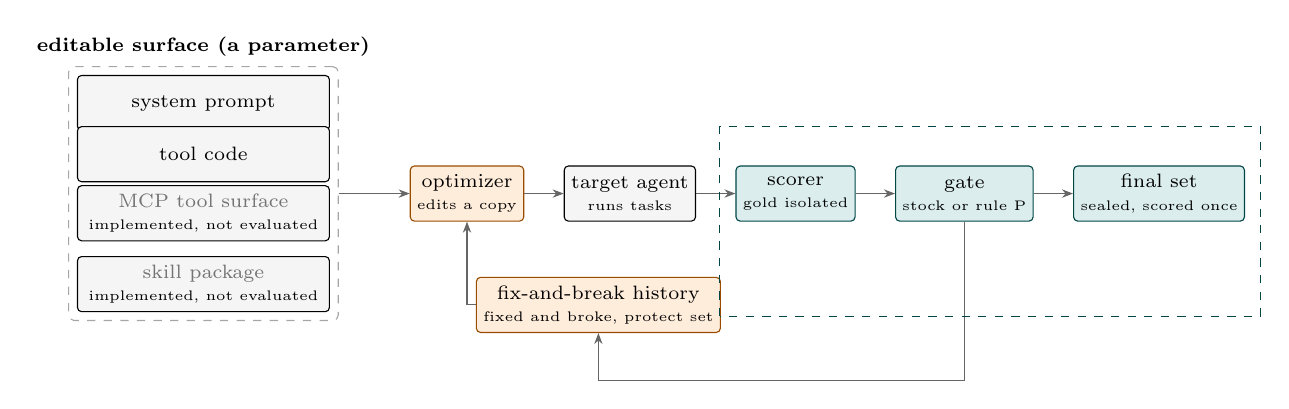
\begin{tikzpicture}[
    font=\scriptsize,
    box/.style={draw,rounded corners=1.5pt,minimum height=7mm,align=center,inner sep=2.5pt,fill=black!4},
    opt/.style={box,fill=orange!14,draw=orange!60!black},
    core/.style={box,fill=teal!14,draw=teal!55!black},
    ar/.style={-{Stealth[length=4pt]},draw=black!60}
  ]
  \node[box,minimum width=32mm] (p) at (0,1.5) {system prompt};
  \node[box,minimum width=32mm] (t) at (0,0.85) {tool code};
  \node[box,minimum width=32mm] (m) at (0,0.1) {\textcolor{black!55}{MCP tool surface}\\{\tiny implemented, not evaluated}};
  \node[box,minimum width=32mm] (k) at (0,-0.8) {\textcolor{black!55}{skill package}\\{\tiny implemented, not evaluated}};
  \node[draw=black!35,dashed,rounded corners=2pt,fit=(p)(t)(m)(k),inner sep=3pt] (surf) {};
  \node[anchor=south,font=\scriptsize\bfseries] at (surf.north) {editable surface (a parameter)};
  \node[opt,right=9mm of surf] (o) {optimizer\\{\tiny edits a copy}};
  \node[box,right=5mm of o] (a) {target agent\\{\tiny runs tasks}};
  \node[core,right=5mm of a] (s) {scorer\\{\tiny gold isolated}};
  \node[core,right=5mm of s] (g) {gate\\{\tiny stock or rule P}};
  \node[core,right=5mm of g] (z) {final set\\{\tiny sealed, scored once}};
  \draw[ar] (surf) -- (o);
  \draw[ar] (o) -- (a); \draw[ar] (a) -- (s); \draw[ar] (s) -- (g); \draw[ar] (g) -- (z);
  \node[opt,below=7mm of a,xshift=-4mm] (h) {fix-and-break history\\{\tiny fixed and broke, protect set}};
  \draw[ar] (h) -| (o);
  \draw[ar] (g.south) |- ([yshift=-6mm]h.east |- h.south) -| (h.south);
  \draw[teal!55!black,dashed] ([xshift=-2mm,yshift=-12mm]s.south west) rectangle ([xshift=2mm,yshift=5mm]z.north east);
  \node[font=\tiny,teal!40!black,anchor=north east] at ([xshift=2mm,yshift=5mm]z.north east) {};
\end{tikzpicture}}%
}

\mlsystitlerunning{CapEvolve: Optimizing Any Editable Surface of a Frozen Agent}

\begin{document}
\twocolumn[
\mlsystitle{\capevolve: Optimizing Any Editable Surface of a Frozen Agent\\Under Code-Owned Evaluation}

\begin{mlsysauthorlist}
\mlsysauthor{Anonymous Author}{anon}
\end{mlsysauthorlist}
\mlsysaffiliation{anon}{Anonymous Institution}
\mlsyscorrespondingauthor{Anonymous Author}{anon@example.com}
\mlsyskeywords{agent optimization, evaluation methodology, skills, prompt optimization, benchmarks}

\vskip 0.3in

\begin{abstract}
Agents run on frozen models, and their behavior is set by files around the model: the prompt, tool code, the tool list exposed over MCP, and skill packages. Optimizers edit these files, but each fixes what it may edit, usually the prompt, and trusts its own scores to decide what to keep. A fixed surface cannot repair a failure that lives elsewhere, and a self-scored accept rule promotes noise.
\capevolve{} makes the editable surface a parameter of one loop, moves every decision an optimizer could game into core code it cannot edit (gold isolation, a two-stage promotion rule, a seal on the final set), and gives the optimizer a causal history of what each earlier edit fixed and broke. It runs as a deterministic hill-climb or as a coding agent driving the same gate.
We evaluate it on SpreadsheetBench and two $\tau^2$-bench domains at a matched rollout checkpoint against nine published optimizers, and ablate the surface, the gate, the orchestration mode and the history.
\pend{[RESULT: headline gain over the seed artifact with interval, standing against the nine competitors, one ablation finding, and what each surface is worth.]}
\needs{Abstract results after the final evaluation; no outcome may be stated before it.}

\end{abstract}
\vspace{0.08in}
\begin{minipage}{\textwidth}
\centering
\loopfigure
\refstepcounter{figure}\label{fig:v2:loop}
\par\vspace{2pt}\begin{small}\emph{Figure \thefigure.} CapEvolve. The editable surface is a parameter of one loop. Orange parts belong to the optimizer; teal parts are core code the optimizer cannot edit. Accepted and rejected candidates feed a fix-and-break history of which tasks each edit fixed and broke. The prompt and tool surfaces are evaluated; the MCP and skill surfaces are implemented, not evaluated.\end{small}
\end{minipage}
\vspace{0.08in}
]

\printAffiliationsAndNotice{}

\section{Introduction}
\label{sec:v2:intro}

Agents run on frozen models, and their behavior is set by the files around the model: the system prompt, tool code, the tool list exposed over MCP, and skill packages \citep{agent_skills_docs}. Optimizers edit these files and report large gains \citep{skillopt,meta-harness}. Published methods span prompt and pipeline optimization \citep{dspy,miprov2-dspy,gepa}, skills \citep{skillopt,evoskill,trace2skill,wikiskill}, context playbooks \citep{ace} and harness search \citep{meta-harness,xu2026harnesslens}. Section~\ref{sec:related} places them by the surface each edits.

Two gaps limit these methods. First, each fixes the object it edits, usually the prompt, so a failure that lives elsewhere is out of reach: a rule the model knows but ignores needs tool code the model cannot skip, and a skipped routine needs a bundled script. Second, acceptance is self-scored. Under trial noise a one-standard-error gate promotes a no-op candidate in \simKoneFalseB{} to \simKoneFalseA{} of ten-candidate searches (Appendix~\ref{app:sim}), and an optimizer that can read gold or the scorer can look better than it is. Our own history shows the cost. An earlier \capevolve{} draft reported a Gemma-4-31B gain of \histGemmaDeltaSaved{} points on SpreadsheetBench; recomputed, scorer compliance explains \histGemmaComplianceShare{}\% of it, and GPT-5.5 shows \histGptComplianceShare{}\% (Appendix~\ref{app:hist}).

\capevolve{} addresses both gaps (Figure~\ref{fig:v2:loop}). The editable surface is a parameter of one loop over four capability types (Section~\ref{sec:v2:surface}). Every decision an optimizer could game moves into core code it cannot edit (Section~\ref{sec:v2:evaluation}). The optimizer receives a causal record of which tasks each earlier edit fixed and broke (Section~\ref{sec:v2:context}), and the loop runs as a deterministic hill-climb or as a coding agent that drives the same gate (Section~\ref{sec:v2:modes}).

We evaluate on SpreadsheetBench (Suite A) and $\tau^2$-bench retail (B) and airline (C), plus a retail ablation family (D), with Claude Sonnet 5.5 as the optimizer for every matched arm. Section~\ref{sec:v2:setup} gives the protocol: a matched rollout checkpoint, official code for eight of nine competitors, and paired, family-clustered statistics with an equivalence rule. \pend{[RESULT: headline gain with interval; standing against nine competitors; one-sentence ablation findings.]}

Our contributions are:
\begin{enumerate}[leftmargin=*,nosep]
\item The editable surface as a parameter, with per-surface edit policies (Section~\ref{sec:v2:surface}).
\item Code-owned evaluation: gold isolation, a two-stage promotion rule with measured operating characteristics, and a final-set seal (Section~\ref{sec:v2:evaluation}).
\item Two orchestration modes over one gate, and a causal optimizer context (Sections~\ref{sec:v2:modes} and~\ref{sec:v2:context}).
\item An agentic intake with a hard adapter gate (Section~\ref{sec:v2:intake}).
\item A matched, audited comparison with nine competitors and ablations of the surface, gate, mode and history (Section~\ref{sec:v2:results}). \pend{[RESULT: one line per ablation.]}
\end{enumerate}

\section{CapEvolve Treats the Editable Surface as a Parameter}
\label{sec:v2:capevolve}

\subsection{One loop, four surfaces}
\label{sec:v2:surface}

A frozen model runs inside an agent assembled from files: a system prompt, the code and descriptions of its tools, the tool list it receives from an MCP server, and skill packages. We call the set of files under optimization the \emph{capability}. \capevolve{} takes the capability type as a parameter of one loop (Table~\ref{tab:v2:surfaces}). The loop is the same for every type: an optimizer edits a copy of the current best capability, the target agent runs on tasks with the candidate live, a scorer returns a reward in $[0,1]$ plus text feedback, and core code accepts or rejects the candidate. What changes with the type is the menu of edits the optimizer is told it may make and the checks that refuse an invalid candidate. Each type ships as a skill with a ``what you can change here'' menu and explicit edit boundaries, and the optimizer prompt is scoped to the selected capability, so an optimizer editing a prompt does not receive tool-editing advice.

The design bet is that failures live on different surfaces. A rule the model knows but does not follow belongs in tool code the model cannot skip. A knowledge gap belongs in the prompt. A skipped multi-step routine belongs in a bundled script. Fixing one surface only forces prose to compensate for errors that belong in code. Section~\ref{sec:v2:results} tests the bet: it edits the prompt on every suite and tool code on the $\tau^2$ suites, and it draws every claim about what a surface is worth from the Suite D ablation, because the main comparison arms change surfaces together. \needs{Skill-package contrast, only if the Suite D skill cell or the Suite A skill cell runs.} The MCP tool surface and skill packages are implemented and unit-tested but not evaluated here.

\begin{table}[t]
\caption{The four editable surfaces and their edit policies, as shipped in the capability skills. A candidate that violates a policy is refused or fails validation before any rollout is paid for.}
\label{tab:v2:surfaces}
\centering\small
\begin{tabularx}{\columnwidth}{@{}p{0.14\columnwidth}XX@{}}
\toprule
Surface & Files edited & Edit policy \\
\midrule
System prompt & Prompt and policy text & Rewrite for clarity, add reasons, consolidate, add rules traceable to the task source, add examples. Never drop a needed rule or broaden a permission. \\
Tools & Tool code, docs and return values & Add guards to existing tool bodies, enrich errors, add composite or loop tools, swap through a wrapper. Never bare-remove a primitive. \\
MCP tool & Client-side descriptions and which tools are shown & Descriptions and exposure only. Schema, handler and new-tool edits are refused. \\
Skill package & \texttt{SKILL.md}, references, scripts & Trigger description, bundled scripts for skipped steps, body, references; the result must stay a valid skill. \\
\bottomrule
\end{tabularx}
\end{table}

\subsection{Agentic intake and a hard adapter gate}
\label{sec:v2:intake}

Spend begins only after an adapter exists and is checked. Intake reads a brief or interviews the user, installs the benchmark, and writes the adapter: how to list tasks per split, how to run the target with a candidate live, how to score a rollout, and where the runner leaves its native traces. It also writes a capability-scoped optimizer prompt that holds benchmark facts only. The check command then refuses to proceed until every required adapter method is real and scoring is deterministic on a fixed rollout, so no budget is spent against a stub. The adapter contract forbids gold in score feedback, but the library does not enforce that (Section~\ref{sec:v2:limits}). Fault injection tests the check (Section~\ref{sec:v2:results}). \needs{Intake cost and time per onboarded benchmark, from run records.}

\subsection{Two orchestration modes over the same gate}
\label{sec:v2:modes}

Hill-climb is deterministic. Each iteration copies the current best candidate, builds a prompt from its per-task rewards (failing, flaky, errored and solid tasks, with the passing tasks listed for protection), lets the optimizer edit the copy, evaluates it on the selection split with $n$ trials per task, applies the gate, and snapshots the candidate whether or not it was accepted (Algorithm~\ref{alg:skeleton} in Appendix~\ref{app:skeleton}). Only an accepted candidate becomes the next parent. Agent-optimize hands the same phases to a coding agent. The agent reads a digest of the budget, noise, failure clusters and branch tips, writes a hypothesis, makes one coherent multi-part edit, and calls a small set of verbs: propose, probe, promote, prune and merge. Candidates form a tree in which any node can be a parent, a probe evaluates only the task and trial cells that a content-addressed ledger lacks, and promotion requires full-split coverage before a judge decides. The two modes differ in who chooses the next experiment and when to stop. They share the splits, the budget counters, the gate and the seal, which core code and plugin hooks enforce.

\subsection{What the optimizer receives}
\label{sec:v2:context}

The optimizer works in a directory that the framework assembles each iteration. It holds the selected capability skill, the diagnosis method, the full trajectories of the current best candidate only (not the seed and every rejected attempt), the supporting source files that new tool code must import, and a fixed/broke record of prior work: for each earlier candidate, the task ids it broke and fixed, and the set of currently passing tasks to protect. Four cross-iteration files keep ownership clean. The framework writes a ledger of facts (outcomes and the exact tasks broken and fixed) and a map to prior iterations with their diffs. The optimizer writes a journal of what it tried, what worked and what regressed, and a process note per candidate. Section~\ref{sec:v2:results} tests whether this history matters by removing it on Suite D. \needs{Suite D history-off result.}

\section{Core Code Owns Every Decision an Optimizer Could Game}
\label{sec:v2:evaluation}

An optimizer that can read the answers, the scorer or the final set can look better than it is, and one that scores itself will bank noise. \capevolve{} therefore moves every such decision into core code that the optimizer cannot edit. Splits are seeded, written once and read back by every skill. The final split is scored once: the run directory raises an error on a second access, and finalization scores the returned candidate and the seed on the same final tasks. The seal blocks scoring and editing but cannot stop reads. Plugin hooks, which live in core-owned scripts and not in editable skill text, deny edits to the sealed test and gold files and block a session from finishing until the adapter check and the gate are green.

Gold isolation has two layers. The adapter gives the target agent a gold-free copy of the task data and scores against the pristine copy. The proposer, a coding-agent subprocess with shell access, runs under a separate user id or in a mount namespace, and a negative test must show denial before launch. The library does not sandbox the proposer itself, so this is a deployment requirement, and a hash manifest over the evaluation surface can detect tampering but cannot stop a read. On the $\tau^2$ suites the evaluator replays the agent's tool calls on the pristine $\tau^2$ toolkit, so edits to tool code change how the agent acts but not how the reference state is computed. Section~\ref{sec:v2:setup} states what was isolated for each arm.

The shipped acceptance rule, the stock gate, is a paired test: accept a candidate when the mean per-task improvement over the current best exceeds $k=1$ standard errors of the paired differences, computed on the selection split only. Hill-climb first sets to zero the tasks whose rollouts never touch the edited files (the edit's footprint) and requires the candidate's own valid fraction to reach 0.6; agent-optimize judges with a $z$-test that has a standard-error floor. About half of all no-op edits measure as a small improvement by chance, so a gate at zero banks noise.

Rule P is the conservative alternative and is off by default. It has two stages. A candidate first passes a screen on the full, unmasked difference vector at $k=1$. It is then confirmed by re-evaluating candidate and incumbent on the same selection tasks with $n_{\mathrm{conf}}$ new trials per task and aligned seeds, and is promoted only if the confirmation improvement is large relative to its standard error ($z_{\mathrm{conf}}$) and enough tasks are covered ($\rho$). The confirmation, not the screen, becomes the next baseline, which removes the selection bias from the reference that later candidates must beat. We froze $n_{\mathrm{conf}}=3$, $z_{\mathrm{conf}}=1.282$, no minimum improvement and $\rho=0.95$ from a budget-exact simulation of one search per suite (Appendix~\ref{app:sim}); Algorithm~\ref{alg:P} gives the rule. Confirmation costs $2\,|D_{\mathrm{sel}}|\,n_{\mathrm{conf}}$ rollouts per screened candidate, charged to the budget.

Table~\ref{tab:sim} gives the operating characteristics, simulated at each suite's observed difficulty and gating-split size, for ten candidates per search, and an empirical check below tests them. In simulation, in an all-null search rule P promotes something falsely with probability \simPFalseA{} on Suite A, \simPFalseB{} on B and \simPFalseC{} on C. The one-stage comparator, an unmasked paired gate with no confirmation, does so with \simKoneFalseA{}, \simKoneFalseB{} and \simKoneFalseC{}; it is not the shipped stock gate, whose footprint mask the simulation omits. Rule P pays in power: a candidate with a true 8-point gain is promoted with probability \simPPowerEightA{}, \simPPowerEightB{} and \simPPowerEightC{}, against \simKonePowerEightA{}, \simKonePowerEightB{} and \simKonePowerEightC{}. Under a stress mix of 60\% null, 25\% positive and 15\% negative edits, the expected true gain of the final artifact is only +\simPGainA{}, +\simPGainB{} and +\simPGainC{} for rule P and +\simKoneGainA{}, +\simKoneGainB{} and +\simKoneGainC{} for the one-stage comparator, so neither exceeds half a point per search. An empirical check is stricter than the simulation. On 40 repeated evaluations of the unmodified Suite D seed (gpt-4.1-mini, 49 tasks), drawing null candidates from the pool, the one-stage unmasked rule promotes at least one of ten null candidates in \nullKone{} of searches (interval \nullKoneLo{} to \nullKoneHi{}), and rule P as run in \nullP{} (\nullPLo{} to \nullPHi{}). Rule P lowers false acceptance about \nullRatio{} times relative to the one-stage rule, but its absolute rate is about \nullPSimRatio{} times what the simulation predicted. The check covers unmasked rules and null edits on a different target from Suite B; it does not test the masked stock gate or true effects. Rule P does not control adaptivity over the task set: the selection tasks also feed the proposer, so a candidate can overfit them and pass both stages. Only the final set removes that bias, and only to the degree it was not reused.

Three further checks guard the measurement. A trial that errors because of the candidate scores zero, while an infrastructure error is retried and, if it persists, scores zero at final scoring (Section~\ref{sec:v2:stats}). The gate refuses to judge when too few tasks are valid on both sides of the pair. Null-edit controls and injected scorer and adapter faults test all of this. \needs{E04 null-edit false-accept rates and the E05 and E06 fault-injection outcomes (15 pass, 7 partial, 6 gap, 1 info at last count), with the gaps stated.}

\section{Experimental Setup}
\label{sec:v2:setup}

\subsection{Suites, models and splits}

Table~\ref{tab:v2:suites} lists the four suites. Suite A edits spreadsheets with a code-execution agent: the target is Gemma-4-31B-it, served by one IBM RITS (Research Inference Service) deployment, on the 400-task verified subset of the 912 SpreadsheetBench questions \citep{spreadsheetbench}\footnote{File \texttt{spreadsheetbench\_verified\_400.tar.gz} (sha256 \texttt{10ef893d}\ldots) in \texttt{github.com/RUCKBReasoning/SpreadsheetBench}, \texttt{data/} directory.}. Suites B and C are customer-service dialogue in $\tau^2$-bench retail and airline \citep{tau2-bench,tau_bench}, pinned at commit 8ebb7499, with gpt-oss-120b as target and user simulator. Suite D is a separate ablation family on retail with an Azure-hosted target (gpt-4.1-mini), which matches Suite B in seed accuracy and trial noise, and the standard gpt-4.1 user simulator and judge. It reuses Suite B's splits and is never pooled with Suites A to C. On Suites B and C GPT-5.5 grades natural-language assertions, because the default judge is not served by our gateway. Claude Sonnet 5.5 is the optimizer or reflection model for every matched arm. One metering gateway tags every model call with suite, arm, search seed and role.

\begin{table}[t]
\caption{Suites. Opt is the tasks whose rollouts the optimizer reads and sel the tasks that gate acceptance; final is scored once per artifact and sized as tasks $\times$ trials. Stock \capevolve{} reads and gates on one validation set. Suite A's final set is a stratified sample of 239 ids from the 912-question release, each scored at most twice before (score only). *Sealed against scoring and selection; the task files were filesystem-visible to the optimizer and no access was observed. $^\dagger$Selection split of 25 tasks plus the sealed 40, up to five trials.}
\label{tab:v2:suites}
\centering\small
\begin{tabularx}{\columnwidth}{@{}lXlll@{}}
\toprule
 & Target & Opt / sel & Final & Exposure \\
\midrule
A & Gemma-4-31B-it & 80 / 40 & $70\times 1$ & score-only exposed \\
B & gpt-oss-120b & 49 / 25 & $40\times 3$ & sealed* \\
C & gpt-oss-120b & 20 / 10 & $20\times 3$ & development-exposed \\
D & gpt-4.1-mini & 49 / 25 & $65\times 5^\dagger$ & sealed* \\
\bottomrule
\end{tabularx}
\end{table}

On Suite A the reward is the LibreOffice-recalculated hard score, and the as-saved score is logged for every rollout. Competitors read train traces and select on validation, while stock \capevolve{} reads and gates on the 40 validation tasks, so it sees 40 tasks where competitors see 120. This differs in exposure, in a direction we cannot sign, and we keep it as the native design. Search-time selection scores are not comparable across methods, since GEPA selects its best on the same tasks it reports, so only final sets are compared. Every arm receives the same scorer feedback, which carries gold-derived facts such as fill counts and error direction but no gold values. Proposers are isolated by user id or mount namespace with a negative test before launch, except where Appendix~\ref{app:incidents} records a gap: on Suite B, agent-optimize can read gold actions of its own optimization and selection tasks. The Suite A final set samples the 239 ids of the 912-question release that remain after removing development-exposed families; we fix the sampling rule and seed and hash the sample before any final-set rollout is scored.

\subsection{Arms and the surface each edits}

Table~\ref{tab:v2:arms} lists the arms. We compare \capevolve{} in three configurations (hill-climb with the stock gate, hill-climb with rule P, agent-optimize with rule P) against nine competitors and two controls, an unoptimized seed artifact and a one-shot repair. Eight of the nine competitors run from official repositories at pinned commits (Appendix~\ref{app:config}); WikiSkill has no official code, so we run a community port. VERSE, CoEvoSkills, and HarnessLens on Suite A failed to reproduce (Appendix~\ref{app:incidents}). Five more methods (AHE, MCE, RHO, Memento-Skills, GraphSkillEvo) are one-seed exploratory runs outside the headline tables. The surface asymmetry matters: on Suites B and C the \capevolve{} arms edit prompt and tools, while GEPA, MIPROv2 and ACE edit the prompt only. Suite A (prompt files for every arm) and the prompt-only cells of Suite D separate loop quality from surface width.

\begin{table}[t]
\caption{Arms and the surface each edits on the suites where it runs. P is prompt text and T is tool code. On Suite A every arm edits the same two prompt files. Main arms run three search seeds to the matched checkpoint; cheap arms run three seeds with a native budget below the cap. Pins are in Appendix~\ref{app:config}.}
\label{tab:v2:arms}
\centering\small
\begin{tabularx}{\columnwidth}{@{}lXc@{}}
\toprule
Arm & Edits and notes & Suites \\
\midrule
\capevolve{} hill-climb & P (A), P+T (B, C, D); stock gate or rule P & A B C D \\
\capevolve{} agent-optimize & P (A), P+T (B, C); rule P & A B C \\
GEPA \citep{gepa} & P; Pareto reflective search & A B C D \\
SkillOpt \citep{skillopt} & train feedback, validation selection & A \\
Meta-Harness \citep{meta-harness} & container-isolated proposer & A \\
EvoSkill \citep{evoskill} & official loop & A \\
WikiSkill \citep{wikiskill} & community port & A \\
Trace2Skill \citep{trace2skill} & cheap, about 200 rollouts & A \\
ACE \citep{ace} & cheap, one output field renamed & A \\
MIPROv2 \citep{miprov2-dspy} & cheap & A \\
HarnessLens \citep{xu2026harnesslens} & native $\tau^2$ fit & B \\
Seed; one-shot repair & shared seed measurement; one unconditional step & A B C D \\
\bottomrule
\end{tabularx}
\end{table}

\subsection{Matched checkpoint and acceptance rules}

Each search may count a budget of $N=600$ target rollouts, every evaluation included, and up to 4M non-cache-read optimizer tokens. One Gemma deployment gives about 12 rollouts per hour per search, so slow arms miss 600. We therefore compare at a matched checkpoint $N^\star$: the largest rollout count that every seed of every primary-family arm reaches by the search cutoff (2026-10-13 06:00 UTC), rounded down to a multiple of 50 and floored at 200, computed from rollout counters only. Other arms are compared at the smaller of $N^\star$ and their own count, and the count is printed beside each number. A candidate whose evaluation straddles $N^\star$ is excluded. Each arm is scored on what its own selection rule would have deployed at $N^\star$. The placeholder values are $N^\star=$ \mockBstarA{}, \mockBstarB{} and \mockBstarC{} for Suites A, B and C. \needs{Final $N^\star$ and the list of incomplete seeds, after the search cutoff.} Suite D cells use a fixed budget of 550 rollouts and are rollout-capped, not checkpoint-matched.

The matching is on target rollouts, not on optimizer compute, which differs by arm; we report optimizer tokens and dollars per arm and claim no compute parity. It is also not on acceptance rules: stock \capevolve{} and the competitors keep their native rules, and rule P is a separate, deliberately conservative configuration. We therefore compare each method together with its own rule, and the stock-gate and rule-P hill-climb arms, plus the Suite D gate cells, measure what the rule costs and buys. A stock-gate secondary family and a selection-to-final shrinkage analysis were added after we saw search-time selection results and are labelled post-search-time. For every arm and seed we report candidates screened, candidates promoted under the native rule, and whether the returned artifact equals the seed artifact. A secondary analysis scores each arm's native end-of-run artifact at the cutoff, labelled unmatched, because truncation at $N^\star$ can penalise schedules tied to the full budget (SkillOpt's cosine schedule, EvoSkill's iteration cap).

\subsection{Ablation family and statistics}
\label{sec:v2:stats}

Suite D changes one factor against a reference cell: hill-climb with the stock gate, prompt and tools, full history. The cells are prompt only, tools only, one-shot repair, rule P, the one-stage gate, and GEPA on the prompt. Candidates are locked to their surface by reading files of a locked surface from the pristine seed, and every violation is counted. The family is registered, with seeds, contrasts and margins, before launch. Its primary Holm family has ten contrasts: prompt only, tools only and prompt+tools each against the seed, prompt+tools against each single surface, rule P and the one-stage gate each against the stock gate, prompt+tools against the one-shot repair, and prompt-only against GEPA on the sealed test only. A secondary family has four contrasts (GEPA, rule P, the one-stage gate and the one-shot repair, each against the seed), and the prompt-tools interaction is a descriptive estimate with an interval and no $p$-value. Everything else is exploratory. The final set is the 25 selection tasks plus the 40 sealed test tasks, five trials per task.

The unit of inference is the task. The headline is the paired contrast with the seed artifact, with cluster-robust standard errors and a $t$ interval, and Holm's step-down adjustment inside each family. The primary family on Suite A pairs hill-climb and agent-optimize with the seed artifact and five competitors (12 contrasts); on B it uses the seed, the one-shot control, GEPA and HarnessLens (8), and on C the seed, the one-shot control and GEPA (6). Each row carries two intervals. The artifact-level interval, used for tests, supports statements about the three frozen artifacts; any statement about the method needs the pipeline-level interval ($t$ with two degrees of freedom, adding seed variance), and if it includes zero we restrict the statement to the frozen artifacts. Per-seed values accompany every mean. Every infrastructure error is retried up to three times with new trial seeds, and a cell that still fails scores 0 for every arm and the seed artifact; hangs past three hours get one retry and then count as missing, and a sensitivity analysis treats failed cells as missing. A win needs a Holm-adjusted $p<0.05$ and an interval that excludes zero. Two artifacts are equivalent only if two one-sided tests at $\alpha=0.05$ both reject for a margin of 10 points; otherwise the result is inconclusive and we do not write ``no difference''.

Variance comes from the seed artifact's observed evaluations (Appendix~\ref{app:sim}). The minimum detectable effect for contrasts between the three frozen artifacts, at 80\% power and $\alpha=0.05$ before Holm, is \mdeACondOne{} points on Suite A (70 tasks, one trial), \mdeBCondThree{} on B and \mdeCCondThree{} on C (three trials); claims about the optimizer itself need \mdeAPipeOne{}, \mdeBPipeThree{} and \mdeCPipeThree{} points. Suite A's seed-artifact mean moved by 8.8 points across six batches, so all arms are scored interleaved in one window. Claude models are priced at list prices as a proxy, and tokens of RITS- and Azure-served models are reported and never counted as zero (Appendix~\ref{app:cost}).

\section{Results}
\label{sec:v2:results}
% GENERATED by scripts/real_results.py from repo files. Audit values are final; cost values are in progress (\prov).
\newcommand{\realAuditGemmaReported}{33.0}
\newcommand{\realAuditGemmaRecalc}{18.7}
\newcommand{\realAuditGptReported}{49.1}
\newcommand{\realAuditGptRecalc}{9.9}
\newcommand{\realAuditClaims}{40}
\newcommand{\realAuditReproduced}{31}
\newcommand{\realAuditContradicted}{2}
\newcommand{\realAuditNoArtifact}{7}
\newcommand{\realCostCalls}{\prov{122\,085}}
\newcommand{\realCostErrors}{\prov{655}}
\newcommand{\realCostLedgerMtok}{\prov{638}}
\newcommand{\realCostUsdLower}{\prov{84}}
\newcommand{\realCostWasteShare}{\prov{22}}
\newcommand{\realCostRitsShare}{\prov{96}}


Section~\ref{sec:v2:cmp} compares \capevolve{} with nine competitors and two controls at a matched checkpoint. Section~\ref{sec:v2:abl} ablates the surface, the orchestration mode and the gate on Suite D and on the main suites. Section~\ref{sec:v2:types} asks what each surface is worth, and Section~\ref{sec:v2:cost} reports cost, regressions and how often the gate says no. Red numbers with a dagger are placeholders and orange numbers are real but still change.
\needs{One sentence with the headline result, written only after the final evaluation.}

\subsection{Comparison at a matched checkpoint}
\label{sec:v2:cmp}

Every difference is paired with the seed artifact on the same tasks, intervals are family-cluster-robust, and p-values are Holm-adjusted inside their family (Section~\ref{sec:v2:stats}). Arms are compared at the matched checkpoint \ckpt{} (\mockBstarA{}, \mockBstarB{} and \mockBstarC{} target rollouts on Suites A, B and C). Table~\ref{tab:main_a} lists \capevolve{} with the stock gate (the shipped configuration), \capevolve{} with rule P, agent-optimize and the competitors against the seed on Suite A, where every arm edits the same two prompt files, so the comparison isolates the loop. The final set has \mockTA{} tasks scored once each for \mockSeedsA{} search seeds per arm, and the seed is scored twice.
\needs{How many arms beat the seed with Holm-adjusted $p<0.05$, which has the largest paired delta, and whether the CapEvolve configurations are above, level with (TOST) or below the best competitor.}

\begin{table*}[t]
\centering
\scriptsize
\setlength{\tabcolsep}{3.5pt}
\caption{Suite A results, baselines by ascending delta and CapEvolve last, with the exploratory stock-gate arm below. Score is the final-set reward. $\Delta$ is the paired difference in points with a family-cluster-robust 95\% interval, $p_{\mathrm{Holm}}$ is Holm-adjusted within the suite, and USD is optimizer cost at Sonnet list prices. Missing is missing over scheduled cells. Tokens and wall clock are in Table~\ref{tab:cost_tokens}, per-seed values in Table~\ref{tab:perseed}, promotions per search in Table~\ref{tab:promotions}. Suite A has no one-shot control. The stock-gate arm (E12A on Suite A, E12C on Suite C) is exploratory and outside the Holm family. (placeholder)}
\label{tab:main_a}
\begin{tabular}{lcccrrr}
\toprule
Arm & Score (\%) & $\Delta$ vs seed [CI] & $p_{\mathrm{Holm}}$ & USD & Missing \\
\midrule
\multicolumn{6}{l}{\textit{Suite A, SpreadsheetBench verified-400 (Gemma-4-31B-it)}} \\
\midrule
Seed (no search) & \pend{50.0} & ref. & -- & -- & \pend{0/140} \\
Meta-Harness & \pend{51.1} & \pend{+1.1 [$-$5.8, +8.0]} & \pend{1.000} & \pend{28} & \pend{0/210} \\
EvoSkill & \pend{52.2} & \pend{+2.2 [$-$4.6, +9.0]} & \pend{1.000} & \pend{17} & \pend{4/210} \\
GEPA & \pend{53.3} & \pend{+3.3 [$-$2.7, +9.4]} & \pend{1.000} & \pend{7} & \pend{5/210} \\
Trace2Skill & \pend{55.2} & \pend{+5.2 [$-$1.6, +12.0]} & \pend{0.687} & \pend{18} & \pend{0/210} \\
MIPROv2 & \pend{55.5} & \pend{+5.5 [$-$0.6, +11.6]} & \pend{0.496} & \pend{11} & \pend{1/210} \\
ACE & \pend{55.8} & \pend{+5.8 [+0.3, +11.3]} & \pend{0.290} & \pend{16} & \pend{5/210} \\
WikiSkill (community) & \pend{55.9} & \pend{+5.9 [$-$0.7, +12.5]} & \pend{0.496} & \pend{6} & \pend{1/210} \\
SkillOpt & \pend{56.7} & \pend{+6.7 [+0.3, +13.1]} & \pend{0.290} & \pend{10} & \pend{1/210} \\
CapEvolve HC & \pend{53.4} & \pend{+3.4 [$-$3.5, +10.3]} & \pend{1.000} & \pend{27} & \pend{5/210} \\
CapEvolve AO & \pend{53.6} & \pend{+3.6 [$-$3.4, +10.6]} & \pend{1.000} & \pend{36} & \pend{9/210} \\
CapEvolve HC, stock gate \textit{(exploratory)} & \pend{54.4} & \pend{+4.4 [$-$2.1, +10.9]} & -- & \pend{37} & \pend{8/210} \\
\bottomrule
\end{tabular}
\end{table*}


On Suites B and C the \capevolve{} arms edit prompt and tools while GEPA, MIPROv2 and ACE edit the prompt only, so a gap there mixes loop quality with surface width. Suite A and the prompt-only cells of Section~\ref{sec:v2:abl} separate the two. Suite B has \mockTB{} sealed test tasks scored \mockTrialsB{} times each and carries the one-shot control (Table~\ref{tab:main_bc}); Suite B has no stock-gate arm, so the shipped gate is not compared there. Suite C reuses the official airline test set of \mockTC{} tasks, which earlier work optimized against, so it is development-exposed and arms are not ranked on it.
\needs{Largest paired delta and number of arms below $p=0.05$ on each of Suites B and C, and whether the ordering agrees with Suite A.}

\begin{table*}[t]
\centering
\scriptsize
\setlength{\tabcolsep}{3.5pt}
\caption{Suites B and C results. Columns as in Table~\ref{tab:main_a}. (placeholder)}
\label{tab:main_bc}
\begin{tabular}{lcccrrr}
\toprule
Arm & Score (\%) & $\Delta$ vs seed [CI] & $\Delta$ vs one-shot [CI] & $p_{\mathrm{Holm}}$ in family & USD & Missing \\
\midrule
\multicolumn{7}{l}{\textit{Suite B, $\tau^2$ retail, sealed test-40 (gpt-oss-120b)}} \\
\midrule
\multicolumn{7}{l}{\textit{Reference arms}} \\
Seed (no search) & \pend{55.0} & ref. & \pend{$-$2.7} & -- & -- & \pend{2/120} \\
One-shot control & \pend{57.7} & \pend{+2.7 [$-$6.4, +11.7]} & ref. & \pend{1.000} & \pend{2} & \pend{5/360} \\
\multicolumn{7}{l}{\textit{Competitors, secondary family}} \\
GEPA & \pend{57.5} & \pend{+2.5 [$-$6.2, +11.2]} & \pend{$-$0.1 [$-$9.7, +9.6]} & \pend{1.000} & \pend{10} & \pend{6/360} \\
HarnessLens & \pend{61.6} & \pend{+6.6 [$-$0.5, +13.6]} & \pend{+3.9 [$-$3.9, +11.8]} & \pend{0.521} & \pend{15} & \pend{2/360} \\
\multicolumn{7}{l}{\textit{CapEvolve, primary family}} \\
CapEvolve HC & \pend{57.2} & \pend{+2.2 [$-$5.5, +9.8]} & \pend{+1.1 [$-$7.5, +9.6]} & \pend{1.000} & \pend{46} & \pend{9/360} \\
CapEvolve AO & \pend{55.3} & \pend{+0.3 [$-$7.7, +8.3]} & \pend{+0.6 [$-$8.3, +9.6]} & \pend{1.000} & \pend{33} & \pend{0/360} \\
\midrule
\multicolumn{7}{l}{\textit{Suite C, $\tau^2$ airline, official test-20 (development-exposed)}} \\
\midrule
\multicolumn{7}{l}{\textit{Reference arms}} \\
Seed (no search) & \pend{40.0} & ref. & \pend{+3.6} & -- & -- & \pend{2/60} \\
One-shot control & \pend{36.4} & \pend{$-$3.6 [$-$17.9, +10.8]} & ref. & \pend{1.000} & \pend{3} & \pend{2/180} \\
\multicolumn{7}{l}{\textit{Competitors, secondary family}} \\
HarnessLens & \pend{42.0} & \pend{+2.0 [$-$11.5, +15.4]} & \pend{+4.1 [$-$10.4, +18.6]} & \pend{1.000} & \pend{6} & \pend{0/180} \\
GEPA & \pend{44.1} & \pend{+4.1 [$-$6.6, +14.9]} & \pend{+8.9 [$-$2.7, +20.5]} & \pend{1.000} & \pend{13} & \pend{8/180} \\
\multicolumn{7}{l}{\textit{CapEvolve, primary family}} \\
CapEvolve HC & \pend{40.0} & \pend{+0.0 [$-$14.3, +14.3]} & \pend{+9.9 [$-$5.5, +25.3]} & \pend{1.000} & \pend{31} & \pend{3/180} \\
CapEvolve AO & \pend{43.9} & \pend{+3.9 [$-$9.9, +17.7]} & \pend{+9.2 [$-$5.7, +24.0]} & \pend{1.000} & \pend{16} & \pend{0/180} \\
\multicolumn{7}{l}{\textit{Exploratory, outside the Holm family}} \\
CapEvolve HC, stock gate & \pend{44.9} & \pend{+4.9 [$-$8.4, +18.2]} & \pend{+8.6 [$-$5.7, +23.0]} & -- & \pend{36} & \pend{1/180} \\
One-shot best of $k$ & \pend{44.5} & \pend{+4.5 [$-$7.1, +16.0]} & \pend{+8.0 [$-$4.5, +20.5]} & -- & \pend{23} & \pend{9/180} \\
\bottomrule
\end{tabular}
\end{table*}


\begin{figure*}[t]
\centering
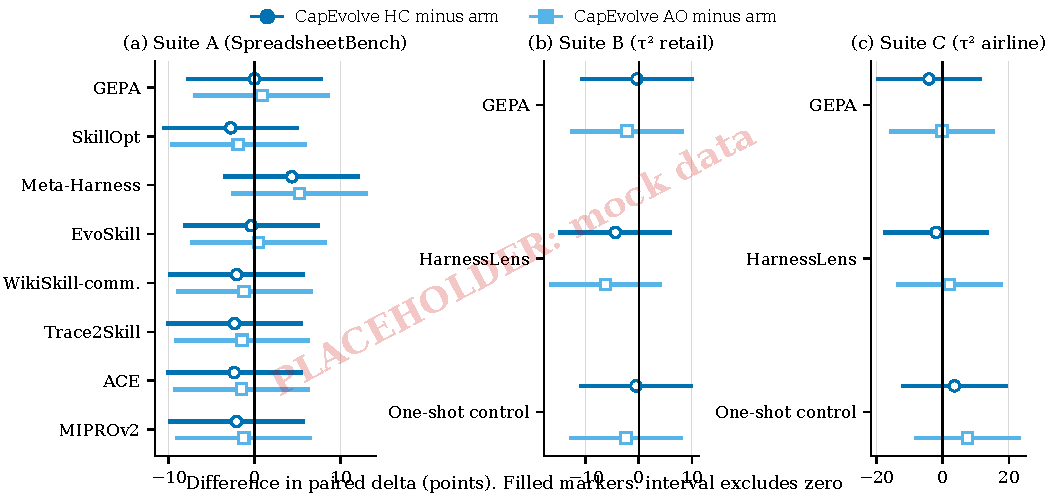
\includegraphics[width=\textwidth]{figures/fig_contrast.pdf}
\caption{Each \capevolve{} configuration against each competitor, as the difference in paired delta in points with 95\% intervals. Filled markers have intervals that exclude zero. These contrasts are the primary family (placeholder).}
\label{fig:contrast}
\end{figure*}

\subsection{Ablations}
\label{sec:v2:abl}

Each ablation changes one factor against the same reference cell and states the claim it tests, with a verdict in the pre-specified vocabulary: supported, equivalent, inconclusive or contradicted.

Surface width. Suite D holds the loop, the stock gate, the budget and the optimizer fixed and edits the prompt only, tools only, or both. The claim is that prompt and tools beats prompt only on tasks whose failures need deterministic enforcement. \needs{Suite D surface grid: paired gains of P, T and P+T over the seed, P+T against each single surface, the interaction term, both intervals, and the verdict. Do not write ``surface width matters'' unless the contrast exceeds the 10-point margin.}

Orchestration. Hill-climb and agent-optimize run on the main suites under rule P. The claim is that they reach equivalent final gain at matched rollouts and differ in cost and failure mode: agent-optimize ended its own search early in several seeds on Suites B and C. \needs{Final-set equivalence verdict (TOST) per suite and the stop reasons of agent-optimize.}

Gate. Rule P is a conservative configuration, and the stock gate is the shipped default. Table~\ref{tab:e12} compares them at the same rollout count on Suites A and C with promotion counts, and Suite D adds a one-stage gate. In simulation at the real task counts rule P falsely promotes in \simPFalseA{}, \simPFalseB{} and \simPFalseC{} of null searches on Suites A, B and C against \simKoneFalseA{}, \simKoneFalseB{} and \simKoneFalseC{} for the one-stage gate, and it promotes a true 8-point gain in \simPPowerEightA{}, \simPPowerEightB{} and \simPPowerEightC{} of searches against \simKonePowerEightA{}, \simKonePowerEightB{} and \simKonePowerEightC{} (Appendix~\ref{app:sim}). Whether the strictness buys held-out reliability or only inertia is answered by the final evaluation. \needs{Final-set gain, promotions per search, inert searches and selection-to-final shrinkage for stock gate, rule P and one-stage gate; null-edit false-accept rates from the empirical null pool.} Search-time promotion counts and shrinkage are post-search-time analyses.

\begin{table}[t]
\centering
\scriptsize
\setlength{\tabcolsep}{3.5pt}
\caption{Stock-gate and rule-P hill-climb at the same rollout count, with per-seed paired deltas to the seed in points and promotion counts (means per search). Descriptive and exploratory: no tests. The best-of-$k$ row draws $k$ independent one-shot proposals per seed on Suite C and keeps the best on the optimization set. It is truncated at $k=6/6/8$ proposals (140/140/180 counted rollouts) for seeds 0/1/2, paused to fund the Suite B stock-gate arm, and is exploratory and descriptive only. (placeholder)}
\label{tab:e12}
\begin{tabular}{lcccccc}
\toprule
Arm & Seed 0 & Seed 1 & Seed 2 & Screened & Promoted & Returned = seed \\
\midrule
\multicolumn{7}{l}{\textit{Suite A}} \\
Rule P & \pend{+0.0} & \pend{+8.1} & \pend{+0.0} & \pend{8.7} & \pend{1.0} & \pend{2 of 3} \\
Stock gate & \pend{+7.4} & \pend{+5.2} & \pend{+6.1} & \pend{8.3} & \pend{6.0} & \pend{0 of 3} \\
\midrule
\multicolumn{7}{l}{\textit{Suite C}} \\
Rule P & \pend{+3.5} & \pend{+2.2} & \pend{+6.7} & \pend{10.3} & \pend{2.3} & \pend{0 of 3} \\
Stock gate & \pend{+4.8} & \pend{+4.6} & \pend{+4.9} & \pend{10.0} & \pend{3.0} & \pend{0 of 3} \\
Best of $k$ & \pend{+3.0} & \pend{+4.7} & \pend{+3.1} & -- & -- & -- \\
\bottomrule
\end{tabular}
\end{table}


Causal history and intake. The history ablation and the descriptions-only and skill-package cells were not approved; Section~\ref{sec:v2:limits} says so. The intake gate was tested by injecting scorer and adapter faults. \needs{Fault-injection summary (pass, partial, gap) with the gaps named.}

\subsection{What each surface is worth}
\label{sec:v2:types}

Marginal value comes from the Suite D grid: each surface's gain over the seed, and the interaction of prompt and tools. \needs{Suite D marginal values with intervals.} The failure types that the seed fails on come from deterministic labels on search-time data, not from the final set: on the $\tau^2$ suites most failed seed tasks are a forgotten required step or a tool call with wrong arguments (Table~\ref{tab:attrib-failure-types}), the kind of failure tool code can enforce, while on Suite A they are output-contract and knowledge failures. Which surface fixed which failure type is an attribution over search-time candidates, and E10 cannot separate surfaces because the main arms edit them together, so we report attribution only as description. \needs{Decision guide: a numbered rule list, each rule traceable to a Suite D or attribution table cell.} The MCP tool surface and the skill package are not evaluated.

\begin{table*}[t]
\centering
\scriptsize
\caption{Failure types of the seed artifact's failed tasks, summed over seeds and trials-pooled tasks. Search-time, failed seed tasks on each run's selection split; deterministic labels from scorer feedback, no model judge, not held-out. Forgotten rule or step: a required write was never called ($\tau^2$). Tool misuse: a write with wrong arguments. Output/contract: no output file (Suite A) or unmet communication assertion ($\tau^2$). Knowledge or rule gap: an output file exists and fails the checks (Suite A).}
\label{tab:attrib-failure-types}
\resizebox{\textwidth}{!}{%
\begin{tabular}{@{}llrrrrrrrr@{}}
\toprule
Suite & Arm & Failed & forgotten rule or step & tool misuse & unexpected side effect & output / contract & knowledge or rule gap & infra (unscorable) & other \\
\midrule
A & CapEvolve AO, rule P & 59 & 0 & 0 & 0 & 26 & 28 & 5 & 0 \\
A & CapEvolve HC, rule P & 54 & 0 & 0 & 0 & 27 & 21 & 6 & 0 \\
A & CapEvolve, stock gate & 57 & 0 & 0 & 0 & 26 & 26 & 5 & 0 \\
B & CapEvolve AO, rule P & 58 & 18 & 24 & 5 & 5 & 0 & 1 & 5 \\
B & CapEvolve HC, rule P & 63 & 23 & 25 & 4 & 3 & 0 & 1 & 7 \\
B & One-shot control & 60 & 17 & 27 & 4 & 5 & 0 & 1 & 6 \\
C & CapEvolve AO, rule P & 29 & 10 & 11 & 5 & 0 & 0 & 0 & 3 \\
C & CapEvolve HC, rule P & 31 & 12 & 13 & 1 & 2 & 0 & 0 & 3 \\
C & CapEvolve, stock gate & 28 & 9 & 12 & 1 & 2 & 0 & 1 & 3 \\
C & One-shot control & 29 & 10 & 11 & 0 & 0 & 0 & 1 & 7 \\
D & D: control (CTL) & 58 & 16 & 23 & 3 & 5 & 0 & 1 & 10 \\
D & D: CapEvolve P & 64 & 22 & 19 & 3 & 6 & 0 & 2 & 12 \\
D & D: CapEvolve P+T & 68 & 28 & 22 & 3 & 5 & 0 & 0 & 10 \\
D & D: CapEvolve T & 62 & 24 & 23 & 5 & 4 & 0 & 0 & 6 \\
D & D: one-stage gate & 67 & 23 & 24 & 2 & 10 & 0 & 2 & 6 \\
D & D: Rule P & 67 & 22 & 25 & 4 & 4 & 0 & 1 & 11 \\
D & D: no history & 61 & 20 & 25 & 2 & 7 & 0 & 0 & 7 \\
\bottomrule
\end{tabular}
}
\end{table*}


\subsection{Cost, regressions and when the gate says no}
\label{sec:v2:cost}

Across the campaign the gateway has metered \costCalls{} calls and \costTokensM{} million non-cache tokens, at least \$\costUsdProxy{} at Sonnet list prices; the bound leaves out RITS and Azure calls, which have no price available to us, and includes smoke tests and restarts that belong to no arm (Appendix~\ref{app:cost}). \needs{Cost per held-out point, regressions against the seed (pass to fail counts), selection-to-final shrinkage and promotions per search for every arm; the cost-quality frontier (Figure~\ref{fig:pareto}).}

\section{Related Work}
\label{sec:related}

Prompt optimizers edit one text artifact. OPRO conditions a model on past (solution, score) pairs \citep{opro}, ProTeGi turns minibatch errors into textual gradients \citep{protegi}, and TextGrad passes textual feedback back through a compound system \citep{textgrad}. MIPROv2 tunes instructions and few-shot demonstrations for each module of a program \citep{miprov2-dspy}. GEPA reflects on rollout traces, keeps a per-task Pareto set of prompts, and merges candidates that share an ancestor \citep{gepa}. We run both from public code. CapEvolve edits a file set (system prompt, tool code, MCP tool descriptions, skill packages) rather than one string, so its search space is wider than any of these methods covers.

Skill and context methods store procedure in text the frozen agent reads. ACE grows a playbook through incremental delta updates to avoid rewriting it wholesale \citep{ace}. EvoSkill diagnoses failures, writes skill folders, and keeps a frontier of programs that score well on a validation set \citep{evoskill}. SkillOpt applies bounded edits to one skill document and accepts an edit only if it strictly improves a held-out selection score \citep{skillopt}. Trace2Skill consolidates many trajectories in parallel into one skill directory \citep{trace2skill}, and WikiSkill co-evolves skills with a persistent wiki \citep{wikiskill}. In the tables of GEPA and SkillOpt, each cell is one score without an interval. We run these methods under one optimizer model and one rollout budget, with three seeds for the main arms, and report intervals. WikiSkill has no official code, so our arm uses a community port.

Harness and agent search edits code. ADAS has a meta agent write new agents in code from an archive of earlier ones \citep{adas}. AFlow searches code-represented workflows with Monte Carlo tree search \citep{aflow}, and AlphaEvolve evolves programs against an automated evaluator \citep{alphaevolve}. The Darwin G\"odel Machine lets a coding agent edit its own code and screens children on 10, then 60, then 200 tasks \citep{dgm}; the Huxley-G\"odel Machine instead guides expansion by an estimate of how well an agent's descendants perform \citep{hgm}. Meta-Harness gives a coding-agent proposer a filesystem holding the code, scores and traces of every earlier candidate \citep{meta-harness}. HarnessLens verifies a candidate only on tasks relevant to its change \citep{xu2026harnesslens}, and DarwinX admits a variant only if it extends the solved set without regressions \citep{darwinx}. CapEvolve's candidate DAG, merge verification and agent-driven controller overlap with these designs, and we do not claim the ideas are new. We ask whether they help once every arm has the same optimizer, budget and final set.

Acceptance rules decide which edit survives. CAPO races candidates and drops weak ones early \citep{capo}, and TRIPLE casts prompt selection as fixed-budget best arm identification \citep{triple}. BudgetAPO sizes evaluation slices from measured task noise \citep{liu2026budgetapo}. SAGE compares candidate and incumbent on the same items with a one-sided paired test \citep{wang2026sage}. PACE uses an anytime-valid e-process, which controls false commits under repeated testing \citep{shawn2026pace}, and a further paper studies when a self-evolving system should stop \citep{yin2026enough}. These rules carry guarantees that our rule P lacks. Rule P (Section~\ref{sec:method:P}) is a paired screen followed by confirmation on fresh trials, tuned by simulation, and its confirmation cost is charged to the search budget.

Evaluation hygiene is an old problem. Reusing a holdout set adaptively makes it a training set \citep{adaptive-data-analysis-holdout-reuse}, and the Ladder limits what a leaderboard reveals for the same reason \citep{ladder}. For agent optimizers, Wang et al.\ report that harness evolution on Terminal-Bench 2.1 does not beat simple test-time scaling under matched feedback and inference budgets, and that earlier work searched on the tasks it reported \citep{rethinkharness}. Meta-Harness states that it searches and scores on the same 89 TerminalBench-2 tasks \citep{meta-harness}. A study of recursive self-evolution finds that removing held-out selection gives a perfect in-sample score and a 33-point drop on test \citep{nguyen2026rsea}. Single-lineage prompt optimization is reported to match or beat GEPA with fewer rollouts \citep{naiveprompt}, and one analysis pass of a coding agent over stored trajectories to beat SkillOpt on all four benchmarks tried \citep{codingagentsopt}. SkillsBench compares matched conditions with and without skills \citep{skillsbench}. We follow this line. Our design adds a scorer audit, gold files hidden from the optimizer, fresh final sets, matched budgets, and one-shot and seed controls.

\section{Limitations and Discussion}
\label{sec:v2:limits}

\begin{itemize}[leftmargin=*,nosep]
\item \emph{We built the system and ran the baselines.} Tuning effort is asymmetric: competitors run through adapters, and every deviation is listed with its expected direction of bias (Appendix~\ref{app:config}); the Suite D contrast with GEPA carries a caveat about a stale target name in GEPA's setting string. On Suites B and C the \capevolve{} arms also edit tools while GEPA does not.
\item \emph{Power.} Three search seeds give two degrees of freedom for statements about the method, and the artifact-level minimum detectable effect is \mdeBCondThree{} points on Suite B and \mdeCCondThree{} on Suite C. We claim at the artifact level and call smaller gaps inconclusive; if no contrast clears Holm, the contribution is the protocol and the audit.
\item \emph{Exposure.} Suite A's final ids were scored at most twice before, score only. The Suite B and D test tasks are scored once and not used by search, but their task files were visible on the runner filesystem; a scan of 68 optimizer transcripts and the run directories found no access, which is absence of evidence. Suite C's test is development-exposed. Pretraining contamination is unchecked.
\item \emph{Gates.} Rule P is conservative and, in the search-time data, held the seed artifact in most searches; the final evaluation decides whether that is reliability or inertia. Stock \capevolve{} gates on a split that also feeds the proposer, so a candidate can overfit it. The stock-gate arm on Suite B (launched 09:56 UTC on 12 October) followed the search-time results, and the secondary family for the arms on A and C was formed after them, so those rows are post-search-time, and agent-optimize on Suites B and C could read its own optimization and selection gold, so its rows carry a dagger and a sensitivity row without it.
\item \emph{Matched checkpoint.} $N^\star$ falls below the nominal budget, so results say little about larger budgets, and we match target rollouts, not optimizer compute.
\item \emph{Ablations.} Suite D uses another target and judge than Suites A to C and establishes mechanism, not rank; surface claims rest on it alone. The MCP and skill surfaces are not evaluated, and intake is tested by fault injection, not a user study.
\item \emph{Scorer and judge.} LibreOffice fails 19 of 400 official gold files as outputs, and GPT-5.5 judges the $\tau^2$ assertions on Suites B and C (Appendix~\ref{app:scorer}).
\end{itemize}


\section{Conclusion}
\label{sec:v2:conclusion}

CapEvolve makes the editable surface a parameter of one loop and keeps every decision an optimizer could game in core code. \needs{Two sentences on the headline comparison and the ablation findings, at the artifact level, after the final evaluation.}


% Marks the last body page for scripts/check_paper.py.
\label{paper:endofbody}

\bibliography{references}
\bibliographystyle{mlsys2025}

\section*{Ethics Statement}
\section{Ethical Considerations}
\label{sec:ethics}

Optimizing against a reward can produce artifacts that score well for the wrong reasons, and editable surfaces that include executable tool code can change what an agent is able to do. We keep the diff, lineage and per-task impact of rejected and accepted candidates, and any optimized artifact considered for deployment needs human review and a rollback path. The audit exposed gold leakage by optimizers; we disclose it rather than hide it, and the isolation tests are in the repository so that other groups can run them. Benchmark tasks drawn from operational systems must be screened for secrets and personal data before release. We rely on provider-hosted and self-hosted models whose usage terms we followed, and the campaign's compute cost is reported in Appendix~\ref{app:cost}.


\clearpage
\onecolumn
\appendix
\section{Configurations}
\label{app:config}

\subsection{Models and decoding}

\begin{table}[h]
\caption{Models and decoding settings as recorded in the model registry and adapters. Prices for Claude models are list-price proxies; other models have no visible price and are reported in tokens only.}
\label{tab:models}
\centering\small
\begin{tabularx}{\textwidth}{@{}lllX@{}}
\toprule
Role & Model & Served by & Settings \\
\midrule
Suite A target & Gemma-4-31B-it & RITS & temperature 0, max tokens 8000, 30 turns, rollout seed 0 \\
Suite B and C target, user simulator & gpt-oss-120b & RITS & temperature 0, max tokens 8000, max steps 100, max errors 10, simulator timeout 7200 s, provider-default reasoning effort \\
Natural-language judge (B, C) & GPT-5.5 & LiteLLM gateway & no temperature sent (the benchmark pins it for this family) \\
Optimizer, all matched arms & Claude Sonnet 5.5 & LiteLLM gateway & Claude Code with 80 turns (Suite A) or 300 turns (Suite B agent-optimize); GEPA reflection 16000 max tokens; SkillOpt optimizer temperature 0.7, 16000 max tokens; MIPROv2 proposer 8000 max tokens; Meta-Harness effort high \\
\bottomrule
\end{tabularx}
\end{table}

\subsection{Shared settings}

Search budget: 600 counted target rollouts, at most 4M non-cache optimizer tokens, seeds 0, 1, 2. Rule P for both \capevolve{} algorithms: $k_{\mathrm{se}}=1$, $n_{\mathrm{conf}}=3$, $z_{\mathrm{conf}}=1.282$, $\delta_{\min}=0$, minimum joint coverage 0.95, footprint gate off, errored trials failed, not dropped. The agent-optimize arm runs the current digest-and-act engine with its stock switches (parallel branching, smart merge, cost gating, failure clustering, pregate and context digest) on, plus active evaluation, and confirms on fresh trials only. The hang rule differs by suite. On Suite A, a rollout hung for 3 hours or more is an infrastructure error with one retry on a new trial seed, counted outside the budget. On Suite B the running jobs use a 2-hour watchdog; GEPA and the controls retry infrastructure errors up to three times inside the budget, while \capevolve{} leaves a missing cell without retry, and HarnessLens uses 3 hours with one retry counted outside the budget. Infrastructure-error counts per arm are reported at the cutoff, and the analysis applies the same missing-cell bounds to every arm.

Suite A uses the SkillOpt split file (80 train, 40 validation, 280 test; file sha256 \texttt{fd40cc4e}\ldots). The seed artifact is \texttt{prompt.md} (sha256 \texttt{aacc289b}\ldots) plus \texttt{task\_template.md} (\texttt{84196741}\ldots). Suite B and C use $\tau^2$-bench at commit \texttt{8ebb7499}. The retail split file hash is \texttt{07d013b7}\ldots; opt, sel and test id-list hash prefixes are \texttt{6d4ef752}, \texttt{694b911b} and \texttt{1e26a51b}. Suite B's 49 optimization tasks are the first 49 of a seeded shuffle (seed 42) of the 74 training ids. Adapter limits differ from benchmark defaults (max steps 100 instead of 200) and are disclosed in every Suite B table.

\subsection{Code pins}

Table~\ref{tab:pins} gives the commits or releases that ran. For each pinned repository, the running copy was compared blob by blob with the tagged tree.

\begin{table}[h]
\caption{Code that ran. ``Blobs'' counts files identical to the pinned tree.}
\label{tab:pins}
\centering\small
\begin{tabularx}{\textwidth}{@{}lXl@{}}
\toprule
Arm & Source and pin & Check \\
\midrule
GEPA & gepa-ai/gepa v0.1.4, commit 8b0ce6c (PyPI 0.1.4); newer head changes resume, cache and engines, not the search loop & 92 of 92 blobs \\
SkillOpt & microsoft/SkillOpt 79124b37; head 343db229 differs in plumbing and docs only & 442 of 442 blobs \\
Meta-Harness & stanford-iris-lab/meta-harness 8123cca, equal to upstream head & clone \\
WikiSkill & community port Stahl-G/wikiskill da6984ca (MIT); no official code exists & clone \\
\capevolve{}, Suite A & campaign branch integration commit ec12d36c9 & merged PRs \\
\capevolve{}, Suite B & campaign head 80aa7ed0c plus tau commit befd2c2b8 & worktree \\
EvoSkill, Trace2Skill, ACE, MIPROv2, HarnessLens & official repositories \needs{pinned commit for each; run records say ``not recorded''} & \\
\bottomrule
\end{tabularx}
\end{table}

\subsection{Per-arm settings from run records}

The tables below are generated from the run records by \texttt{scripts/gen\_config\_tables.py}. They list every setting the records contain; settings the records do not contain are absent.

{\setlength{\tabcolsep}{3pt}
% GENERATED by scripts/gen_config_tables.py. Do not edit by hand.
\subsection*{Suite A}
\small
\begin{longtable}{@{}p{0.17\textwidth}p{0.11\textwidth}p{0.62\textwidth}@{}}
\toprule
Arm & Status & Settings read from the run record (seed 0) \\
\midrule
\endhead
CapEvolve hill-climb & active or finished & algorithm\_\allowbreak\{\}skill=hill-climb; cap=3900000; capabilities=system-prompt; errored\_\allowbreak\{\}trial\_\allowbreak\{\}policy=fail; gate\_\allowbreak\{\}coverage=joint; gate\_\allowbreak\{\}footprint=False; gate\_\allowbreak\{\}k\_\allowbreak\{\}se=1.0; gate\_\allowbreak\{\}min\_\allowbreak\{\}coverage=0.95; gate\_\allowbreak\{\}mode=paired; max\_\allowbreak\{\}iterations=50; max\_\allowbreak\{\}metric\_\allowbreak\{\}calls=600; num\_\allowbreak\{\}trials=1; optimizer\_\allowbreak\{\}max\_\allowbreak\{\}turns=80; optimizer\_\allowbreak\{\}model=aws/claude-sonnet-5-5; optimizer\_\allowbreak\{\}skill=claude-code; optimizer\_\allowbreak\{\}usd\_\allowbreak\{\}per\_\allowbreak\{\}iter=0; pid=1550084; promotion\_\allowbreak\{\}dmin=0.0; promotion\_\allowbreak\{\}k\_\allowbreak\{\}se=1.0; promotion\_\allowbreak\{\}min\_\allowbreak\{\}coverage=0.95; promotion\_\allowbreak\{\}n\_\allowbreak\{\}conf=3; promotion\_\allowbreak\{\}rule=P; promotion\_\allowbreak\{\}z\_\allowbreak\{\}conf=1.282; soft=3500000; stall=0; tag=tag:E10-hill-climb-s0:hill-climb:optimizer; target\_\allowbreak\{\}model=google/gemma-4-31B-it; pin integration\_\allowbreak\{\}sha=ec12d36c9071 \\
CapEvolve agent-optimize & active or finished & algorithm\_\allowbreak\{\}skill=agent-optimize; cap=3900000; capabilities=system-prompt; concurrency=True; confirm\_\allowbreak\{\}fresh\_\allowbreak\{\}only=True; errored\_\allowbreak\{\}trial\_\allowbreak\{\}policy=fail; gate\_\allowbreak\{\}coverage=joint; gate\_\allowbreak\{\}footprint=False; gate\_\allowbreak\{\}k\_\allowbreak\{\}se=1.0; gate\_\allowbreak\{\}min\_\allowbreak\{\}coverage=0.95; gate\_\allowbreak\{\}mode=paired; k-se=1.0`; max-turns=2000; max\_\allowbreak\{\}iterations=50; max\_\allowbreak\{\}metric\_\allowbreak\{\}calls=600; model=aws/claude-sonnet-5-5; n-trials=1`; num\_\allowbreak\{\}trials=1; optimizer\_\allowbreak\{\}max\_\allowbreak\{\}turns=80; optimizer\_\allowbreak\{\}model=aws/claude-sonnet-5-5; optimizer\_\allowbreak\{\}skill=claude-code; optimizer\_\allowbreak\{\}usd\_\allowbreak\{\}per\_\allowbreak\{\}iter=0; orchestration\_\allowbreak\{\}mode=agent; pid=3418219; promotion\_\allowbreak\{\}dmin=0.0; promotion\_\allowbreak\{\}k\_\allowbreak\{\}se=1.0; promotion\_\allowbreak\{\}min\_\allowbreak\{\}coverage=0.95; promotion\_\allowbreak\{\}n\_\allowbreak\{\}conf=3; promotion\_\allowbreak\{\}rule=P; promotion\_\allowbreak\{\}z\_\allowbreak\{\}conf=1.282; propagation=private; soft=3500000; stall=0; tag=tag:E10-agent-optimize-s0:agent-optimize:optimizer; target\_\allowbreak\{\}model=google/gemma-4-31B-it; pin integration\_\allowbreak\{\}sha=ec12d36c9071 \\
GEPA & active or finished & arm=gepa; hard-cap=600; max-metric-calls=555; minibatch=3 \\
SkillOpt & active or finished & accumulation=1; analyst\_\allowbreak\{\}workers=4; arm=skillopt; batch=40; batch\_\allowbreak\{\}size=40; batches\_\allowbreak\{\}per\_\allowbreak\{\}epoch=2; claude\_\allowbreak\{\}trace\_\allowbreak\{\}to\_\allowbreak\{\}optimizer=True; codex\_\allowbreak\{\}trace\_\allowbreak\{\}to\_\allowbreak\{\}optimizer=True; copilot\_\allowbreak\{\}chat\_\allowbreak\{\}optimizer\_\allowbreak\{\}model=; copilot\_\allowbreak\{\}chat\_\allowbreak\{\}target\_\allowbreak\{\}model=; copilot\_\allowbreak\{\}chat\_\allowbreak\{\}timeout=None; copilot\_\allowbreak\{\}exec\_\allowbreak\{\}allow\_\allowbreak\{\}all\_\allowbreak\{\}tools=None; copilot\_\allowbreak\{\}exec\_\allowbreak\{\}home=; copilot\_\allowbreak\{\}exec\_\allowbreak\{\}path=; cursor\_\allowbreak\{\}exec\_\allowbreak\{\}path=; cursor\_\allowbreak\{\}exec\_\allowbreak\{\}sandbox=; data\_\allowbreak\{\}path=; edit\_\allowbreak\{\}budget=4; env=capevolve\_\allowbreak\{\}sb; epochs=3; eval\_\allowbreak\{\}test=False; exec\_\allowbreak\{\}timeout=120; failure\_\allowbreak\{\}only=False; longitudinal\_\allowbreak\{\}pair\_\allowbreak\{\}policy=mixed; lr\_\allowbreak\{\}control\_\allowbreak\{\}mode=fixed; lr\_\allowbreak\{\}scheduler=cosine; max-rollouts=600; max\_\allowbreak\{\}turns=30; merge\_\allowbreak\{\}batch\_\allowbreak\{\}size=8; min\_\allowbreak\{\}edit\_\allowbreak\{\}budget=2; minibatch\_\allowbreak\{\}size=8; minimax\_\allowbreak\{\}api\_\allowbreak\{\}key=; minimax\_\allowbreak\{\}base\_\allowbreak\{\}url=; minimax\_\allowbreak\{\}enable\_\allowbreak\{\}thinking=false; minimax\_\allowbreak\{\}max\_\allowbreak\{\}tokens=8000; minimax\_\allowbreak\{\}model=MiniMax-M3; minimax\_\allowbreak\{\}region=; minimax\_\allowbreak\{\}temperature=0.7; mode=multi; model\_\allowbreak\{\}backend=openai\_\allowbreak\{\}compatible; num\_\allowbreak\{\}epochs=3; optimizer\_\allowbreak\{\}azure\_\allowbreak\{\}openai\_\allowbreak\{\}ad\_\allowbreak\{\}scope=https://cognitiveservices.azure.com/.default; optimizer\_\allowbreak\{\}azure\_\allowbreak\{\}openai\_\allowbreak\{\}api\_\allowbreak\{\}key=; optimizer\_\allowbreak\{\}azure\_\allowbreak\{\}openai\_\allowbreak\{\}api\_\allowbreak\{\}version=2024-12-01-preview; optimizer\_\allowbreak\{\}azure\_\allowbreak\{\}openai\_\allowbreak\{\}auth\_\allowbreak\{\}mode=; optimizer\_\allowbreak\{\}azure\_\allowbreak\{\}openai\_\allowbreak\{\}endpoint=; optimizer\_\allowbreak\{\}azure\_\allowbreak\{\}openai\_\allowbreak\{\}managed\_\allowbreak\{\}identity\_\allowbreak\{\}client\_\allowbreak\{\}id=; optimizer\_\allowbreak\{\}backend=openai\_\allowbreak\{\}compatible; optimizer\_\allowbreak\{\}model=aws/claude-sonnet-5-5; optimizer\_\allowbreak\{\}qwen\_\allowbreak\{\}chat\_\allowbreak\{\}thinking\_\allowbreak\{\}mode=; qwen\_\allowbreak\{\}chat\_\allowbreak\{\}thinking\_\allowbreak\{\}mode=; reasoning\_\allowbreak\{\}effort=medium; rewrite\_\allowbreak\{\}max\_\allowbreak\{\}completion\_\allowbreak\{\}tokens=64000; rewrite\_\allowbreak\{\}reasoning\_\allowbreak\{\}effort=; samples\_\allowbreak\{\}per\_\allowbreak\{\}epoch=80; sel\_\allowbreak\{\}env\_\allowbreak\{\}num=0; skill\_\allowbreak\{\}aware\_\allowbreak\{\}appendix\_\allowbreak\{\}source=both; skill\_\allowbreak\{\}aware\_\allowbreak\{\}consolidate\_\allowbreak\{\}threshold=0; skill\_\allowbreak\{\}update\_\allowbreak\{\}mode=patch; slow\_\allowbreak\{\}update\_\allowbreak\{\}gate\_\allowbreak\{\}with\_\allowbreak\{\}selection=False; slow\_\allowbreak\{\}update\_\allowbreak\{\}samples=20; split\_\allowbreak\{\}mode=split\_\allowbreak\{\}dir; split\_\allowbreak\{\}output\_\allowbreak\{\}dir=; steps\_\allowbreak\{\}per\_\allowbreak\{\}epoch=2; target\_\allowbreak\{\}azure\_\allowbreak\{\}openai\_\allowbreak\{\}ad\_\allowbreak\{\}scope=https://cognitiveservices.azure.com/.default; target\_\allowbreak\{\}azure\_\allowbreak\{\}openai\_\allowbreak\{\}api\_\allowbreak\{\}key=; target\_\allowbreak\{\}azure\_\allowbreak\{\}openai\_\allowbreak\{\}api\_\allowbreak\{\}version=2024-12-01-preview; target\_\allowbreak\{\}azure\_\allowbreak\{\}openai\_\allowbreak\{\}auth\_\allowbreak\{\}mode=; target\_\allowbreak\{\}azure\_\allowbreak\{\}openai\_\allowbreak\{\}endpoint=; target\_\allowbreak\{\}azure\_\allowbreak\{\}openai\_\allowbreak\{\}managed\_\allowbreak\{\}identity\_\allowbreak\{\}client\_\allowbreak\{\}id=; target\_\allowbreak\{\}backend=openai\_\allowbreak\{\}compatible; target\_\allowbreak\{\}model=google/gemma-4-31B-it; target\_\allowbreak\{\}qwen\_\allowbreak\{\}chat\_\allowbreak\{\}thinking\_\allowbreak\{\}mode=; test\_\allowbreak\{\}env\_\allowbreak\{\}num=0; train\_\allowbreak\{\}size=80; use\_\allowbreak\{\}gate=True; use\_\allowbreak\{\}meta\_\allowbreak\{\}skill=True; use\_\allowbreak\{\}skill\_\allowbreak\{\}aware\_\allowbreak\{\}reflection=False; use\_\allowbreak\{\}slow\_\allowbreak\{\}update=True \\
Meta-Harness & active or finished & not recorded \\
EvoSkill & active or finished & not recorded \\
WikiSkill (community) & active or finished & arm=wikiskill; domain=spreadsheet; effort=n/a; engine\_\allowbreak\{\}version=0.2.1; iterations=8; max-rollouts=600; model=google/gemma-4-31B-it; optimizer\_\allowbreak\{\}effort=n/a; optimizer\_\allowbreak\{\}model=aws/claude-sonnet-5-5; timeout=1800; workers=4 \\
Trace2Skill & active or finished & not recorded \\
ACE & active or finished & arm=ace; max-rollouts=600 \\
MIPROv2 & active or finished & arm=mipro; max-rollouts=600 \\
GraphSkillEvo & stopped & not recorded \\
MCE & stopped & not recorded \\
Memento-Skills & stopped & not recorded \\
injtest & active or finished & not recorded \\
\bottomrule
\end{longtable}
\subsection*{Suite B}
\small
\begin{longtable}{@{}p{0.17\textwidth}p{0.11\textwidth}p{0.62\textwidth}@{}}
\toprule
Arm & Status & Settings read from the run record (seed 0) \\
\midrule
\endhead
CapEvolve hill-climb & active or finished & algorithm\_\allowbreak\{\}focus=all; algorithm\_\allowbreak\{\}skill=hill-climb; capabilities=system-prompt,tools; errored\_\allowbreak\{\}trial\_\allowbreak\{\}policy=fail; gate\_\allowbreak\{\}coverage=joint; gate\_\allowbreak\{\}footprint=False; gate\_\allowbreak\{\}k\_\allowbreak\{\}se=1.0; gate\_\allowbreak\{\}min\_\allowbreak\{\}coverage=0.95; gate\_\allowbreak\{\}mode=paired; max\_\allowbreak\{\}iterations=10; max\_\allowbreak\{\}metric\_\allowbreak\{\}calls=550; num\_\allowbreak\{\}trials=1; optimizer\_\allowbreak\{\}max\_\allowbreak\{\}turns=80; optimizer\_\allowbreak\{\}model=aws/claude-sonnet-5-5; optimizer\_\allowbreak\{\}skill=claude-code; optimizer\_\allowbreak\{\}usd\_\allowbreak\{\}per\_\allowbreak\{\}iter=8.0; orchestration\_\allowbreak\{\}mode=deterministic; promotion\_\allowbreak\{\}dmin=0.0; promotion\_\allowbreak\{\}k\_\allowbreak\{\}se=1.0; promotion\_\allowbreak\{\}min\_\allowbreak\{\}coverage=0.95; promotion\_\allowbreak\{\}n\_\allowbreak\{\}conf=3; promotion\_\allowbreak\{\}rule=P; promotion\_\allowbreak\{\}z\_\allowbreak\{\}conf=1.282; split\_\allowbreak\{\}test=0.25; split\_\allowbreak\{\}train=0.5; split\_\allowbreak\{\}val=0.25; stall=0; target\_\allowbreak\{\}model=openai/gpt-oss-120b-a100; pin E10B/WT\_\allowbreak\{\}SHA.txt=befd2c2b8c0e \\
CapEvolve agent-optimize & active or finished & algorithm\_\allowbreak\{\}skill=agent-optimize; capabilities=system-prompt,tools; confirm\_\allowbreak\{\}fresh\_\allowbreak\{\}only=True; errored\_\allowbreak\{\}trial\_\allowbreak\{\}policy=fail; gate\_\allowbreak\{\}coverage=joint; gate\_\allowbreak\{\}footprint=False; gate\_\allowbreak\{\}k\_\allowbreak\{\}se=1.0; gate\_\allowbreak\{\}min\_\allowbreak\{\}coverage=0.95; gate\_\allowbreak\{\}mode=paired; max\_\allowbreak\{\}iterations=10; max\_\allowbreak\{\}metric\_\allowbreak\{\}calls=550; max\_\allowbreak\{\}optimizer\_\allowbreak\{\}usd=40.0; num\_\allowbreak\{\}trials=1; optimizer\_\allowbreak\{\}max\_\allowbreak\{\}turns=300; optimizer\_\allowbreak\{\}model=aws/claude-sonnet-5-5; optimizer\_\allowbreak\{\}skill=claude-code; optimizer\_\allowbreak\{\}usd\_\allowbreak\{\}per\_\allowbreak\{\}iter=8.0; orchestration\_\allowbreak\{\}mode=agent; promotion\_\allowbreak\{\}dmin=0.0; promotion\_\allowbreak\{\}k\_\allowbreak\{\}se=1.0; promotion\_\allowbreak\{\}min\_\allowbreak\{\}coverage=0.95; promotion\_\allowbreak\{\}n\_\allowbreak\{\}conf=3; promotion\_\allowbreak\{\}rule=P; promotion\_\allowbreak\{\}z\_\allowbreak\{\}conf=1.282; split\_\allowbreak\{\}test=0.25; split\_\allowbreak\{\}train=0.5; split\_\allowbreak\{\}val=0.25; stall=0; target\_\allowbreak\{\}model=openai/gpt-oss-120b-a100; pin E10B/WT\_\allowbreak\{\}SHA.txt=befd2c2b8c0e \\
GEPA & active or finished & arm=gepa; exp=E10B; max-metric-calls=600; pin E10B/WT\_\allowbreak\{\}SHA.txt=befd2c2b8c0e \\
HarnessLens & active or finished & not recorded; pin E10B/WT\_\allowbreak\{\}SHA.txt=befd2c2b8c0e \\
Unoptimized seed & active or finished & not recorded; pin E10B/WT\_\allowbreak\{\}SHA.txt=befd2c2b8c0e \\
One-shot repair & active or finished & algorithm\_\allowbreak\{\}focus=all; algorithm\_\allowbreak\{\}skill=hill-climb; capabilities=system-prompt,tools; errored\_\allowbreak\{\}trial\_\allowbreak\{\}policy=fail; gate\_\allowbreak\{\}coverage=joint; gate\_\allowbreak\{\}footprint=False; gate\_\allowbreak\{\}k\_\allowbreak\{\}se=1.0; gate\_\allowbreak\{\}min\_\allowbreak\{\}coverage=0.95; gate\_\allowbreak\{\}mode=paired; max\_\allowbreak\{\}iterations=1; max\_\allowbreak\{\}metric\_\allowbreak\{\}calls=200; num\_\allowbreak\{\}trials=1; optimizer\_\allowbreak\{\}max\_\allowbreak\{\}turns=80; optimizer\_\allowbreak\{\}model=aws/claude-sonnet-5-5; optimizer\_\allowbreak\{\}skill=claude-code; optimizer\_\allowbreak\{\}usd\_\allowbreak\{\}per\_\allowbreak\{\}iter=8.0; orchestration\_\allowbreak\{\}mode=deterministic; split\_\allowbreak\{\}test=0.25; split\_\allowbreak\{\}train=0.5; split\_\allowbreak\{\}val=0.25; stall=0; target\_\allowbreak\{\}model=openai/gpt-oss-120b-a100; pin E10B/WT\_\allowbreak\{\}SHA.txt=befd2c2b8c0e \\
harnesslens\_\allowbreak\{\}ext & active or finished & not recorded; pin E10B/WT\_\allowbreak\{\}SHA.txt=befd2c2b8c0e \\
harnesslens\_\allowbreak\{\}superseded\_\allowbreak\{\}v0 & active or finished & not recorded; pin E10B/WT\_\allowbreak\{\}SHA.txt=befd2c2b8c0e \\
\bottomrule
\end{longtable}
\subsection*{Suite C}
\small
\begin{longtable}{@{}p{0.17\textwidth}p{0.11\textwidth}p{0.62\textwidth}@{}}
\toprule
Arm & Status & Settings read from the run record (seed 0) \\
\midrule
\endhead
CapEvolve hill-climb & active or finished & algorithm\_\allowbreak\{\}focus=all; algorithm\_\allowbreak\{\}skill=hill-climb; capabilities=system-prompt,tools; errored\_\allowbreak\{\}trial\_\allowbreak\{\}policy=fail; gate\_\allowbreak\{\}coverage=joint; gate\_\allowbreak\{\}footprint=False; gate\_\allowbreak\{\}k\_\allowbreak\{\}se=1.0; gate\_\allowbreak\{\}min\_\allowbreak\{\}coverage=0.95; gate\_\allowbreak\{\}mode=paired; max\_\allowbreak\{\}iterations=10; max\_\allowbreak\{\}metric\_\allowbreak\{\}calls=550; num\_\allowbreak\{\}trials=1; optimizer\_\allowbreak\{\}max\_\allowbreak\{\}turns=80; optimizer\_\allowbreak\{\}model=aws/claude-sonnet-5-5; optimizer\_\allowbreak\{\}skill=claude-code; optimizer\_\allowbreak\{\}usd\_\allowbreak\{\}per\_\allowbreak\{\}iter=8.0; orchestration\_\allowbreak\{\}mode=deterministic; promotion\_\allowbreak\{\}dmin=0.0; promotion\_\allowbreak\{\}k\_\allowbreak\{\}se=1.0; promotion\_\allowbreak\{\}min\_\allowbreak\{\}coverage=0.95; promotion\_\allowbreak\{\}n\_\allowbreak\{\}conf=3; promotion\_\allowbreak\{\}rule=P; promotion\_\allowbreak\{\}z\_\allowbreak\{\}conf=1.282; split\_\allowbreak\{\}test=0.25; split\_\allowbreak\{\}train=0.5; split\_\allowbreak\{\}val=0.25; stall=0; target\_\allowbreak\{\}model=openai/gpt-oss-120b-a100; pin tau2\_\allowbreak\{\}pin=8ebb7499622f \\
CapEvolve agent-optimize & active or finished & algorithm\_\allowbreak\{\}skill=agent-optimize; capabilities=system-prompt,tools; confirm\_\allowbreak\{\}fresh\_\allowbreak\{\}only=True; errored\_\allowbreak\{\}trial\_\allowbreak\{\}policy=fail; gate\_\allowbreak\{\}coverage=joint; gate\_\allowbreak\{\}footprint=False; gate\_\allowbreak\{\}k\_\allowbreak\{\}se=1.0; gate\_\allowbreak\{\}min\_\allowbreak\{\}coverage=0.95; gate\_\allowbreak\{\}mode=paired; max\_\allowbreak\{\}iterations=10; max\_\allowbreak\{\}metric\_\allowbreak\{\}calls=550; max\_\allowbreak\{\}optimizer\_\allowbreak\{\}usd=40.0; num\_\allowbreak\{\}trials=1; optimizer\_\allowbreak\{\}max\_\allowbreak\{\}turns=300; optimizer\_\allowbreak\{\}model=aws/claude-sonnet-5-5; optimizer\_\allowbreak\{\}skill=claude-code; optimizer\_\allowbreak\{\}usd\_\allowbreak\{\}per\_\allowbreak\{\}iter=8.0; orchestration\_\allowbreak\{\}mode=agent; promotion\_\allowbreak\{\}dmin=0.0; promotion\_\allowbreak\{\}k\_\allowbreak\{\}se=1.0; promotion\_\allowbreak\{\}min\_\allowbreak\{\}coverage=0.95; promotion\_\allowbreak\{\}n\_\allowbreak\{\}conf=3; promotion\_\allowbreak\{\}rule=P; promotion\_\allowbreak\{\}z\_\allowbreak\{\}conf=1.282; split\_\allowbreak\{\}test=0.25; split\_\allowbreak\{\}train=0.5; split\_\allowbreak\{\}val=0.25; stall=0; target\_\allowbreak\{\}model=openai/gpt-oss-120b-a100; pin tau2\_\allowbreak\{\}pin=8ebb7499622f \\
GEPA & active or finished & arm=gepa; exp=E10C; max-metric-calls=600; pin tau2\_\allowbreak\{\}pin=8ebb7499622f \\
Unoptimized seed & active or finished & not recorded; pin tau2\_\allowbreak\{\}pin=8ebb7499622f \\
One-shot repair & active or finished & algorithm\_\allowbreak\{\}focus=all; algorithm\_\allowbreak\{\}skill=hill-climb; capabilities=system-prompt,tools; errored\_\allowbreak\{\}trial\_\allowbreak\{\}policy=fail; gate\_\allowbreak\{\}coverage=joint; gate\_\allowbreak\{\}footprint=False; gate\_\allowbreak\{\}k\_\allowbreak\{\}se=1.0; gate\_\allowbreak\{\}min\_\allowbreak\{\}coverage=0.95; gate\_\allowbreak\{\}mode=paired; max\_\allowbreak\{\}iterations=1; max\_\allowbreak\{\}metric\_\allowbreak\{\}calls=200; num\_\allowbreak\{\}trials=1; optimizer\_\allowbreak\{\}max\_\allowbreak\{\}turns=80; optimizer\_\allowbreak\{\}model=aws/claude-sonnet-5-5; optimizer\_\allowbreak\{\}skill=claude-code; optimizer\_\allowbreak\{\}usd\_\allowbreak\{\}per\_\allowbreak\{\}iter=8.0; orchestration\_\allowbreak\{\}mode=deterministic; split\_\allowbreak\{\}test=0.25; split\_\allowbreak\{\}train=0.5; split\_\allowbreak\{\}val=0.25; stall=0; target\_\allowbreak\{\}model=openai/gpt-oss-120b-a100; pin tau2\_\allowbreak\{\}pin=8ebb7499622f \\
\bottomrule
\end{longtable}
\noindent Settings differ between seeds for: A/hc/s1, A/hc/s2, A/ao/s1, A/ao/s2, A/evoskill/s1, A/evoskill/s2, B/ao/s2. Values read as ``not recorded'' in the run record are shown as absent, not guessed.

}

\section{Gate Simulation and Statistical Power}
\label{app:sim}

We chose rule P before any main \capevolve{} seed, from a budget-exact simulation on the real promotion and gate code. We then re-ran it at each suite's observed difficulty: the seed artifact's mean reward and trial-level variance on the search split (Suite A: 40 validation tasks, 600 rollouts; Suite B: 49 optimization tasks, 550 rollouts; Suite C: 20 tasks), one screening trial per task, about ten candidates per search and 22{,}400 searches per cell. The pre-declared criterion was to maximise the expected true new-task gain of the final artifact subject to at most 0.15 probability of a false promotion in an all-null search. A search screens 6.7 to 9.4 candidates on average. Table~\ref{tab:sim} gives rule P and the one-stage gate. The false-promotion probability is per search, about one percent per candidate. The gain column is the expected true new-task gain of the final artifact when 60\% of proposed edits are null. The one-stage gate has the larger expected gain and the higher power, and it falsely promotes in about half of all-null searches; rule P gives up power to avoid that. Five confirmation trials at $z_{\mathrm{conf}}=1.645$ would cost $2\cdot 40\cdot 5=400$ of the 600 rollouts per confirmation on Suite A instead of 240, so fewer candidates are screened and the expected gain halves; on Suite B the 490 rollouts exceed the 452 left after the baseline and one screen, so that setting could never promote.

\begin{table}[h]
\caption{Rule P ($n_{\mathrm{conf}}=3$, $z_{\mathrm{conf}}=1.282$) and the one-stage $k=1$ gate, per suite, from simulation at observed difficulty. False prom.\ is the probability of at least one false promotion in an all-null search of about ten candidates. The four power columns give the probability of promoting one candidate with the stated true gain. Gain is the expected true new-task gain of the final artifact.}
\label{tab:sim}
\centering\small
% GENERATED by scripts/derive_numbers.py. Do not edit by hand.
\begin{tabular}{@{}lrrrrr@{}}
\toprule
Rule & False prom. & $+0.04$ & $+0.06$ & $+0.08$ & $+0.10$ \\
\midrule
P, $n_c{=}3$, $z{=}2.0$, $\delta_{\min}{=}0.02$ & 0.014 & 0.03 & 0.08 & 0.15 & 0.26 \\
P, $n_c{=}3$, $z{=}1.645$ & 0.030 & 0.06 & 0.12 & 0.21 & 0.33 \\
P, $n_c{=}3$, $z{=}1.282$ (used) & 0.055 & 0.09 & 0.17 & 0.27 & 0.41 \\
P, $n_c{=}5$, $z{=}1.645$ & 0.019 & 0.08 & 0.16 & 0.29 & 0.42 \\
one-stage, $k{=}1$ & 0.565 & 0.29 & 0.37 & 0.45 & 0.54 \\
one-stage, $k{=}1.645$ & 0.297 & 0.12 & 0.17 & 0.23 & 0.29 \\
\bottomrule
\end{tabular}

\end{table}

Seed-artifact variance replaces the earlier assumptions (mean 0.55, within-task variance 0.149). The observed within-task variance is 0.088, 0.148 and 0.124 on Suites A, B and C, and the standard deviation of the true pass rate across tasks is 0.40, 0.31 and 0.37. With three search seeds, 80\% power, $\alpha=0.05$ and a task-level effect spread of 0.15, the minimum detectable effect for contrasts between the three frozen artifacts is \mdeACondOne{} on Suite A (\mdeATasks{} tasks, one trial), \mdeBCondOne{}, \mdeBCondTwo{} and \mdeBCondThree{} on Suite B (40 tasks, one to three trials) and \mdeCCondOne{}, \mdeCCondTwo{} and \mdeCCondThree{} on Suite C (20 tasks). For claims about the optimizer, which include seed variance and use $t$ with two degrees of freedom, it is \mdeAPipeOne{} on A, \mdeBPipeOne{} to \mdeBPipeThree{} on B and \mdeCPipeOne{} to \mdeCPipeThree{} on C. With Holm correction over the primary family the first-step values rise to \mdeAHolmOne{} on A, \mdeBHolmOne{} on B and \mdeCHolmOne{} on C with one trial. The task-level effect spread, seed-by-task interaction and seed variance cannot be estimated from seed-artifact data and remain assumptions.

The shared standard-error helper adds a within-task term to a variance of task means that already contains it. In simulation (mean reward 0.55, dispersion 1.5, 40 to 280 tasks) its variance is 1.00 times the correct value at one trial per task, 1.33 times at three trials, 1.24 at five and 1.13 at ten for the new-task estimand, and 1.6 to 8.6 times too large for the fixed-task estimand. Its coverage of a new-task target is 0.94 to 0.97. At one trial it equals the between-task term alone.

\section{Scorer Audit}
\label{app:scorer}

The default SpreadsheetBench reward is \texttt{hard\_no\_recalc}: cached values as saved. Correct formula outputs without cached values passed 0 of 30 checks under it and 25 of 30 (LibreOffice 7.1.8.1) to 29 or 30 of 30 (LibreOffice 25.8.7.3) under recalculation. The recalculation path recalculates the candidate output only and uses gold as shipped. With LibreOffice 7.1.8.1 the official gold file used as output fails on 32 of 400 verified tasks, and with 25.8.7.3 on 19. Four verified tasks (130-9, 283-32, 45944, 49300) are unscorable on every path because of malformed answer-position strings, all four in the SkillOpt test split. Scoring was deterministic: 333 records were scored twice with fresh profiles and none differed. The gold workbooks sat in the directory bind-mounted read-write into the agent container; the campaign runs agents on a gold-free copy and scores on the pristine tree.

\section{Historical Results Under Both Scorers}
\label{app:hist}

\begin{table}[h]
\caption{Historical SpreadsheetBench runs (SkillOpt split, 280 test tasks, three optimization runs per row, Opus 5 optimizer) recomputed from run artifacts. Test-280 was development-exposed, so these are fit-quality figures, not held-out results. Paired means; the as-saved delta is the anti-conservative pooled-observation figure of the earlier draft.}
\label{tab:hist}
\centering\small
\begin{tabular}{@{}lrrrr@{}}
\toprule
Target & Baseline as saved & Gain as saved & Baseline recalc. & Gain recalc. \\
\midrule
Gemma-4-31B & \histGemmaBaseSaved{} & +\histGemmaDeltaSaved{} & \histGemmaBaseRecalc{} & +\histGemmaDeltaRecalc{} \\
GPT-5.5 & \histGptBaseSaved{} & +\histGptDeltaSaved{} & \histGptBaseRecalc{} & +\histGptDeltaRecalc{} \\
\bottomrule
\end{tabular}
\end{table}

Disputed and withdrawn claims: the earlier draft quoted 76.5 for Gemma while a blog post quoted 76.8 for the same data (a denominator definition: the post counts the champion on all champion-scored tasks, including four whose seed rollout failed for infrastructure reasons). A GPT-5.5 run with a champion test score of 89.8 against a baseline of 28.9 is excluded: it is a 225-task subset in which 55 champion rollouts failed on a budget error, and the seed scores 38.6 on all 280. Full lists are in \texttt{audit/recomputed\_numbers.csv}.

\section{Infrastructure Incidents}
\label{app:incidents}

Times are UTC on 2026-10-11 unless stated. Each incident lists its effect on the data.
\begin{itemize}[leftmargin=*,nosep]
\item[\emph{EvoSkill priority starvation.}] The gateway's low-priority tag list still contained EvoSkill after its promotion to Tier 1, so under reserved capacity its calls never got a slot between 13:05 and 18:40. Those rollouts show as 1800-second timeouts with zero model calls. They are invalid and kept as \texttt{INVALID} directories; EvoSkill restarted from scratch at 18:25 to 18:55 and is about 5.5 hours behind the other arms.
\item[\emph{Suite B relaunch.}] The first Suite B runs (09:40) used the wrong judge, a pre-merge worktree without rule P, and untagged candidate-tool errors. They were stopped at 12:38, labelled superseded and not used. A second correction restored the agent-optimize seed capability and archived two sessions that ran the archived legacy engine.
\item[\emph{Content-filter rename for ACE.}] Through the gateway, Claude Sonnet 5.5 returns an empty content-filter response when a prompt asks for a chain-of-thought or reasoning field in the output; prose mentions pass. ACE's prompts requested such a field. Its output field was renamed to ``analysis'' with the diff and affected-call count recorded. No other arm was affected.
\item[\emph{HarnessLens retry policy.}] Upstream aborts a whole baseline stage on one worker error. One of six trial rollouts ended with \texttt{opencode\_exit\_1} after a streamed gpt-oss response ended with only reasoning content and no finish reason. HarnessLens is the only arm that streams the target (1 of 98 streamed calls lacked usage). The campaign policy retries a worker error once inside the rollout budget, scores a second error as zero for HarnessLens's internal selection only, and logs every occurrence.
\item[\emph{Gateway call failures.}] At 13:11 we added a transparent retry (three retries, exponential backoff) for connection resets, read timeouts and 502 to 504 responses, and raised the upstream timeout from 900 to 1800 s. Before that, 1 to 2.5\% of Gemma calls failed, and the shared SpreadsheetBench adapter scored such failures as zero for competitor arms while \capevolve{} dropped them. Pre-13:11 zeros remain in competitor histories and are labelled.
\item[\emph{Gold and split-file readability.}] On Suite A the shared proposer user could read split-id files in world-readable checkouts until 10:00; gold and credentials were already denied. A Suite B agent-optimize transcript scan found no read of task or split files, and the arm was moved into a mount-namespace shim at 15:00. Meta-Harness first launched with a gold-readable proposer, stopped before any proposer iteration, and was relaunched container-isolated at 09:38.
\item[\emph{Failed reproductions.}] VERSE needs SWE-rebench or Terminal-Bench docker sessions; CoEvoSkills needs a Harbor per-task loop; HarnessLens on Suite A evolves only OpenCode, Codex and Pi runtimes. Blocker files are in the campaign scratch store.
\end{itemize}

\paragraph{Rollouts scored zero after an infrastructure error.}
Before the 3-hour hang rule, ACE and MIPROv2 first ran with a 40-minute watchdog that scored a timeout as reward zero.
The coordinator rejected it as asymmetric before it produced results: the six 40-minute runs (three seeds per arm) were killed after one counted rollout each, and their event logs hold no watchdog zero.
Zeros that did reach the search come from other adapter paths.
An adapter returns reward 0 with an error string when an LLM call times out at the client or the sandbox returns HTTP 500.
Each such rollout counts against the budget, so the search saw a score and not a missing cell.
We did not check whether the ACE reflector or the MIPROv2 bootstrap showed the error text.

Adapters label these errors differently, so we classify every error row with one rule and keep the adapter label beside it (Table~\ref{tab:zeros}).
Search-time feedback used each method's native handling, and only the reporting is unified.
The rule changes Trace2Skill, WikiSkill, Meta-Harness and GEPA, and leaves SkillOpt as labelled.
Trace2Skill and WikiSkill label all their errors as candidate faults, yet the rule moves 26 and 8 of them to infrastructure: the stored Trace2Skill strings are 8 client timeouts and 18 sandbox 500 errors, and the WikiSkill errors made no target call.
Meta-Harness keeps 27 of its 30 infrastructure labels.
SkillOpt has 27 infrastructure errors and 120 candidate errors, and the 120 are rows where the task template broke its placeholder contract, with no target call.
GEPA's 7 infrastructure labels become candidate errors because they have no string and an unknown call count, and the same happens to 3 Meta-Harness rows and a few Suite B and C rows.
These 18 rows are listed as unverifiable, and raw-log strings would let us reclassify them.
GEPA persists outputs only for its best program, so its counts are incomplete.
The one live timeout zero after the 13:11 gateway fix is MIPROv2 seed 0 at 13:20.
Every other timeout zero before 13:11 enters the sensitivity analysis that treats such rollouts as missing.

\begin{table*}[t]
\centering\scriptsize
\setlength{\tabcolsep}{4pt}
\caption{Error rows per arm and seed under each adapter's own label and under one uniform rule (\texttt{error\_label\_parity.csv}). The rule calls an error infrastructure if it has a transport, timeout or sandbox-HTTP string, or made no target call and kept no string. Every other error is a candidate error, except rows an adapter labelled infrastructure that have no recoverable string and some target calls, which stay unverifiable. Changed counts rows whose class differs from the adapter label. Search used each method's native handling of these errors, and only the reporting is unified. Live runs only.}
\label{tab:zeros}
\begin{tabular}{@{}llrrrrrrrr@{}}
\toprule
Suite & Arm & Seed & Errors & Adapter infra & Adapter candidate & Uniform infra & Uniform candidate & Unverifiable & Changed \\
\midrule
A & ACE & 1 & 1 & 1 & 0 & 1 & 0 & 0 & 0 \\
A & ACE & 2 & 1 & 1 & 0 & 1 & 0 & 0 & 0 \\
A & CapEvolve AO & 0 & 1 & 1 & 0 & 1 & 0 & 0 & 0 \\
A & CapEvolve AO & 1 & 2 & 2 & 0 & 2 & 0 & 0 & 0 \\
A & CapEvolve AO & 2 & 2 & 2 & 0 & 2 & 0 & 0 & 0 \\
A & EvoSkill & 0 & 2 & 2 & 0 & 2 & 0 & 0 & 0 \\
A & EvoSkill & 1 & 2 & 2 & 0 & 2 & 0 & 0 & 0 \\
A & EvoSkill & 2 & 1 & 1 & 0 & 1 & 0 & 0 & 0 \\
A & GEPA & 0 & 1 & 1 & 0 & 1 & 0 & 0 & 0 \\
A & GEPA & 1 & 4 & 4 & 0 & 4 & 0 & 0 & 0 \\
A & GEPA & 2 & 2 & 2 & 0 & 2 & 0 & 0 & 0 \\
A & CapEvolve HC & 0 & 2 & 2 & 0 & 2 & 0 & 0 & 0 \\
A & CapEvolve HC & 1 & 1 & 1 & 0 & 1 & 0 & 0 & 0 \\
A & CapEvolve HC & 2 & 3 & 3 & 0 & 3 & 0 & 0 & 0 \\
A & Meta-Harness & 0 & 6 & 6 & 0 & 6 & 0 & 0 & 0 \\
A & Meta-Harness & 1 & 15 & 15 & 0 & 15 & 0 & 0 & 0 \\
A & Meta-Harness & 2 & 9 & 9 & 0 & 9 & 0 & 0 & 0 \\
A & MIPROv2 & 0 & 3 & 3 & 0 & 3 & 0 & 0 & 0 \\
A & MIPROv2 & 1 & 4 & 4 & 0 & 4 & 0 & 0 & 0 \\
A & SkillOpt & 0 & 85 & 5 & 80 & 5 & 80 & 0 & 0 \\
A & SkillOpt & 1 & 9 & 9 & 0 & 9 & 0 & 0 & 0 \\
A & SkillOpt & 2 & 53 & 13 & 40 & 13 & 40 & 0 & 0 \\
A & Trace2Skill & 0 & 7 & 0 & 7 & 7 & 0 & 0 & 7 \\
A & Trace2Skill & 1 & 6 & 0 & 6 & 5 & 1 & 0 & 5 \\
A & Trace2Skill & 2 & 14 & 0 & 14 & 14 & 0 & 0 & 14 \\
A & WikiSkill & 0 & 3 & 0 & 3 & 3 & 0 & 0 & 3 \\
A & WikiSkill & 1 & 2 & 0 & 2 & 2 & 0 & 0 & 2 \\
A & WikiSkill & 2 & 3 & 0 & 3 & 3 & 0 & 0 & 3 \\
\midrule
B & CapEvolve AO & 0 & 2 & 2 & 0 & 2 & 0 & 0 & 0 \\
B & One-shot control & 0 & 7 & 7 & 0 & 7 & 0 & 0 & 0 \\
B & One-shot control & 1 & 1 & 1 & 0 & 1 & 0 & 0 & 0 \\
B & CapEvolve HC & 0 & 2 & 2 & 0 & 2 & 0 & 0 & 0 \\
B & CapEvolve HC & 1 & 1 & 1 & 0 & 1 & 0 & 0 & 0 \\
B & CapEvolve HC & 2 & 1 & 1 & 0 & 1 & 0 & 0 & 0 \\
\midrule
C & One-shot control & 1 & 1 & 1 & 0 & 1 & 0 & 0 & 0 \\
C & One-shot control & 2 & 1 & 1 & 0 & 1 & 0 & 0 & 0 \\
C & GEPA & 2 & 1 & 1 & 0 & 0 & 0 & 1 & 0 \\
\bottomrule
\end{tabular}
\end{table*}


\section{Cost and Token Totals}
\label{app:cost}

\begin{table}[h]
\caption{Metered usage so far (in progress; final totals follow the search cutoff). Tokens exclude cache reads. Calls include smoke tests, restarts and waste, which the metrics report separately. USD is a Claude-only list-price proxy and a lower bound.}
\label{tab:cost}
\centering\small
\begin{tabular}{@{}lrr@{}}
\toprule
Scope & Calls & Non-cache tokens (M) \\
\midrule
Suite A & \costACalls{} & \costATokensM{} \\
Suite B & \costBCalls{} & \costBTokensM{} \\
Suite C & \costCCalls{} & \costCTokensM{} \\
All, incl.\ smoke and untagged & \costCalls{} & \costTokensM{} \\
\bottomrule
\end{tabular}
\end{table}

Of the total, \costRitsM{}M tokens were served by RITS (uncapped by user decision) and \costNonRitsM{}M by capped gateway models. The proxy-priced total is \$\costUsdProxy{}. \needs{Final per-arm cost table: tokens by role, proxy USD, wall hours and cost per accepted candidate, from analysis/out/metrics after the cutoff.}

\section{Motivating Audit of Historical Results}
\label{app:hist}

This audit is the reason \capevolve{} makes evaluation code-owned (Section~\ref{sec:v2:evaluation}). It covers an earlier version of our own optimizer. Four hazards inflated or obscured its reported results: scorer compliance, split reuse, gold visibility and gate strictness. We recomputed every number below from retained run artifacts (20 SpreadsheetBench runs, none expired) with repository scripts; the audit files list every claim and its status.



\subsection*{The scorer rewards literals over formulas}

The historical SpreadsheetBench scorer loads cached cell values and does not recalculate. A formula written by the agent has no cached value, so it reads as empty and fails. In the verified-400 gold, \histFormulaGoldTasks{} of 400 tasks (\histFormulaGoldPct{}\%) have formula cells in the answer range. Correct formula outputs without cached values passed 0 of 30 checks under the as-saved scorer and 29 to 30 of 30 under LibreOffice recalculation (Appendix~\ref{app:scorer}).

Both metrics were recorded from the same output workbooks, and both gains below are the mean of three paired optimization runs, so only the scorer differs. Gemma-4-31B moved from \histGemmaBaseSaved{} to 76.5 as saved (+\histGemmaDeltaSaved{} points) but from \histGemmaBaseRecalc{} to a recalculated 75.4 to 78.6 (+\histGemmaDeltaRecalc{}). GPT-5.5 gained +\histGptDeltaSaved{} as saved but +\histGptDeltaRecalc{} when its \histGptBaseRecalc{} recalculated baseline is the reference. Formula-to-literal compliance therefore accounts for \histGemmaCompliancePts{} points (\histGemmaComplianceShare{}\%) of the Gemma gain and \histGptCompliancePts{} points (\histGptComplianceShare{}\%) of the GPT-5.5 gain. The recalculating scorer is not free of error either: with LibreOffice 25.8, 19 of 400 official gold files fail as outputs, and 4 tasks are unscorable under any path, so the ceiling on the 280-task test split is 98.6\%.

\subsection*{Development reuse and gold access contaminate the splits}

The historical SpreadsheetBench test split of 280 tasks was scored in development runs, and parts of it served for selection. The airline test-20 and all 87 SkillsBench tasks were exposed the same way (exposure ledger, 17 rows). A one-iteration run from an empty seed artifact reached 85.6 on the 280 tasks where an eight-round agent-optimize run reached 76.4, yet the earlier draft listed the first run only as a 62.9 control. Both are single runs and rank nothing.

Gold answers sat in the directory mounted into the agent container. We found no gold read in 2{,}049 retained agent rollouts, which is an absence of evidence: the retained rollouts cover validation tasks only. On the optimizer side, at least \goldOptimizerRuns{} Claude Code sessions quote gold values or formulas in their notes, and distilled rules appear in champion prompts. One GPT-5.5 session read a prior run's sealed-test evaluation (280 per-task results) and clustered failures by 55 test ids; its champion text is byte-identical to the earlier run's first candidate.

\subsection*{Gate strictness changes which edits are accepted}

The hill-climb gate accepts a candidate whose paired mean gain exceeds one standard error, after setting to zero the tasks whose rollouts never touch the edited files (the edit's footprint). We replayed \replayDecisions{} recorded decisions from \replayRuns{} runs. The recorded rule accepted \replayRecorded{}. An unmasked one-standard-error gate would have accepted \replayUnmasked{}, changed \replayFlipsUnmasked{} decisions, and blocked the champion path in \replayBlockedRuns{} of \replayPathRuns{} runs whose champions later gained on the (exposed) test split. Every recorded-versus-unmasked mismatch in hill-climb runs was a dropped task, not footprint masking, so the footprint concern rests on code and simulation. The replay is descriptive; a two-stage rule cannot be replayed because no artifact re-measures a candidate on new trials. The helper that computes standard errors also double-counts within-task noise, overstating new-task variance by 12 to 33\%; we do not report it (Appendix~\ref{app:sim}).

\subsection*{Scorer audit}
\label{app:scorer}

The default SpreadsheetBench reward is \texttt{hard\_no\_recalc}: cached values as saved. Correct formula outputs without cached values passed 0 of 30 checks under it and 25 of 30 (LibreOffice 7.1.8.1) to 29 or 30 of 30 (LibreOffice 25.8.7.3) under recalculation. The recalculation path recalculates the candidate output only and uses gold as shipped. With LibreOffice 7.1.8.1 the official gold file used as output fails on 32 of 400 verified tasks, and with 25.8.7.3 on 19. Four verified tasks (130-9, 283-32, 45944, 49300) are unscorable on every path because of malformed answer-position strings, all four in the SkillOpt test split. Scoring was deterministic: 333 records were scored twice with fresh profiles and none differed. The gold workbooks sat in the directory bind-mounted read-write into the agent container; the campaign runs agents on a gold-free copy and scores on the pristine tree.

\subsection*{Historical results under both scorers}

\begin{table}[h]
\caption{Historical SpreadsheetBench runs (SkillOpt split, 280 test tasks, three optimization runs per row, Opus 5 optimizer) recomputed from run artifacts. Test-280 was development-exposed, so these are fit-quality figures, not held-out results. Paired means; the as-saved delta is the anti-conservative pooled-observation figure of the earlier draft.}
\label{tab:hist}
\centering\small
\begin{tabular}{@{}lrrrr@{}}
\toprule
Target & Baseline as saved & Gain as saved & Baseline recalc. & Gain recalc. \\
\midrule
Gemma-4-31B & \histGemmaBaseSaved{} & +\histGemmaDeltaSaved{} & \histGemmaBaseRecalc{} & +\histGemmaDeltaRecalc{} \\
GPT-5.5 & \histGptBaseSaved{} & +\histGptDeltaSaved{} & \histGptBaseRecalc{} & +\histGptDeltaRecalc{} \\
\bottomrule
\end{tabular}
\end{table}

Disputed and withdrawn claims: the earlier draft quoted 76.5 for Gemma while a blog post quoted 76.8 for the same data (a denominator definition: the post counts the champion on all champion-scored tasks, including four whose seed rollout failed for infrastructure reasons). A GPT-5.5 run with a champion test score of 89.8 against a baseline of 28.9 is excluded: it is a 225-task subset in which 55 champion rollouts failed on a budget error, and the seed scores 38.6 on all 280. Full lists are in \texttt{audit/recomputed\_numbers.csv}.


\section{Optional Mechanisms (Default Off)}
\label{app:optional}

Both mechanisms below are behind spec switches and change no decision when absent. We do not claim them as new
statistics: merging and subset selection have precedent
\citep{gepa,darwinx,park2026autosaddler,shastri2026bonsai,hgm,xu2026harnesslens}, and our contribution here is
measurement discipline around them.

\emph{Merge verification (\texttt{merge\_\allowbreak verify: true}).}
Given a merge $M$ of branches $A,B$ with common ancestor $P$, the question is whether $A$ and $B$ compose. We evaluate
$P,A,B,M$ on one task block with the \emph{same} fresh trials (one common trial offset, fixed seeds, a runtime check that
the ledger recorded each cell at the offset), and estimate over the block $\mathcal{B}$
\begin{align}
  I &= \mathbb{E}_{x\in\mathcal{B}}\big[\Delta_M(x)-\Delta_A(x)-\Delta_B(x)\big], &
  g &= \mathbb{E}_{x\in\mathcal{B}}\big[\rbar_M(x)-\rbar_{b}(x)\big],
\end{align}
with $\Delta_Y=\rbar_Y-\rbar_P$ and $b$ the parent with the larger block mean. The block is the union of each branch's
observed wins and known losses and $k_s$ seeded random sentinels. The verdict is \emph{pass} iff $|\mathcal{B}|\ge m$,
$g\ge\delta_{\min}$, $z_g\ge z_{\mathrm{pass}}$ and not ($z_I\le -z_{\mathrm{int}}$ and $I\le-\delta_{\min}$);
\emph{loses} if $g<0$ with $z_g\le -z_{\mathrm{lose}}$ or the interaction is significantly negative ($z_I\le -z_{\mathrm{int}}$ and $I\le-\delta_{\min}$) while $g<\delta_{\min}$;
otherwise \emph{inconclusive}, which buys another round of fresh trials up to a cap and then stops, unpromoted. On a loss,
a bounded Zeller delta-debugging search over merged hunks (markdown sections, Python definitions, else files)
localizes the interfering hunks. The parents are always retained, the budget is checked before every arm evaluation and
every debugging test, and the verdict is bound to the content hashes of $P,A,B,M$, which \texttt{promote} re-checks.
% src: AO/merge_verify.py:38-48 (params: n=3, max_rounds=3, n_sentinels=3, dmin=.02, z_pass=1.645, z_lose=1, z_int=1.645,
%   min_block=5, dd_budget=12), 74-89 (select_block), 119-138 (analyse), 141-150 (verdict), 153-173 (run_verification),
%   176-217 (ddmin), 246-272 (hunks); AO/act.py:666-745 (verify_merge: hashes, per-spend check_budget, scratch purge),
%   AO/act.py:518-531 (promote refuses an unverified merge or any hash mismatch); core/cap_evolve/harness.py:371-376 (fixed_seeds)
\emph{Estimand and caveat.} $I$ and $g$ describe the \emph{block}, which is enriched in tasks where $A$ or $B$ won, so
they are not estimates of the population effect of the merge; the population-level decision is the full-split
promotion that follows (rule P when enabled). Fresh trials are what keeps $I$ from being biased negative by selecting
the block on the branches' own wins.

\emph{Screen accounting (\texttt{screen\_\allowbreak accounting: true}).}
A subset screen is treated as a sampling design: its tasks are \emph{affected} (predicted to be reached by the edit),
\emph{sentinels} (regression checks), and a \emph{random} component of $k$ tasks drawn uniformly without replacement
from the remaining pool of size $N_r$, giving inclusion probability $1$ to the first two strata and $k/N_r$ to the third.
The Horvitz--Thompson estimate of the pool-mean delta is
\begin{equation}
  \hat\Delta=\frac1N\Big(\sum_{t\in\text{det}}\Delta_t+\frac{N_r}{k}\sum_{t\in\text{rand}}\Delta_t\Big),
\end{equation}
unbiased over the random draw only if every screened task was measured (otherwise the code clears an \texttt{unbiased}
flag and reports the measured count). The random seed is derived per candidate, and an equal-size uniform subset with an
independent seed is the ablation control. The pool is the validation tasks with a valid parent measurement, and the
record states how many validation tasks fall outside it.
% src: core/cap_evolve/screen_accounting.py:33-38 (derive_seed per candidate), 41-55 (build_screen, pi), 57-66 (build_control),
%   76-111 (ht_estimate, unbiased flag, n_random_measured), 113-130 (record: role scheduling_signal, result false, n_val,
%   pool_excluded); AO/screen.py:183-210 (wiring), 286-289 (record)
\emph{Estimand and caveat.} The estimand is the pool-mean delta of the screened candidate against its parent. A screen
score is a \emph{scheduling signal}: it decides which candidate deserves a full evaluation and is never reported as a
result, and the existing kill-only rule is unchanged (a screen may kill or promote to full evaluation, never accept).
% src: core/cap_evolve/subsample.py:1-40 (kill-only rule); core/cap_evolve/screen_accounting.py:113-130
Selecting among candidates on a fixed draw would still add selection bias to $\hat\Delta$, which the per-candidate seed
mitigates but does not remove.


\section{Measurement Contract Clauses}
\label{app:contract}

\emph{Errored-trial policy.}
A trial that errors is, by default, missing data: it is dropped from the task mean, and a task with no valid trial is
dropped from the paired vector. With \texttt{errored\_\allowbreak trial\_\allowbreak policy: fail}, a trial whose adapter marks the error as
caused by the candidate (\texttt{Rollout.metadata.error\_\allowbreak kind="candidate"}) scores $0$, while every other error stays
missing, so infrastructure faults remain retryable. The framework cannot infer attribution; adapters must set it.
% src: core/cap_evolve/harness.py:287-313 (CANDIDATE_ERROR_KIND, ERRORED_POLICIES, candidate_attributed_error), 496-503
%   (cand_fail reclassification); core/cap_evolve/harness.py:1224-1260 (_paired_deltas drops a task unless both sides have valid trials)
The drop rule is not neutral: a candidate-induced failure treated as missing can raise the apparent delta, which is why
the policy is a switch we report per experiment.

\emph{Joint coverage.}
Coverage is the fraction of \emph{planned} tasks that are valid on \emph{both} sides of the pair. The gate refuses to
judge (returns \emph{indecisive}, which is neither accept nor a rejection of the edit) when coverage is below a floor.
The default coverage is the candidate's own valid fraction; \texttt{gate\_\allowbreak coverage: joint} switches to the paired
definition, and rule P applies its own floor $\rho$ to the confirmation.
% src: core/cap_evolve/harness.py:1189-1220 (planned_val_ids, joint_coverage), 3229-3234 (coverage=jcov when joint, else
%   cand_val.coverage); core/cap_evolve/gate.py:397-406 (coverage < min_coverage -> indecisive); core/cap_evolve/promotion.py:80-92

\emph{Fresh-trial confirmation.}
Rule P's confirmation is the contract's answer to winner's curse within a fixed task set: the evidence that selects a
candidate is not the evidence that promotes it. Seeds are aligned across the two arms so the pair is a true paired
comparison regardless of each artifact's evidence-ledger history.
% src: core/cap_evolve/harness.py:371-376 and 3278-3279; AO/act.py:443-460 (_first_free_trial, _eval_fresh with fixed seeds)


\section{Shared Search Skeleton}
\label{app:skeleton}

\begin{algorithm}[h]
\caption{Shared search skeleton (hill-climb and agent-optimize).}
\label{alg:skeleton}
\begin{algorithmic}[1]
\REQUIRE seed artifact $\artifact_0$, budget $B$, splits $(\Dopt,\Dsel,\Dfin)$, promotion rule $\Pi$
\STATE $\artifact^\star\gets\artifact_0$;\quad $m^\star\gets \mathrm{Eval}(\artifact_0,\Dsel,n_0)$ \COMMENT{baseline measurement}
\WHILE{budget $B$ not exhausted}
  \STATE $\artifact_p\gets \mathrm{SelectParent}()$ \COMMENT{hill-climb: $\artifact^\star$; agent-optimize: any node}
  \STATE $\artifact'\gets \mathrm{Propose}(\artifact_p,\ F_{\Dopt}(\artifact_p))$ \COMMENT{$F$: feedback the proposer may read}
  \IF{protected files of $\artifact'$ were modified}
     \STATE discard $\artifact'$; \textbf{continue} \COMMENT{measurement void, not a zero score}
  \ENDIF
  \STATE $m'\gets \mathrm{Screen}(\artifact',\Dsel)$ \COMMENT{full split or probed cells}
  \IF{$\Pi(\artifact^\star,m^\star,\artifact',m')$ promotes}
     \STATE $\artifact^\star\gets\artifact'$;\quad $m^\star\gets$ the measurement $\Pi$ returns \COMMENT{Algorithm~\ref{alg:P}}
  \ENDIF
\ENDWHILE
\STATE $\mathrm{Finalize}$: score $\artifact^\star$ and $\artifact_0$ once on $\Dfin$ \COMMENT{seal}
\RETURN $\artifact^\star$
\end{algorithmic}
\end{algorithm}

\begin{table}[h]
\centering\small
\caption{Hill-climb and agent-optimize in the shared notation. Entries describe the shipped implementations.}
\label{tab:method:algs}
\footnotesize\begin{tabular}{p{1.9cm}p{4.4cm}p{4.4cm}}
\toprule
 & hill-climb & agent-optimize \\
\midrule
Controller & deterministic loop; one proposer subprocess call per iteration & a conversational driver agent chooses verbs (\texttt{propose}, \texttt{probe}, \texttt{promote}, \texttt{prune}, \texttt{merge}, \texttt{finalize}) \\
Proposer input & instructions rendered from the incumbent's per-task validation rows, and its validation trajectories copied into the working directory & a one-screen digest (budget, noise, failure clusters, branch tips, merge opportunities, pregate warnings) plus validation traces the driver reads itself \\
Feedback visibility & validation only; test is not provided & validation only; ``never view test'' is a prose instruction, not enforced \\
Parent selection & incumbent $\artifact^\star$ & any node of a candidate DAG (\texttt{--parent}); incumbent when parallel branching is off \\
Screen & paired gate on the full validation split for the candidate, optional footprint mask & ledger-driven \emph{probes} of missing (task, trial) cells; optional subset screen (\texttt{screen.py}) \\
Default accept rule & paired one-SE gate over a footprint-masked delta vector, $k_{\mathrm{se}}=1$ in the CLI default & \texttt{reward\_gated} test with a hard-coded SE floor; Beta-posterior rule only when cost gating is off \\
Rule P & opt-in (\texttt{promotion\_\allowbreak rule: P}) & opt-in, same function \\
Stopping & budget caps, consecutive rejects, optional convergence monitor & budget caps; the driver decides when to \texttt{finalize} \\
\bottomrule
\end{tabular}
\end{table}

\begin{algorithm}[h]
\caption{Promotion rule P for candidate $\artifact'$ against incumbent $\artifact^\star$.}
\label{alg:P}
\begin{algorithmic}[1]
\REQUIRE screen measurements $m',m^\star$ on $\Dsel$; $k,\ n_{\mathrm{conf}},\ \delta_{\min},\ z_{\mathrm{conf}},\ \rho$
\STATE $\Delta_t\gets m'_t-m^\star_t$ for $t$ scored on both sides (\emph{unmasked}: no footprint restriction)
\IF{$|\Delta|<2$ \textbf{or} $\bar\Delta\le 0$ \textbf{or} $\bar\Delta\le k\,\SE(\Delta)$} \STATE \textbf{return} reject \ENDIF
\STATE draw one trial offset $o$ (agent-optimize: beyond every trial either artifact has; hill-climb: $o=1000+i\,n_{\mathrm{conf}}$ at iteration $i$); fix seeds as $\mathrm{base}+o+j$
\STATE $m'_{\mathrm{c}}\gets \mathrm{Eval}(\artifact',\Dsel,n_{\mathrm{conf}};o)$;\quad $m^\star_{\mathrm{c}}\gets \mathrm{Eval}(\artifact^\star,\Dsel,n_{\mathrm{conf}};o)$
\STATE $\Delta^{c}_t\gets m'_{\mathrm{c},t}-m^\star_{\mathrm{c},t}$;\quad $\mathrm{cov}\gets |\Delta^{c}|/|\Delta|$
\IF{$\mathrm{cov}<\rho$ \textbf{or} $\bar\Delta^{c}<\delta_{\min}$ \textbf{or} $\bar\Delta^{c}/\SE(\Delta^{c})<z_{\mathrm{conf}}$} \STATE \textbf{return} reject \ENDIF
\RETURN promote, with new baseline $m^\star\gets m'_{\mathrm{c}}$
\end{algorithmic}
\end{algorithm}

\section{Dated Changes to Roster and Parameters}
\label{app:changelog}

All times are UTC on 2026-10-11 unless stated, from the campaign decision log. No final-set score existed at the time of any entry; entries after the searches began (about 14:45) could have seen partial search progress.

\begin{table}[h]
\caption{Changes to the roster, parameters and protocol, in order.}
\label{tab:changelog}
\centering\small
\begin{tabularx}{\textwidth}{@{}l X X@{}}
\toprule
Time & Change & Reason \\
\midrule
09:00 & Suite A roster split into main arms, cheap arms and one-seed exploratory arms & One Gemma deployment saturates; the full roster needed about 70{,}000 rollouts \\
09:55 & EvoSkill promoted to a main arm & A core skill competitor; promoted before any result \\
11:00 & Rule P set to $n_{\mathrm{conf}}=3$, $z_{\mathrm{conf}}=1.282$, $\delta_{\min}=0$ (earlier $10$, $2$, $0.02$) & Earlier values had power 0.15 at a true 8-point gain; chosen by simulation before any main seed \\
11:15 & Comparison moved to a matched checkpoint with a search cutoff of 2026-10-13 06:00 & Fixed 72-hour envelope; checkpoint computed from rollout counters only \\
11:35 & Suite A final set drawn from the 912-question residual pool & Prior test split was development-exposed \\
12:45 & Suite B relaunched with GPT-5.5 judge, rule P and candidate-error tagging & First launch used the wrong judge and a pre-merge worktree \\
13:20 & Suite B roster fixed: hill-climb, agent-optimize, GEPA, HarnessLens as main arms & Saturated gpt-oss deployment; HarnessLens chosen a priori for its native tau fit \\
14:45 & Stock-gate agent-optimize pilot stopped; no live stock-gate arm at that time & Capacity; later reversed by the triage decision to run the stock-gate hill-climb on Suites A and C \\
15:30 & Agent-optimize run on its current engine on both suites & Stock defaults selected an archived legacy loop \\
17:40 & Suite C (tau2 airline) added & User request \\
18:55 & EvoSkill restarted from scratch & Gateway priority misconfiguration invalidated rollouts from 13:05 \\
22:30 & Final sizes pinned: A $70\times 1$, B $40\times 3$, C $20\times 3$ & Capacity and power \\
23:00 & Matched checkpoint computed over primary-family arms only & Slow secondary arms would otherwise bind it \\
\bottomrule
\end{tabularx}
\end{table}

\begin{table}[h]
\caption{Analysis-plan amendments, from the plan's own table. Times are UTC. No held-out or final-set score existed at any of them.}
\label{tab:amendments}
\centering\small
\begin{tabularx}{\textwidth}{@{}l l X X@{}}
\toprule
No. & Date and time & Content & Data seen at the time \\
\midrule
0 & 11 Oct & Base plan & nothing \\
1 & 11 Oct 21:15 & Contrast families, observed-variance MDE, rule-P operating point & seed evaluations on search splits and rollout counters; no candidate outcomes \\
2 & 11 Oct 21:15 to 22:30 & Interleaved window, block sensitivity, empty-output rate, planned sizes & same, plus six seed evaluations on Suite A \\
3 & 11 Oct 22:45 & Equivalence, claim intervals, stock-gate contrasts, promotion counts & same, plus a review round \\
4 & 11 Oct 23:05 & Matched checkpoint over primary-family arms & rollout counters \\
5 & 12 Oct 02:11 & Persistent infrastructure errors score 0 & candidate-level sandbox error rates of one competitor \\
6 & 12 Oct 08:40 & Stock-gate family and shrinkage & search-time selection results; rule P inert (post-search-time) \\
7 & 12 Oct 09:20 & Suite D registration & search-time results of Suites A to C and seed baselines; no Suite D rollout \\
8 & 12 Oct 09:42 (erratum 09:49) & Suite D primary on the test tasks, no-history cell & a review round; no Suite D held-out score \\
9 & 12 Oct 09:55:36 (errata 09:57, 10:00; surface-lock rule 10:00:49) & No single headline, cross-suite rule, inert artifacts, equivalence scope, agent-optimize daggers, stock gate on Suite B & review round 3; search-time results \\
10 & 12 Oct 11:16 (addendum 11:52) & Suite E, airline replication of Suite D; replication rule; search-end rule & Suite A to D search-time results; no Suite D or E held-out score \\
\bottomrule
\end{tabularx}
\end{table}

\section{Ablation, Attribution and Search-Time Tables}
\label{app:v2results}

Tables labelled search-time use each method's own selection split during the search; they are not held-out and are not comparable across methods. Tables without final-set columns are marked pending.

\begin{table}[t]
\centering
\scriptsize
\setlength{\tabcolsep}{3.5pt}
\caption{Stock-gate and rule-P hill-climb at the same rollout count, with per-seed paired deltas to the seed in points and promotion counts (means per search). Descriptive and exploratory: no tests. The best-of-$k$ row draws $k$ independent one-shot proposals per seed on Suite C and keeps the best on the optimization set. It is truncated at $k=6/6/8$ proposals (140/140/180 counted rollouts) for seeds 0/1/2, paused to fund the Suite B stock-gate arm, and is exploratory and descriptive only. (placeholder)}
\label{tab:e12}
\begin{tabular}{lcccccc}
\toprule
Arm & Seed 0 & Seed 1 & Seed 2 & Screened & Promoted & Returned = seed \\
\midrule
\multicolumn{7}{l}{\textit{Suite A}} \\
Rule P & \pend{+0.0} & \pend{+8.1} & \pend{+0.0} & \pend{8.7} & \pend{1.0} & \pend{2 of 3} \\
Stock gate & \pend{+7.4} & \pend{+5.2} & \pend{+6.1} & \pend{8.3} & \pend{6.0} & \pend{0 of 3} \\
\midrule
\multicolumn{7}{l}{\textit{Suite C}} \\
Rule P & \pend{+3.5} & \pend{+2.2} & \pend{+6.7} & \pend{10.3} & \pend{2.3} & \pend{0 of 3} \\
Stock gate & \pend{+4.8} & \pend{+4.6} & \pend{+4.9} & \pend{10.0} & \pend{3.0} & \pend{0 of 3} \\
Best of $k$ & \pend{+3.0} & \pend{+4.7} & \pend{+3.1} & -- & -- & -- \\
\bottomrule
\end{tabular}
\end{table}

\begin{table*}[t]
\centering
\scriptsize
\setlength{\tabcolsep}{3.5pt}
\caption{Suite D ablation cells on the 40 test tasks scored five times each; the 65 held-out tasks (selection and test) are descriptive. All cells are hill-climb with the stock gate except where the gate or the history is the factor. Each cell changes one factor against the PT reference. The Holm family has 11 contrasts. Differences below the pre-registered equivalence margin of 10 points are written inconclusive, not equal. (placeholder)}
\label{tab:ablation}
\begin{tabular}{lcccccrr}
\toprule
Cell & Seeds & $\Delta$ vs seed [CI] & $p_{\mathrm{Holm}}$ vs seed & $\Delta$ vs PT [CI] & $p_{\mathrm{Holm}}$ vs PT & Promoted per search & Returned = seed \\
\midrule
One-shot control & 3 & \pend{+6.3 [$-$5.1, +17.7]} & -- & \pend{$-$0.8 [$-$14.8, +13.2]} & \pend{1.000} & \pend{1.7} & \pend{0 of 3} \\
Prompt only (P) & 3 & \pend{+4.6 [$-$6.0, +15.2]} & \pend{1.000} & \pend{$-$2.5 [$-$16.5, +11.5]} & \pend{1.000} & \pend{5.0} & \pend{0 of 3} \\
Tools only (T) & 3 & \pend{+2.6 [$-$8.2, +13.4]} & \pend{1.000} & \pend{$-$4.5 [$-$18.5, +9.5]} & \pend{1.000} & \pend{4.0} & \pend{0 of 3} \\
Prompt and tools (PT), reference & 3 & \pend{+7.1 [$-$4.6, +18.8]} & \pend{1.000} & ref. & -- & \pend{4.3} & \pend{0 of 3} \\
PT with rule P & 3 & \pend{+7.4 [$-$3.7, +18.5]} & -- & \pend{+0.3 [$-$13.7, +14.3]} & \pend{1.000} & \pend{1.3} & \pend{0 of 3} \\
PT with one-stage gate & 3 & \pend{+2.3 [$-$8.3, +12.9]} & -- & \pend{$-$4.8 [$-$18.8, +9.2]} & \pend{1.000} & \pend{4.3} & \pend{0 of 3} \\
GEPA, prompt only & 3 & \pend{+5.8 [$-$5.5, +17.1]} & -- & \pend{$-$1.3 [$-$15.3, +12.7]} & \pend{1.000} & \pend{2.7} & \pend{0 of 3} \\
PT without fixed/broke history & 3 & \pend{+5.1 [$-$7.1, +17.3]} & -- & \pend{$-$2.0 [$-$16.0, +12.0]} & \pend{1.000} & \pend{4.3} & \pend{0 of 3} \\
\midrule
\multicolumn{8}{l}{Interaction PT $-$ P $-$ T (descriptive): \pend{$-$0.1 [$-$21.7, +21.5]}. P versus T: \pend{+2.0} points, $p_{\mathrm{Holm}}$ \pend{1.000}.} \\
\bottomrule
\end{tabular}
\end{table*}

\begin{table}[t]
\centering
\scriptsize
\setlength{\tabcolsep}{3.5pt}
\caption{Decomposition of Suite D champions that edit both surfaces: paired delta of the whole artifact, of its prompt edits on the seed tools, and of its tool edits on the seed prompt, in points. A gap near zero means the parts add up. (placeholder)}
\label{tab:decomp}
\begin{tabular}{lrrrr}
\toprule
Champion & Whole artifact & Prompt part & Tool part & Whole minus parts \\
\midrule
pt seed 0 & \pend{$-$1.2} & \pend{$-$0.4} & \pend{$-$1.8} & \pend{+1.0} \\
pt seed 1 & \pend{+5.5} & \pend{+3.5} & \pend{+3.8} & \pend{$-$1.8} \\
pt seed 2 & \pend{+10.3} & \pend{+7.3} & \pend{+3.4} & \pend{$-$0.5} \\
rulep seed 0 & \pend{+3.6} & \pend{+2.2} & \pend{+1.9} & \pend{$-$0.4} \\
onestage seed 1 & \pend{+6.5} & \pend{+5.2} & \pend{+3.6} & \pend{$-$2.2} \\
onestage seed 2 & \pend{+5.1} & \pend{+2.1} & \pend{+1.4} & \pend{+1.6} \\
ctl seed 0 & \pend{+5.9} & \pend{+3.6} & \pend{+4.1} & \pend{$-$1.9} \\
pt seed 1 & \pend{+4.3} & \pend{+0.9} & \pend{+2.8} & \pend{+0.6} \\
\bottomrule
\end{tabular}
\end{table}

\begin{table*}[t]
\centering
\scriptsize
\setlength{\tabcolsep}{3.5pt}
\caption{Cost, regressions and selection-to-final shrinkage per arm. USD per point is optimizer cost per seed divided by the final-set gain in points. Pass to fail counts tasks the seed solved and the champion fails, per seed. Shrinkage is selection gain minus final gain, in points, and is zero for a seed that returned the seed artifact. (placeholder)}
\label{tab:rq4}
\begin{tabular}{lrrrrrr}
\toprule
Arm & USD per point & Pass to fail & Protect-set violations & Selection gain & Final gain & Shrinkage \\
\midrule
\multicolumn{7}{l}{\textit{Suite A, SpreadsheetBench verified-400 (Gemma-4-31B-it)}} \\
\midrule
Meta-Harness & \pend{18.7} & \pend{3.1} & \pend{2.5} & \pend{+5.7} & \pend{$-$1.1} & \pend{+6.8} \\
GEPA & \pend{0.8} & \pend{1.4} & \pend{1.6} & \pend{+12.3} & \pend{+3.2} & \pend{+9.1} \\
EvoSkill & \pend{1.5} & \pend{2.7} & \pend{1.7} & \pend{+11.2} & \pend{+3.6} & \pend{+7.6} \\
WikiSkill (community) & \pend{0.4} & \pend{2.4} & \pend{3.2} & \pend{+13.7} & \pend{+5.3} & \pend{+8.4} \\
MIPROv2 & \pend{0.7} & \pend{0.0} & \pend{2.2} & \pend{+15.1} & \pend{+5.3} & \pend{+9.8} \\
Trace2Skill & \pend{1.1} & \pend{3.0} & \pend{1.4} & \pend{+8.8} & \pend{+5.5} & \pend{+3.3} \\
ACE & \pend{1.0} & \pend{4.6} & \pend{1.1} & \pend{+10.2} & \pend{+5.6} & \pend{+4.6} \\
SkillOpt & \pend{0.6} & \pend{0.0} & \pend{2.2} & \pend{+11.3} & \pend{+6.0} & \pend{+5.4} \\
CapEvolve as shipped, stock gate$^{\S}$ & \pend{2.8} & \pend{1.6} & \pend{1.9} & \pend{+6.3} & \pend{+4.4} & \pend{+1.9} \\
CapEvolve HC, rule P & \pend{2.9} & \pend{4.6} & \pend{1.5} & \pend{+7.7} & \pend{+3.2} & \pend{+4.5} \\
CapEvolve AO, rule P & \pend{2.9} & \pend{3.4} & \pend{2.4} & \pend{+5.6} & \pend{+4.1} & \pend{+1.5} \\
\midrule
\multicolumn{7}{l}{\textit{Suite B, $\tau^2$ retail, sealed test-40 (gpt-oss-120b)}} \\
\midrule
HarnessLens & \pend{9.6} & \pend{3.8} & \pend{1.1} & \pend{+2.2} & \pend{$-$1.9} & \pend{+4.1} \\
GEPA & \pend{3.9} & \pend{0.1} & \pend{2.3} & \pend{+7.7} & \pend{+1.3} & \pend{+6.5} \\
CapEvolve HC, rule P & \pend{1.9} & \pend{3.9} & \pend{1.3} & \pend{+8.8} & \pend{+5.7} & \pend{+3.1} \\
CapEvolve AO, rule P & \pend{4.2} & \pend{1.6} & \pend{2.4} & \pend{+10.1} & \pend{+3.5} & \pend{+6.6} \\
\midrule
\multicolumn{7}{l}{\textit{Suite C, $\tau^2$ airline, official test-20 (development-exposed)}} \\
\midrule
GEPA & \pend{1.3} & \pend{2.1} & \pend{1.4} & \pend{+7.6} & \pend{+3.7} & \pend{+3.9} \\
HarnessLens & \pend{0.7} & \pend{3.8} & \pend{2.0} & \pend{+6.8} & \pend{+6.0} & \pend{+0.8} \\
CapEvolve as shipped, stock gate$^{\S}$ & \pend{0.7} & \pend{3.1} & \pend{2.2} & \pend{+7.4} & \pend{+7.4} & \pend{+0.0} \\
CapEvolve HC, rule P & \pend{4.8} & \pend{4.4} & \pend{1.3} & \pend{+7.2} & \pend{+2.6} & \pend{+4.5} \\
CapEvolve AO, rule P & \pend{5.4} & \pend{2.5} & \pend{1.5} & \pend{+5.8} & \pend{+1.6} & \pend{+4.1} \\
\bottomrule
\end{tabular}
\end{table*}

\begin{table*}[t]
\centering
\scriptsize
\caption{Failure types of the seed artifact's failed tasks, summed over seeds and trials-pooled tasks. Search-time, failed seed tasks on each run's selection split; deterministic labels from scorer feedback, no model judge, not held-out. Forgotten rule or step: a required write was never called ($\tau^2$). Tool misuse: a write with wrong arguments. Output/contract: no output file (Suite A) or unmet communication assertion ($\tau^2$). Knowledge or rule gap: an output file exists and fails the checks (Suite A).}
\label{tab:attrib-failure-types}
\resizebox{\textwidth}{!}{%
\begin{tabular}{@{}llrrrrrrrr@{}}
\toprule
Suite & Arm & Failed & forgotten rule or step & tool misuse & unexpected side effect & output / contract & knowledge or rule gap & infra (unscorable) & other \\
\midrule
A & CapEvolve AO, rule P & 59 & 0 & 0 & 0 & 26 & 28 & 5 & 0 \\
A & CapEvolve HC, rule P & 54 & 0 & 0 & 0 & 27 & 21 & 6 & 0 \\
A & CapEvolve, stock gate & 57 & 0 & 0 & 0 & 26 & 26 & 5 & 0 \\
B & CapEvolve AO, rule P & 58 & 18 & 24 & 5 & 5 & 0 & 1 & 5 \\
B & CapEvolve HC, rule P & 63 & 23 & 25 & 4 & 3 & 0 & 1 & 7 \\
B & One-shot control & 60 & 17 & 27 & 4 & 5 & 0 & 1 & 6 \\
C & CapEvolve AO, rule P & 29 & 10 & 11 & 5 & 0 & 0 & 0 & 3 \\
C & CapEvolve HC, rule P & 31 & 12 & 13 & 1 & 2 & 0 & 0 & 3 \\
C & CapEvolve, stock gate & 28 & 9 & 12 & 1 & 2 & 0 & 1 & 3 \\
C & One-shot control & 29 & 10 & 11 & 0 & 0 & 0 & 1 & 7 \\
D & D: control (CTL) & 58 & 16 & 23 & 3 & 5 & 0 & 1 & 10 \\
D & D: CapEvolve P & 64 & 22 & 19 & 3 & 6 & 0 & 2 & 12 \\
D & D: CapEvolve P+T & 68 & 28 & 22 & 3 & 5 & 0 & 0 & 10 \\
D & D: CapEvolve T & 62 & 24 & 23 & 5 & 4 & 0 & 0 & 6 \\
D & D: one-stage gate & 67 & 23 & 24 & 2 & 10 & 0 & 2 & 6 \\
D & D: Rule P & 67 & 22 & 25 & 4 & 4 & 0 & 1 & 11 \\
D & D: no history & 61 & 20 & 25 & 2 & 7 & 0 & 0 & 7 \\
\bottomrule
\end{tabular}
}
\end{table*}

\begin{table*}[t]
\centering
\scriptsize
\caption{Promotions per search and inert searches (the returned artifact equals the seed), per arm. Search-time, each method's own selection split, not held-out. Counts are for the state of each search at the time of the run (still running = searches not yet finished, so inert counts can still change). Promotion definitions differ by method (accepted by the method's own rule) and are not comparable across methods.}
\label{tab:attrib-promotions}
\begin{tabular}{@{}llrrrrrrr@{}}
\toprule
Suite & Arm & Searches & Cands & Promotions & Per search & Inert & Running & Crashed \\
\midrule
A & GEPA & 3 & 40 & 23 & 7.67 & 0 & 3 & 0 \\
A & SkillOpt & 3 & 18 & 11 & 3.67 & 0 & 3 & 0 \\
A & Meta-Harness & 3 & 24 & 10 & 3.33 & 0 & 1 & 0 \\
A & EvoSkill & 3 & 18 & 17 & 5.67 & 0 & 2 & 0 \\
A & WikiSkill-comm. & 3 & 3 & 2 & 0.67 & 1 & 3 & 0 \\
A & Trace2Skill & 3 & 6 & 3 & 1.00 & 0 & 0 & 0 \\
A & ACE & 3 & 0 & 0 & 0.00 & 0 & 3 & 0 \\
A & MIPROv2 & 3 & 20 & 0 & 0.00 & 3 & 3 & 0 \\
A & CapEvolve HC & 3 & 8 & 1 & 0.33 & 2 & 3 & 0 \\
A & CapEvolve AO & 3 & 3 & 0 & 0.00 & 3 & 3 & 0 \\
A-E12 & CapEvolve HC, stock gate & 3 & 19 & 6 & 2.00 & 0 & 3 & 0 \\
B & One-shot control & 3 & 3 & 1 & 0.33 & 2 & 0 & 0 \\
B & GEPA & 3 & 43 & 16 & 5.33 & 0 & 3 & 0 \\
B & HarnessLens & 3 & 0 & 0 & 0.00 & 0 & 1 & 0 \\
B & CapEvolve HC & 3 & 9 & 0 & 0.00 & 3 & 3 & 0 \\
B & CapEvolve AO & 3 & 3 & 0 & 0.00 & 3 & 1 & 0 \\
C & One-shot control & 3 & 3 & 1 & 0.33 & 2 & 0 & 0 \\
C & GEPA & 3 & 27 & 12 & 4.00 & 0 & 3 & 0 \\
C & CapEvolve HC & 3 & 9 & 0 & 0.00 & 3 & 3 & 0 \\
C & CapEvolve AO & 3 & 1 & 0 & 0.00 & 3 & 0 & 0 \\
C-E12 & CapEvolve HC, stock gate & 3 & 16 & 3 & 1.00 & 1 & 3 & 0 \\
C-E12 & Best-of-$k$ & 3 & 15 & 0 & 0.00 & 0 & 3 & 0 \\
\bottomrule
\end{tabular}
\end{table*}

\begin{table*}[t]
\centering
\scriptsize
\caption{Regressions per promotion and net gain for CapEvolve searches. Search-time, own selection split of each run, not held-out. Fixed and broke: tasks moving across the pass line (reward 0.5) relative to the parent. Protect viol.: seed-solid tasks that score below 1 at the candidate. Fresh $\Delta$: promoted candidate minus its baseline on fresh confirmation trials (Rule P only), the least biased within-search gain. Rejected: mean tasks broken by rejected candidates (candidates still pending are excluded).}
\label{tab:attrib-regression}
\begin{tabular}{@{}llrrrrrrrr@{}}
\toprule
Suite & Arm & Cands & Promoted & Fixed/prom. & Broke/prom. & Net/prom. & Broke/rej. & Protect viol./prom. & Fresh $\Delta$/prom. \\
\midrule
A & CapEvolve HC & 5 & 1 & 7.0 & 3.0 & 4.0 & 5.0 & 3.0 & 0.133 \\
A & CapEvolve HC, stock gate & 16 & 6 & 8.3 & 2.5 & 5.8 & 3.4 & 2.2 & -- \\
B & CapEvolve HC & 10 & 0 & -- & -- & -- & 7.2 & -- & -- \\
B & One-shot control & 3 & 1 & 11.0 & 4.0 & 7.0 & 8.0 & 4.0 & -- \\
C & CapEvolve HC & 12 & 0 & -- & -- & -- & 2.0 & -- & -- \\
C & CapEvolve HC, stock gate & 16 & 3 & 4.7 & 1.3 & 3.3 & 3.6 & 1.0 & -- \\
C & One-shot control & 3 & 1 & 5.0 & 1.0 & 4.0 & 2.5 & 1.0 & -- \\
\bottomrule
\end{tabular}
\end{table*}

\begin{table*}[t]
\centering
\scriptsize
\caption{Edit attribution by capability surface for CapEvolve candidates. Search-time, own selection split of each run (A: val-40, B: opt-49, C: opt-20), not held-out. Touching/total candidates, promoted among those touching, mean selection-split change vs parent, mean tasks fixed and broken (pass = reward $\ge$ 0.5), and Spearman correlation between lines changed on the surface and the change. n/a: surface touched by all or none, so no contrast. Selection-split changes are optimistic and noisy.}
\label{tab:attrib-surface}
\resizebox{\textwidth}{!}{%
\begin{tabular}{@{}llllrrrrr@{}}
\toprule
Suite & Arm & Surface & Touch & Promoted & $\Delta$ sel. & Fixed & Broke & $\rho$ \\
\midrule
A & CapEvolve HC, rule P & system\_prompt & 11/11 & 2 & 0.218 & 9.6 & 1.5 & 0.84 \\
A & CapEvolve HC, rule P & task\_template & 11/11 & 2 & 0.218 & 9.6 & 1.5 & 0.40 \\
A & CapEvolve, stock gate & system\_prompt & 36/36 & 7 & 0.017 & 3.6 & 2.9 & -0.53 \\
A & CapEvolve, stock gate & task\_template & 36/36 & 7 & 0.017 & 3.6 & 2.9 & -0.25 \\
B & CapEvolve HC, rule P & system\_prompt & 9/16 & 0 & 0.010 & 7.3 & 6.9 & 0.22 \\
B & CapEvolve HC, rule P & tool\_code & 14/16 & 0 & -0.007 & 6.8 & 7.1 & -0.16 \\
B & One-shot control & system\_prompt & 3/3 & 1 & 0.017 & 7.7 & 6.7 & n/a \\
B & One-shot control & tool\_code & 3/3 & 1 & 0.017 & 7.7 & 6.7 & n/a \\
C & CapEvolve HC, rule P & system\_prompt & 16/16 & 2 & 0.072 & 3.1 & 1.7 & 0.55 \\
C & CapEvolve HC, rule P & tool\_code & 16/16 & 2 & 0.072 & 3.1 & 1.7 & 0.61 \\
C & CapEvolve, stock gate & system\_prompt & 28/29 & 3 & -0.059 & 2.0 & 3.1 & -0.25 \\
C & CapEvolve, stock gate & tool\_code & 29/29 & 3 & -0.062 & 2.0 & 3.2 & -0.29 \\
C & One-shot control & system\_prompt & 3/3 & 1 & 0.088 & 3.7 & 2.0 & n/a \\
C & One-shot control & tool\_code & 3/3 & 1 & 0.088 & 3.7 & 2.0 & n/a \\
\bottomrule
\end{tabular}
}
\end{table*}

\begin{table*}[t]
\centering
\scriptsize
\caption{Surface by failure type: seed-failed tasks fixed by CapEvolve candidates, grouped by the candidate's dominant edited surface (most changed lines). Search-time, fixes counted on each run's selection split over all candidates, promoted ones in parentheses, not held-out. A task counts as fixed when it fails at the parent and passes at the candidate; the count includes noise flips and is not a measure of cause. Types not listed were not fixed.}
\label{tab:attrib-surface-failure}
\resizebox{\textwidth}{!}{%
\begin{tabular}{@{}llrrrrrrrrr@{}}
\toprule
Suite & Dominant surface & communication & infra & missing\_action & no\_output\_file & other & state\_side\_effect & was\_passing\_or\_unlabelled & wrong\_argument & wrong\_result \\
\midrule
A & system\_prompt & 0 (0) & 1 (1) & 0 (0) & 53 (23) & 0 (0) & 0 (0) & 20 (7) & 0 (0) & 44 (26) \\
B & tool\_code & 3 (1) & 0 (0) & 28 (3) & 0 (0) & 11 (1) & 3 (1) & 0 (0) & 37 (5) & 0 (0) \\
B & unavailable & 0 (0) & 0 (0) & 4 (0) & 0 (0) & 2 (0) & 0 (0) & 0 (0) & 3 (0) & 0 (0) \\
C & tool\_code & 4 (0) & 0 (0) & 31 (8) & 0 (0) & 7 (1) & 5 (0) & 5 (2) & 24 (8) & 0 (0) \\
C & unavailable & 2 (0) & 0 (0) & 4 (0) & 0 (0) & 0 (0) & 1 (0) & 0 (0) & 3 (0) & 0 (0) \\
\bottomrule
\end{tabular}}
\end{table*}

\begin{table*}[t]
\centering
\scriptsize
\caption{Selection-to-final shrinkage (selection-split gain minus final-set gain), per arm and seed. PENDING FINAL: the final-set column is empty until the final evaluation (cutoff 2026-10-13 06:00 UTC); the selection gain shown is search-time, on each method's own selection split, not held-out. Seeds that return the seed artifact have shrinkage 0 by construction (amendment 6).}
\label{tab:attrib-shrinkage}
\begin{tabular}{@{}llrrrrl@{}}
\toprule
Suite & Arm & Seed & Sel. gain & Final gain & Shrinkage & Inert \\
\midrule
A & CapEvolve HC, rule P & 0 & 0.171 & -- & -- & no \\
A & CapEvolve HC, rule P & 1 & 0.103 & -- & -- & no \\
A & CapEvolve HC, rule P & 2 & 0.000 & -- & -- & yes \\
A & CapEvolve AO, rule P & 0 & 0.000 & -- & -- & yes \\
A & CapEvolve AO, rule P & 1 & 0.000 & -- & -- & yes \\
A & CapEvolve AO, rule P & 2 & 0.000 & -- & -- & yes \\
A & GEPA & 0 & 0.325 & -- & -- & no \\
A & GEPA & 1 & 0.350 & -- & -- & no \\
A & GEPA & 2 & 0.375 & -- & -- & no \\
A & SkillOpt & 0 & 0.150 & -- & -- & no \\
A & SkillOpt & 1 & 0.300 & -- & -- & no \\
A & SkillOpt & 2 & 0.275 & -- & -- & no \\
A & Meta-Harness & 0 & 0.375 & -- & -- & no \\
A & Meta-Harness & 1 & 0.250 & -- & -- & no \\
A & Meta-Harness & 2 & 0.300 & -- & -- & no \\
A & EvoSkill & 0 & 0.250 & -- & -- & no \\
A & EvoSkill & 1 & 0.325 & -- & -- & no \\
A & EvoSkill & 2 & 0.300 & -- & -- & no \\
A & WikiSkill-comm. & 0 & 0.225 & -- & -- & no \\
A & WikiSkill-comm. & 1 & 0.300 & -- & -- & no \\
A & WikiSkill-comm. & 2 & 0.200 & -- & -- & no \\
A & Trace2Skill & 0 & 0.200 & -- & -- & no \\
A & Trace2Skill & 1 & 0.275 & -- & -- & no \\
A & Trace2Skill & 2 & 0.225 & -- & -- & no \\
A & ACE & 0 & 0.000 & -- & -- & yes \\
A & ACE & 1 & 0.000 & -- & -- & yes \\
A & ACE & 2 & -- & -- & -- & -- \\
A & MIPROv2 & 0 & 0.200 & -- & -- & no \\
A & MIPROv2 & 1 & 0.300 & -- & -- & no \\
A & MIPROv2 & 2 & 0.050 & -- & -- & no \\
B & CapEvolve HC, rule P & 0 & 0.000 & -- & -- & yes \\
B & CapEvolve HC, rule P & 1 & 0.000 & -- & -- & yes \\
B & CapEvolve HC, rule P & 2 & 0.000 & -- & -- & yes \\
B & CapEvolve AO, rule P & 0 & 0.000 & -- & -- & yes \\
B & CapEvolve AO, rule P & 1 & 0.000 & -- & -- & yes \\
B & CapEvolve AO, rule P & 2 & 0.000 & -- & -- & yes \\
B & GEPA & 0 & 0.160 & -- & -- & no \\
B & GEPA & 1 & 0.360 & -- & -- & no \\
B & GEPA & 2 & 0.120 & -- & -- & no \\
B & HarnessLens & 0 & -- & -- & -- & -- \\
B & HarnessLens & 1 & -- & -- & -- & -- \\
B & HarnessLens & 2 & -- & -- & -- & -- \\
B & One-shot control & 0 & 0.000 & -- & -- & yes \\
B & One-shot control & 1 & 0.143 & -- & -- & no \\
B & One-shot control & 2 & 0.000 & -- & -- & yes \\
C & CapEvolve HC, rule P & 0 & 0.150 & -- & -- & no \\
C & CapEvolve HC, rule P & 1 & 0.000 & -- & -- & yes \\
C & CapEvolve HC, rule P & 2 & 0.134 & -- & -- & no \\
C & CapEvolve AO, rule P & 0 & 0.000 & -- & -- & yes \\
C & CapEvolve AO, rule P & 1 & 0.000 & -- & -- & yes \\
C & CapEvolve AO, rule P & 2 & 0.000 & -- & -- & yes \\
C & GEPA & 0 & 0.200 & -- & -- & no \\
C & GEPA & 1 & 0.200 & -- & -- & no \\
C & GEPA & 2 & 0.100 & -- & -- & no \\
C & One-shot control & 0 & 0.237 & -- & -- & no \\
C & One-shot control & 1 & 0.000 & -- & -- & yes \\
C & One-shot control & 2 & 0.000 & -- & -- & yes \\
A-E12 & CapEvolve, stock gate & 0 & 0.286 & -- & -- & no \\
A-E12 & CapEvolve, stock gate & 1 & 0.349 & -- & -- & no \\
A-E12 & CapEvolve, stock gate & 2 & 0.322 & -- & -- & no \\
C-E12 & CapEvolve, stock gate & 0 & 0.237 & -- & -- & no \\
C-E12 & CapEvolve, stock gate & 1 & 0.000 & -- & -- & yes \\
C-E12 & CapEvolve, stock gate & 2 & 0.316 & -- & -- & no \\
C-E12 & Best-of-$k$ & 0 & 0.300 & -- & -- & no \\
C-E12 & Best-of-$k$ & 1 & 0.100 & -- & -- & no \\
C-E12 & Best-of-$k$ & 2 & 0.326 & -- & -- & no \\
D & D: control (CTL) & 0 & 0.132 & -- & -- & no \\
D & D: control (CTL) & 1 & 0.102 & -- & -- & no \\
D & D: control (CTL) & 2 & 0.000 & -- & -- & yes \\
D & D: GEPA & 0 & 0.040 & -- & -- & no \\
D & D: GEPA & 1 & 0.240 & -- & -- & no \\
D & D: GEPA & 2 & 0.120 & -- & -- & no \\
D & D: CapEvolve P & 0 & 0.303 & -- & -- & no \\
D & D: CapEvolve P & 1 & 0.125 & -- & -- & no \\
D & D: CapEvolve P & 2 & 0.130 & -- & -- & no \\
D & D: CapEvolve P+T & 0 & 0.219 & -- & -- & no \\
D & D: CapEvolve P+T & 1 & 0.220 & -- & -- & no \\
D & D: CapEvolve P+T & 2 & 0.204 & -- & -- & no \\
D & D: CapEvolve T & 0 & 0.187 & -- & -- & no \\
D & D: CapEvolve T & 1 & 0.116 & -- & -- & no \\
D & D: CapEvolve T & 2 & 0.000 & -- & -- & yes \\
E & E: CapEvolve P & 0 & 0.000 & -- & -- & yes \\
E & E: CapEvolve P & 1 & 0.300 & -- & -- & no \\
E & E: CapEvolve P & 2 & 0.200 & -- & -- & no \\
E & E: CapEvolve P+T & 0 & 0.179 & -- & -- & no \\
E & E: CapEvolve P+T & 1 & 0.367 & -- & -- & no \\
E & E: CapEvolve P+T & 2 & 0.000 & -- & -- & yes \\
E & E: CapEvolve T & 0 & 0.271 & -- & -- & no \\
E & E: CapEvolve T & 1 & 0.338 & -- & -- & no \\
E & E: CapEvolve T & 2 & 0.333 & -- & -- & no \\
\bottomrule
\end{tabular}
\end{table*}

\begin{table*}[t]
\centering
\scriptsize
\caption{Optimizer cost per point of gain. PENDING FINAL: cost per final point is empty until the final evaluation. USD and tokens (non-cache-read, millions) are the cost of the search so far; USD per selection point is search-time, on each method's own selection split, not held-out, and optimistic. Points are percentage points; seeds with no positive gain are left out of the per-point means.}
\label{tab:attrib-cost}
\begin{tabular}{@{}llrrrrr@{}}
\toprule
Suite & Arm & Opt.\ USD & Opt.\ Mtok & USD/final pt & ktok/final pt & USD/sel. pt \\
\midrule
A & GEPA & 1.29 & 0.38 & -- & -- & 0.037 \\
A & SkillOpt & 8.13 & 3.65 & -- & -- & 0.348 \\
A & Meta-Harness & 0.79 & 0.18 & -- & -- & 0.029 \\
A & EvoSkill & 1.56 & 0.51 & -- & -- & 0.053 \\
A & WikiSkill-comm. & 0.28 & 0.10 & -- & -- & 0.031 \\
A & Trace2Skill & 6.76 & 2.17 & -- & -- & 0.294 \\
A & ACE & 2.13 & 0.78 & -- & -- & -- \\
A & MIPROv2 & 0.59 & 0.18 & -- & -- & -- \\
A & CapEvolve HC & 0.56 & 0.14 & -- & -- & 0.033 \\
A & CapEvolve AO & 4.54 & 1.64 & -- & -- & -- \\
A-E12 & CapEvolve HC, stock gate & 1.17 & 0.29 & -- & -- & 0.040 \\
B & One-shot control & 1.05 & 0.17 & -- & -- & 0.096 \\
B & GEPA & 1.29 & 0.37 & -- & -- & 0.087 \\
B & HarnessLens & 4.75 & 1.39 & -- & -- & -- \\
B & CapEvolve HC & 2.01 & 0.37 & -- & -- & -- \\
B & CapEvolve AO & 5.36 & 0.97 & -- & -- & -- \\
C & One-shot control & 0.71 & 0.11 & -- & -- & 0.025 \\
C & GEPA & 0.86 & 0.22 & -- & -- & 0.071 \\
C & CapEvolve HC & 1.75 & 0.33 & -- & -- & -- \\
C & CapEvolve AO & 2.39 & 0.55 & -- & -- & -- \\
C-E12 & CapEvolve HC, stock gate & 2.79 & 0.52 & -- & -- & 0.092 \\
C-E12 & Best-of-$k$ & 6.62 & 1.00 & -- & -- & 0.348 \\
\bottomrule
\end{tabular}
\end{table*}

\begin{table*}[t]
\centering
\scriptsize
\caption{Gate behaviour per CapEvolve search (search-time, on each run's own search split, not held-out). Rule P: screens and confirmations run, promotions, rejections (screen, confirm, or rejected outright by the driver), vetoes (indecisive at the gate), and indecisive events (valid-score coverage below 0.95). Infra-missing: candidates whose evaluation was lost to infrastructure (protocol/infra\_exclusions.json), not counted as rejections. Rows for the stock-gate ablation (E12, paired with Rule P on Suites A and C) have a single-stage accept/reject, so confirmations are 0.}
\label{tab:searchtime-gate}
\begin{tabular}{@{}llrrrrrrrrr@{}}
\toprule
Suite & Arm & Seed & Cands & Screens & Confirms & Promoted & Rejected & Vetoed & Indecisive & Infra-missing \\
\midrule
A & CapEvolve HC, rule P & 0 & 3 & 1 & 0 & 0 & 0 & 1 & 1 & 1 \\
A & CapEvolve HC, rule P & 1 & 2 & 1 & 1 & 1 & 0 & 0 & 0 & 0 \\
A & CapEvolve HC, rule P & 2 & 3 & 1 & 0 & 0 & 0 & 1 & 1 & 3 \\
A & CapEvolve AO, rule P & 0 & 1 & 0 & 0 & 0 & 0 & 0 & 0 & 0 \\
A & CapEvolve AO, rule P & 1 & 1 & 0 & 0 & 0 & 0 & 0 & 0 & 0 \\
A & CapEvolve AO, rule P & 2 & 1 & 0 & 0 & 0 & 0 & 0 & 0 & 0 \\
B & CapEvolve HC, rule P & 0 & 1 & 1 & 0 & 0 & 1 & 0 & 0 & 0 \\
B & CapEvolve HC, rule P & 1 & 8 & 8 & 0 & 0 & 8 & 0 & 0 & 0 \\
B & CapEvolve HC, rule P & 2 & 2 & 2 & 1 & 0 & 2 & 0 & 0 & 0 \\
B & CapEvolve AO, rule P & 0 & 2 & 0 & 0 & 0 & 2 & 0 & 0 & 0 \\
B & CapEvolve AO, rule P & 1 & 1 & 0 & 0 & 0 & 1 & 0 & 0 & 0 \\
B & CapEvolve AO, rule P & 2 & 0 & 0 & 0 & 0 & 0 & 0 & 0 & 0 \\
C & CapEvolve HC, rule P & 0 & 2 & 2 & 1 & 0 & 2 & 0 & 0 & 0 \\
C & CapEvolve HC, rule P & 1 & 3 & 3 & 0 & 0 & 3 & 0 & 1 & 0 \\
C & CapEvolve HC, rule P & 2 & 4 & 4 & 0 & 0 & 4 & 0 & 0 & 0 \\
C & CapEvolve AO, rule P & 0 & 0 & 0 & 0 & 0 & 0 & 0 & 0 & 0 \\
C & CapEvolve AO, rule P & 1 & 0 & 0 & 0 & 0 & 0 & 0 & 0 & 0 \\
C & CapEvolve AO, rule P & 2 & 1 & 0 & 0 & 0 & 1 & 0 & 0 & 0 \\
A-E12 & CapEvolve, stock gate & 0 & 6 & 5 & 0 & 1 & 4 & 0 & 0 & 0 \\
A-E12 & CapEvolve, stock gate & 1 & 8 & 7 & 0 & 2 & 5 & 0 & 0 & 0 \\
A-E12 & CapEvolve, stock gate & 2 & 8 & 7 & 0 & 3 & 4 & 0 & 0 & 0 \\
C-E12 & CapEvolve, stock gate & 0 & 5 & 5 & 0 & 1 & 4 & 0 & 0 & 0 \\
C-E12 & CapEvolve, stock gate & 1 & 7 & 7 & 0 & 0 & 7 & 0 & 0 & 0 \\
C-E12 & CapEvolve, stock gate & 2 & 7 & 7 & 0 & 2 & 5 & 0 & 0 & 0 \\
\bottomrule
\end{tabular}
\end{table*}


\begin{figure*}[t]
\centering
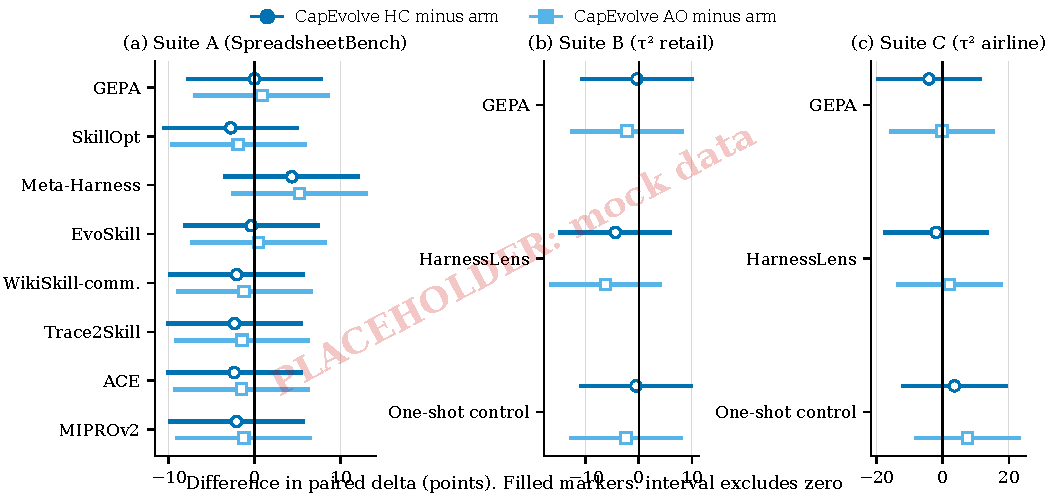
\includegraphics[width=\textwidth]{figures/fig_contrast.pdf}
\caption{Each \capevolve{} configuration against each competitor: an interval that excludes zero is a difference between the two, and one that spans zero is inconclusive. Differences are paired deltas in points with 95\% intervals (placeholder).}
\label{fig:contrast}
\end{figure*}

\begin{figure}[t]
\centering
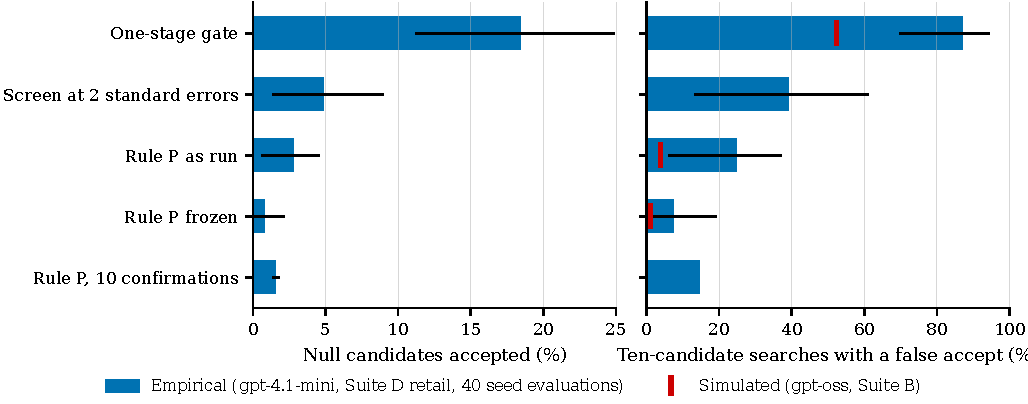
\includegraphics[width=\columnwidth]{figures/fig_nullpool.pdf}
\caption{On repeated evaluations of the unmodified seed, each gate promotes falsely in the share of searches shown, against the simulated value in red (placeholder).}
\label{fig:nullpool}
\end{figure}

\section{Additional results}
\label{app:results}


\begin{table*}[t]
\centering
\scriptsize
\setlength{\tabcolsep}{3.5pt}
\caption{Optimizer tokens in millions and wall clock per arm, summed over seeds. Non-cache-read tokens are uncached input, output and cache writes, the quantity the optimizer cap of 4M per search counts. The last token column adds cache reads, which the cap ignores. Cap used is the largest seed as a share of the cap. (placeholder)}
\label{tab:cost_tokens}
\begin{tabular}{lrrrrrr}
\toprule
Arm & Rollouts at $B^\ast$ & Non-cache-read & Cache read & Incl.\ cache read & Cap used (\%) & Wall clock (h) \\
\midrule
\multicolumn{7}{l}{\textit{Suite A, SpreadsheetBench verified-400 (Gemma-4-31B-it)}} \\
\midrule
Meta-Harness & \pend{395} & \pend{5.1} & \pend{63.9} & \pend{69.0} & \pend{51} & \pend{6.4} \\
EvoSkill & \pend{393} & \pend{3.4} & \pend{36.7} & \pend{40.1} & \pend{34} & \pend{14.3} \\
GEPA & \pend{397} & \pend{2.2} & \pend{4.1} & \pend{6.4} & \pend{22} & \pend{22.5} \\
Trace2Skill & \pend{388} & \pend{5.5} & \pend{6.6} & \pend{12.1} & \pend{55} & \pend{24.4} \\
MIPROv2 & \pend{399} & \pend{3.7} & \pend{0.8} & \pend{4.5} & \pend{37} & \pend{22.4} \\
ACE & \pend{396} & \pend{5.2} & \pend{5.4} & \pend{10.7} & \pend{52} & \pend{27.8} \\
WikiSkill (community) & \pend{393} & \pend{2.2} & \pend{3.4} & \pend{5.6} & \pend{22} & \pend{28.3} \\
SkillOpt & \pend{393} & \pend{3.9} & \pend{0.8} & \pend{4.7} & \pend{39} & \pend{19.6} \\
CapEvolve HC & \pend{394} & \pend{4.3} & \pend{78.6} & \pend{82.9} & \pend{43} & \pend{24.1} \\
CapEvolve AO & \pend{386} & \pend{7.2} & \pend{73.6} & \pend{80.8} & \pend{72} & \pend{16.7} \\
CapEvolve HC, stock gate \textit{(exploratory)} & \pend{396} & \pend{6.2} & \pend{96.4} & \pend{102.6} & \pend{62} & \pend{9.1} \\
\midrule
\multicolumn{7}{l}{\textit{Suite B, $\tau^2$ retail, sealed test-40 (gpt-oss-120b)}} \\
\midrule
One-shot control & \pend{10} & \pend{0.6} & \pend{2.1} & \pend{2.7} & \pend{6} & \pend{0.8} \\
GEPA & \pend{338} & \pend{3.0} & \pend{3.5} & \pend{6.5} & \pend{30} & \pend{18.1} \\
HarnessLens & \pend{336} & \pend{4.6} & \pend{6.7} & \pend{11.3} & \pend{46} & \pend{11.2} \\
CapEvolve HC & \pend{342} & \pend{7.9} & \pend{118.4} & \pend{126.3} & \pend{79} & \pend{15.6} \\
CapEvolve AO & \pend{350} & \pend{3.7} & \pend{109.7} & \pend{113.4} & \pend{37} & \pend{10.9} \\
\midrule
\multicolumn{7}{l}{\textit{Suite C, $\tau^2$ airline, official test-20 (development-exposed)}} \\
\midrule
One-shot control & \pend{10} & \pend{0.6} & \pend{6.8} & \pend{7.4} & \pend{6} & \pend{1.0} \\
HarnessLens & \pend{241} & \pend{1.9} & \pend{3.2} & \pend{5.1} & \pend{19} & \pend{7.4} \\
GEPA & \pend{245} & \pend{5.1} & \pend{3.5} & \pend{8.5} & \pend{51} & \pend{13.9} \\
CapEvolve HC & \pend{245} & \pend{4.1} & \pend{107.7} & \pend{111.8} & \pend{41} & \pend{20.1} \\
CapEvolve AO & \pend{247} & \pend{4.8} & \pend{119.0} & \pend{123.8} & \pend{48} & \pend{25.4} \\
CapEvolve HC, stock gate \textit{(exploratory)} & \pend{245} & \pend{7.6} & \pend{75.9} & \pend{83.5} & \pend{76} & \pend{29.8} \\
\bottomrule
\end{tabular}
\end{table*}

\begin{table*}[t]
\centering
\scriptsize
\setlength{\tabcolsep}{3.5pt}
\caption{Promotions per search for every arm, from the candidate logs, with the mean number of candidates evaluated. A promotion is a candidate that the arm's own acceptance rule put on its lineage. CapEvolve with rule P is a deliberately conservative configuration and is expected to promote rarely, and the stock-gate rows (E12) show the other side of that trade. (placeholder)}
\label{tab:promotions}
\begin{tabular}{lcccccr}
\toprule
Arm & Seed 0 & Seed 1 & Seed 2 & Mean per search & Candidates evaluated & Promoted (\%) \\
\midrule
\multicolumn{7}{l}{\textit{Suite A, SpreadsheetBench verified-400 (Gemma-4-31B-it)}} \\
\midrule
Meta-Harness & \pend{4} & \pend{1} & \pend{3} & \pend{2.7} & \pend{12.0} & \pend{22} \\
EvoSkill & \pend{4} & \pend{6} & \pend{1} & \pend{3.7} & \pend{11.3} & \pend{32} \\
GEPA & \pend{2} & \pend{6} & \pend{7} & \pend{5.0} & \pend{9.7} & \pend{52} \\
Trace2Skill & \pend{5} & \pend{5} & \pend{1} & \pend{3.7} & \pend{9.3} & \pend{39} \\
MIPROv2 & \pend{6} & \pend{5} & \pend{2} & \pend{4.3} & \pend{9.7} & \pend{45} \\
ACE & \pend{7} & \pend{4} & \pend{5} & \pend{5.3} & \pend{10.7} & \pend{50} \\
WikiSkill (community) & \pend{5} & \pend{7} & \pend{6} & \pend{6.0} & \pend{9.3} & \pend{64} \\
SkillOpt & \pend{3} & \pend{4} & \pend{6} & \pend{4.3} & \pend{9.0} & \pend{48} \\
CapEvolve HC & \pend{3} & \pend{3} & \pend{3} & \pend{3.0} & \pend{11.3} & \pend{26} \\
CapEvolve AO & \pend{2} & \pend{2} & \pend{2} & \pend{2.0} & \pend{11.7} & \pend{17} \\
CapEvolve HC, stock gate \textit{(exploratory)} & \pend{3} & \pend{2} & \pend{7} & \pend{4.0} & \pend{11.0} & \pend{36} \\
\midrule
\multicolumn{7}{l}{\textit{Suite B, $\tau^2$ retail, sealed test-40 (gpt-oss-120b)}} \\
\midrule
One-shot control & \pend{2} & \pend{2} & \pend{1} & \pend{1.7} & \pend{8.7} & \pend{19} \\
GEPA & \pend{3} & \pend{2} & \pend{3} & \pend{2.7} & \pend{10.0} & \pend{27} \\
HarnessLens & \pend{7} & \pend{4} & \pend{4} & \pend{5.0} & \pend{8.3} & \pend{60} \\
CapEvolve HC & \pend{2} & \pend{1} & \pend{0} & \pend{1.0} & \pend{7.7} & \pend{13} \\
CapEvolve AO & \pend{3} & \pend{1} & \pend{0} & \pend{1.3} & \pend{9.7} & \pend{14} \\
\midrule
\multicolumn{7}{l}{\textit{Suite C, $\tau^2$ airline, official test-20 (development-exposed)}} \\
\midrule
One-shot control & \pend{6} & \pend{4} & \pend{3} & \pend{4.3} & \pend{8.0} & \pend{54} \\
HarnessLens & \pend{2} & \pend{7} & \pend{7} & \pend{5.3} & \pend{9.7} & \pend{55} \\
GEPA & \pend{6} & \pend{4} & \pend{7} & \pend{5.7} & \pend{10.7} & \pend{53} \\
CapEvolve HC & \pend{1} & \pend{0} & \pend{0} & \pend{0.3} & \pend{8.0} & \pend{4} \\
CapEvolve AO & \pend{0} & \pend{1} & \pend{0} & \pend{0.3} & \pend{8.7} & \pend{4} \\
CapEvolve HC, stock gate \textit{(exploratory)} & \pend{5} & \pend{4} & \pend{7} & \pend{5.3} & \pend{7.7} & \pend{70} \\
\bottomrule
\end{tabular}
\end{table*}


\begin{figure*}[t]
\centering
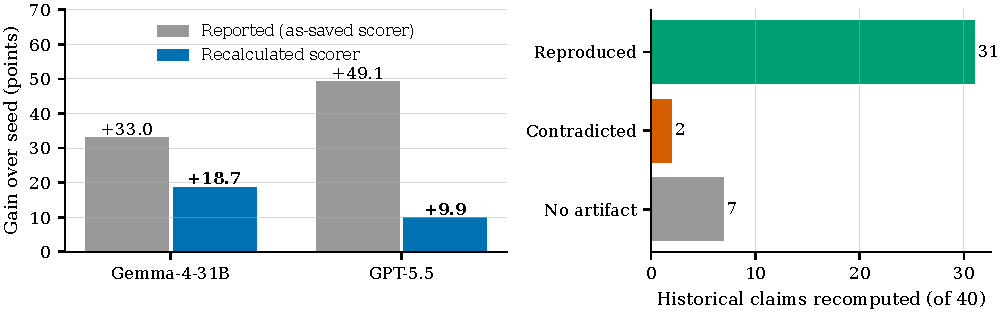
\includegraphics[width=\textwidth]{figures/fig_audit.pdf}
\caption{Recalculation removes most of the historical gain. Left: reported and recalculated gains of the two SpreadsheetBench headline runs. Right: outcome of recomputing every historical claim from archived artifacts (\texttt{audit/recomputed\_numbers.csv}).}
\label{fig:audit}
\end{figure*}

\begin{table*}[t]
\centering\scriptsize
\caption{Changes to each competitor's official code, from the per-arm deviation records (\texttt{baselines/deviations\_*.json}) and \texttt{decisions.md}. All arms share the same target rollout (Gemma-4-31B-it, 30 turns, gold-free sandbox), the same seed artifact, the same optimizer model (Claude Sonnet 5.5 through the gateway) and the same recalculated hard reward during search. ``Direction'' is our reading of how each change affects the arm relative to its published setting, not a measured effect.}
\label{tab:deviations}
\begin{tabularx}{\textwidth}{@{}l>{\raggedright\arraybackslash}X>{\raggedright\arraybackslash}X>{\raggedright\arraybackslash}p{1.9in}@{}}
\toprule
Arm & Change from the official code & Reason & Direction \\
\midrule
GEPA & Evaluator replaced by one CapEvolve rollout per example. Two text components (\texttt{prompt.md}, \texttt{task\_template.md}) updated round-robin. Every rollout counts against \texttt{max\_metric\_calls}. On Suite B the reflector is told to write only new guidance. & Same evaluator and artifact for all arms; rollout-matched budget. & Neutral for the search rule. Editing one component per proposal may slow progress on a two-file artifact. \\
SkillOpt & Rollout replaced. The two files are packed into one document. Native gold-to-agent training feedback and gold-versus-prediction reports removed. Test evaluation switched off. Optimizer temperature 0.7. & Gold-free comparison; test scored only by the campaign harness. & Lowers SkillOpt against its paper setting, because it loses oracle feedback. \\
Meta-Harness & Proposer \textsc{SKILL.md} written by us, since the upstream file is not public. Candidates are the two files, not a Python harness. Four iterations of two candidates, not about twenty. Final pick by validation mean, not Pareto frontier. Sonnet 5.5 at high effort, not Opus 4.6 at maximum. & Missing upstream file; same artifact; 600-rollout budget; matched optimizer model. & Lowers the arm: far fewer iterations and a weaker proposer. \\
EvoSkill & Base agent replaced by a CapEvolve rollout. Skills are appended to the system prompt, and skill scripts cannot run. Binary pass or fail from the recalculated score. Train pools by instruction type. Skill-only mode. & The CapEvolve agent loads only two files. & Probably lowers it, since progressive disclosure and skill tools are lost. Restarted once after the priority fault. \\
WikiSkill (community) & No official code exists, so we run the community port. Rollouts replaced. Role transport re-implemented as a tool loop on Sonnet 5.5, because the upstream transport is a Codex CLI. Skills appended to \texttt{prompt.md}. & Official code unavailable; matched optimizer model. & Unknown. The port may differ from the paper. \\
Trace2Skill & Repository's LLM-only error analyst, not the paper's agentic analyst with ground truth. README flags. A stand-in skill validator for a missing file. Uses about 200 of the 600 rollouts. & Gold-free protocol; repository omission; single-pass method. & Lowers it against the paper's strongest variant, which needs ground truth. Leaves budget unused. \\
ACE & Generator replaced by a counted CapEvolve rollout. No ground-truth mode. One reflection round, not three. Post-curator generation skipped. Output field \texttt{chain of thought} renamed to \texttt{analysis}. & Gold-free protocol; budget; the gateway returns an empty content-filter response for the original field. & Mildly lowers it (fewer rounds). The rename keeps the reflector's output usable. \\
MIPROv2 & One \texttt{dspy.Predict} whose instruction is the seed prompt. The forward pass builds \texttt{prompt.md} with demonstrations. Logging wrapper on candidate evaluation. About 400 rollouts natively. & The agent is multi-turn, not a single call; matched-checkpoint logging. & Neutral. Leaves part of the budget unused. \\
HarnessLens (Suite B) & Worker error retried once inside the budget; a second error scores zero for its internal selection only. Sandbox started with an environment allowlist. It is the only arm that streams the target. & Upstream aborts the whole stage on one worker error; isolation. & Unknown. A retry policy can lower its selection quality. \\
\bottomrule
\end{tabularx}
\end{table*}

\begin{table*}[t]
\centering
\scriptsize
\setlength{\tabcolsep}{3.5pt}
\caption{Paired delta to the seed for each search seed, in points, with the pessimistic and optimistic bounds on the mean. The pessimistic bound scores every missing cell of the arm as a loss and of the comparator as a win, and the optimistic bound does the reverse. Missing is missing over scheduled cells. (placeholder)}
\label{tab:perseed}
\begin{tabular}{lcccccr}
\toprule
Arm & Seed 0 & Seed 1 & Seed 2 & Mean $\Delta$ & Missingness bounds & Missing \\
\midrule
\multicolumn{7}{l}{\textit{Suite A, SpreadsheetBench, 70-task final set from the 912 residual pool (Gemma-4-31B-it)}} \\
\midrule
Meta-Harness & \pend{$-$2.9} & \pend{+0.4} & \pend{$-$0.9} & \pend{$-$1.1} & \pend{[$-$1.1, $-$1.1]} & \pend{0/210} \\
GEPA & \pend{+2.0} & \pend{+3.8} & \pend{+3.8} & \pend{+3.2} & \pend{[+0.8, +5.6]} & \pend{5/210} \\
EvoSkill & \pend{+4.7} & \pend{$-$0.1} & \pend{+6.1} & \pend{+3.6} & \pend{[+1.7, +5.5]} & \pend{4/210} \\
WikiSkill (community) & \pend{+5.4} & \pend{+5.0} & \pend{+5.4} & \pend{+5.3} & \pend{[+4.8, +5.8]} & \pend{1/210} \\
MIPROv2 & \pend{+5.0} & \pend{+6.1} & \pend{+4.8} & \pend{+5.3} & \pend{[+4.8, +5.8]} & \pend{1/210} \\
Trace2Skill & \pend{+4.1} & \pend{+6.0} & \pend{+6.4} & \pend{+5.5} & \pend{[+5.5, +5.5]} & \pend{0/210} \\
ACE & \pend{+4.7} & \pend{+6.8} & \pend{+5.2} & \pend{+5.6} & \pend{[+3.2, +8.0]} & \pend{5/210} \\
SkillOpt & \pend{+6.4} & \pend{+4.2} & \pend{+7.3} & \pend{+6.0} & \pend{[+5.5, +6.5]} & \pend{1/210} \\
CapEvolve as shipped, stock gate$^{\S}$ & \pend{+2.5} & \pend{+4.3} & \pend{+6.5} & \pend{+4.4} & \pend{[+0.6, +8.2]} & \pend{8/210} \\
CapEvolve HC, rule P & \pend{+1.5} & \pend{+5.9} & \pend{+2.2} & \pend{+3.2} & \pend{[+0.8, +5.6]} & \pend{5/210} \\
CapEvolve AO, rule P & \pend{+3.6} & \pend{+4.3} & \pend{+4.3} & \pend{+4.1} & \pend{[$-$0.2, +8.4]} & \pend{9/210} \\
\midrule
\multicolumn{7}{l}{\textit{Suite B, $\tau^2$ retail, sealed test-40 (gpt-oss-120b)}} \\
\midrule
One-shot control & \pend{+1.8} & \pend{+2.3} & \pend{+3.4} & \pend{+2.5} & \pend{[+2.2, +2.8]} & \pend{1/360} \\
GEPA & \pend{+1.0} & \pend{+4.1} & \pend{+2.9} & \pend{+2.7} & \pend{[+1.9, +3.5]} & \pend{3/360} \\
HarnessLens & \pend{+6.8} & \pend{+6.0} & \pend{+6.8} & \pend{+6.5} & \pend{[+6.5, +6.5]} & \pend{0/360} \\
CapEvolve HC, rule P & \pend{+4.1} & \pend{+0.0} & \pend{+4.0} & \pend{+2.7} & \pend{[+2.7, +2.7]} & \pend{0/360} \\
CapEvolve AO, rule P & \pend{+0.0} & \pend{+10.2} & \pend{+8.6} & \pend{+6.3} & \pend{[+4.9, +7.7]} & \pend{5/360} \\
\midrule
\multicolumn{7}{l}{\textit{Suite C, $\tau^2$ airline, official test-20 (development-exposed)}} \\
\midrule
One-shot control & \pend{+3.6} & \pend{+2.9} & \pend{+3.8} & \pend{+3.4} & \pend{[+2.3, +4.5]} & \pend{2/180} \\
GEPA & \pend{+1.8} & \pend{+0.2} & \pend{+0.7} & \pend{+0.9} & \pend{[$-$1.9, +3.7]} & \pend{5/180} \\
HarnessLens & \pend{+2.0} & \pend{+4.4} & \pend{+4.3} & \pend{+3.6} & \pend{[+3.6, +3.6]} & \pend{0/180} \\
CapEvolve as shipped, stock gate$^{\S}$ & \pend{+5.8} & \pend{+5.7} & \pend{+8.8} & \pend{+6.8} & \pend{[+6.2, +7.4]} & \pend{1/180} \\
CapEvolve HC, rule P & \pend{+6.4} & \pend{+3.4} & \pend{+3.5} & \pend{+4.4} & \pend{[+1.1, +7.7]} & \pend{6/180} \\
CapEvolve AO, rule P & \pend{+7.8} & \pend{+5.7} & \pend{+4.5} & \pend{+6.0} & \pend{[+6.0, +6.0]} & \pend{0/180} \\
One-shot best of $k$ & \pend{+0.3} & \pend{+0.7} & \pend{+0.5} & \pend{+0.5} & \pend{[$-$0.6, +1.6]} & \pend{2/180} \\
\bottomrule
\end{tabular}
\end{table*}


\begin{figure*}[t]
\centering
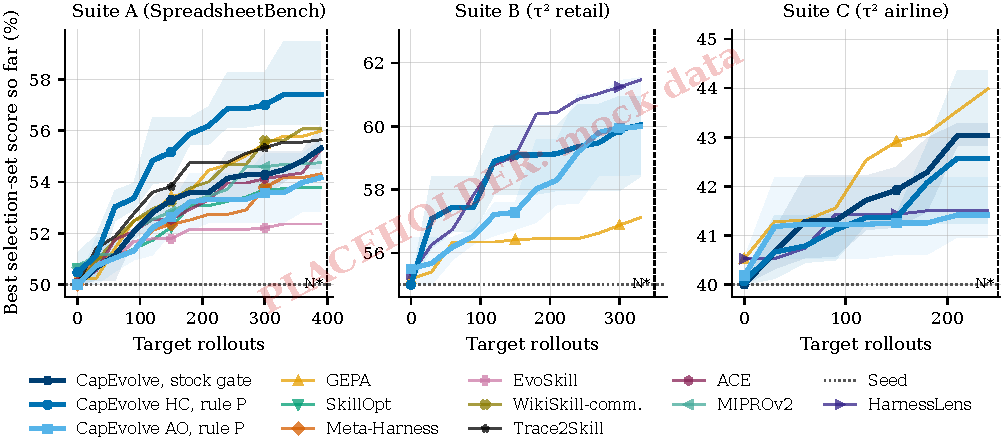
\includegraphics[width=\textwidth]{figures/fig_anytime.pdf}
\caption{Best selection-set score so far against target rollouts, with the matched checkpoint \ckpt{} dashed. The selection set is the 40 validation tasks on Suite A and the selection split on Suites B and C. Lines are averages over seeds, and bands are the minimum to maximum of the CapEvolve arms. The one-shot control has no curve because it makes one optimizer pass, and Suite A has no such control (placeholder).}
\label{fig:anytime}
\end{figure*}

\begin{figure*}[t]
\centering
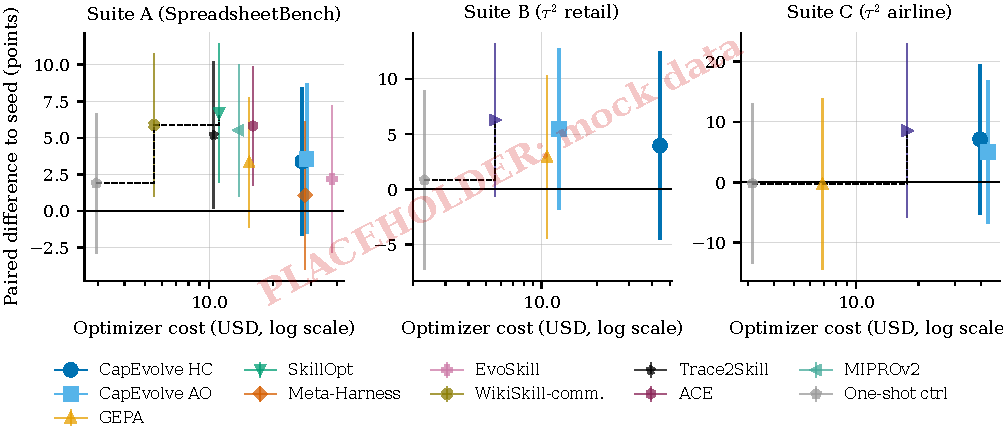
\includegraphics[width=\textwidth]{figures/fig_pareto.pdf}
\caption{Delta against optimizer cost, with the non-dominated arms joined by a dashed line. Cost is USD at Sonnet list prices on a log axis, and vertical bars are 95\% intervals (placeholder).}
\label{fig:pareto}
\end{figure*}

\begin{figure}[t]
\centering
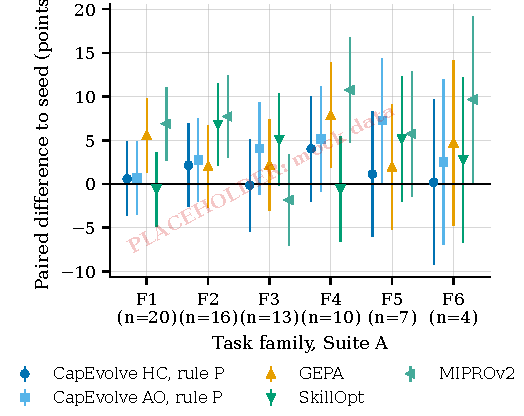
\includegraphics[width=\columnwidth]{figures/fig_families.pdf}
\caption{Delta by task family on Suite A for the main arms. Families are the cluster unit of the intervals (placeholder).}
\label{fig:families}
\end{figure}

\begin{figure*}[t]
\centering
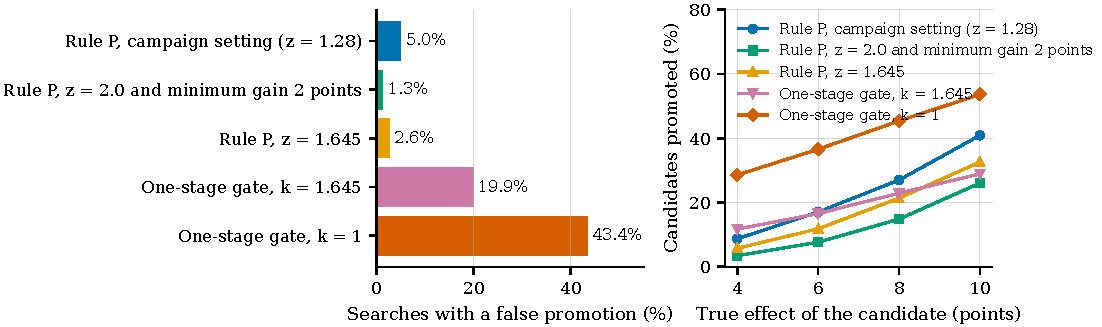
\includegraphics[width=\textwidth]{figures/fig_rulep.pdf}
\caption{Rule P promotes false candidates rarely and real ones less often than the one-stage gate. Left: share of all-null searches of six candidates with at least one false promotion. Right: share of single candidates promoted, against their true effect. The letter z is the confirmation threshold of rule P and k the threshold of the one-stage gate, both in standard errors. Source: \texttt{analysis/out/sim\_budget.md}.}
\label{fig:rulep}
\end{figure*}

\begin{figure*}[t]
\centering
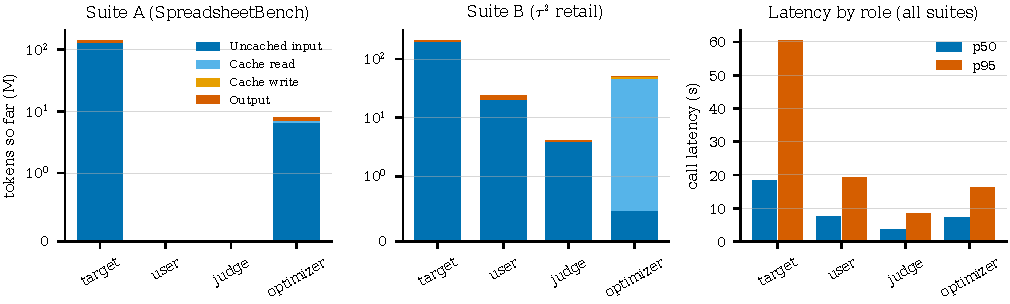
\includegraphics[width=\textwidth]{figures/fig_roles.pdf}
\caption{Target calls dominate tokens, and target calls are the slowest. Left and middle: tokens by kind for Suites A and B on a symmetric log axis. Right: call-weighted median and 95th-percentile latency per role. Main-category runs so far, in progress.}
\label{fig:roles}
\end{figure*}


\begin{table*}[t]
\centering
\scriptsize
\setlength{\tabcolsep}{3.5pt}
\caption{Campaign cost so far, from the gateway ledger (\texttt{analysis/out/metrics}). In progress: searches are still running, so every number is \prov{provisional}. Optimizer columns sum the optimizer, proposer, reflector and curator roles over seeds, in millions of tokens. The optimizer cap counts non-cache-read tokens, which are uncached input plus output plus cache writes, and applies to each search separately; the table shows the largest seed against the cap of 4M. Cache reads are listed apart and are not counted by the cap. ``0 (not started)'' means the arm is still in its baseline phase and has made no optimizer call yet; the optimizer is metered at the gateway once it runs, and the metering audit (\texttt{bypassed\_usage.csv}) found no optimizer usage outside the gateway. A double dagger would mark usage recovered from CLI transcripts. USD is a Sonnet list-price proxy for metered optimizer calls only and is a lower bound. Target tokens are uncached plus output tokens of the evaluated model. Wall is hours since launch for the longest seed. Errors count gateway calls that returned an error status, retries included. Rows count seeds that exist in the ledger.}
\label{tab:cost_so_far}
\begin{tabular}{llrrrrrrrrrr}
\toprule
Suite & Arm & Seeds & Rollouts & Opt.\ non-cache-read & Opt.\ cache read & Opt.\ incl.\ cache read & Cap used (\%) & Opt.\ USD & Target tok. (M) & Wall (h) & Errors \\
\midrule
A & CapEvolve HC & 3 & \prov{248} & \prov{0 (not started)} & \prov{0} & \prov{0} & \prov{0} & \prov{0} & \prov{14.79} & \prov{6.5} & \prov{0} \\
A & CapEvolve AO & 3 & \prov{223} & \prov{0 (not started)} & \prov{0} & \prov{0} & \prov{0} & \prov{0} & \prov{14.90} & \prov{6.4} & \prov{0} \\
A & GEPA & 3 & \prov{629} & \prov{0.34} & \prov{0.00} & \prov{0.34} & \prov{5} & \prov{1.15} & \prov{18.68} & \prov{12.8} & \prov{14} \\
A & SkillOpt & 3 & \prov{554} & \prov{2.83} & \prov{0.00} & \prov{2.83} & \prov{25} & \prov{6.59} & \prov{25.88} & \prov{12.8} & \prov{25} \\
A & Meta-Harness & 3 & \prov{589} & \prov{0.14} & \prov{0.55} & \prov{0.69} & \prov{1} & \prov{0.59} & \prov{28.82} & \prov{10.2} & \prov{15} \\
A & EvoSkill & 3 & \prov{117} & \prov{0 (not started)} & \prov{0} & \prov{0} & \prov{0} & \prov{0} & \prov{6.61} & \prov{2.7} & \prov{0} \\
A & WikiSkill & 3 & \prov{300} & \prov{0 (not started)} & \prov{0} & \prov{0} & \prov{0} & \prov{0} & \prov{17.62} & \prov{8.1} & \prov{0} \\
A & Trace2Skill & 3 & \prov{436} & \prov{6.51} & \prov{0.00} & \prov{6.51} & \prov{56} & \prov{20.27} & \prov{21.82} & \prov{12.3} & \prov{26} \\
A & ACE & 3 & \prov{74} & \prov{1.11} & \prov{0.00} & \prov{1.11} & \prov{12} & \prov{2.98} & \prov{7.90} & \prov{8.1} & \prov{0} \\
A & MIPROv2 & 3 & \prov{129} & \prov{0.54} & \prov{0.00} & \prov{0.54} & \prov{5} & \prov{1.77} & \prov{6.11} & \prov{8.1} & \prov{1} \\
\midrule
B & CapEvolve HC & 3 & \prov{441} & \prov{0.87} & \prov{9.96} & \prov{10.83} & \prov{11} & \prov{4.91} & \prov{60.75} & \prov{8.5} & \prov{58} \\
B & CapEvolve AO & 3 & \prov{369} & \prov{2.09} & \prov{30.97} & \prov{33.07} & \prov{19} & \prov{12.95} & \prov{46.78} & \prov{8.5} & \prov{54} \\
B & GEPA & 3 & \prov{483} & \prov{0.61} & \prov{0.00} & \prov{0.61} & \prov{5} & \prov{2.15} & \prov{38.53} & \prov{8.5} & \prov{42} \\
B & one-shot ctrl & 3 & \prov{394} & \prov{0.51} & \prov{6.90} & \prov{7.41} & \prov{5} & \prov{3.15} & \prov{36.02} & \prov{5.1} & \prov{21} \\
B & seed ctrl & 3 & \prov{294} & \prov{0 (no optimizer)} & \prov{0} & \prov{0} & \prov{0} & \prov{0} & \prov{33.13} & \prov{6.8} & \prov{27} \\
\midrule
C & CapEvolve HC & 3 & \prov{60} & \prov{0.32} & \prov{3.51} & \prov{3.83} & \prov{3} & \prov{1.81} & \prov{10.43} & \prov{2.8} & \prov{19} \\
C & CapEvolve AO & 3 & \prov{100} & \prov{0.66} & \prov{9.16} & \prov{9.82} & \prov{7} & \prov{3.97} & \prov{8.31} & \prov{2.8} & \prov{5} \\
C & GEPA & 3 & \prov{90} & \prov{0.08} & \prov{0.00} & \prov{0.08} & \prov{1} & \prov{0.30} & \prov{5.96} & \prov{2.8} & \prov{2} \\
C & one-shot ctrl & 3 & \prov{100} & \prov{0.33} & \prov{4.58} & \prov{4.90} & \prov{3} & \prov{2.13} & \prov{11.07} & \prov{2.8} & \prov{11} \\
C & seed ctrl & 3 & \prov{0} & \prov{0 (no optimizer)} & \prov{0} & \prov{0} & \prov{0} & \prov{0} & \prov{8.50} & \prov{2.8} & \prov{7} \\
\bottomrule
\end{tabular}
\end{table*}


\begin{table}[t]
\centering
\scriptsize
\caption{Selected historical claims and their recomputation from archived artifacts (40 claims in total).}
\label{tab:audit}
\begin{tabularx}{\columnwidth}{@{}p{0.9in}X@{}}
\toprule
Claim & Recomputation \\
\midrule
Gemma +33.0 [29.1, 36.8] & reproduces; interval is pooled over observations, task-clustered is [26.9, 39.2]; +18.7 under recalculation \\
GPT-5.5 +49.1 [45.5, 52.8] & reproduces; recalculated gain is +9.9 \\
GPT-5.5 recalculated baseline 77.5 & reproduces; 110 of 217 recalculated passes need formulas \\
no-capability control 62.9 & same run's one-iteration hill climb scores 85.6, absent from the draft \\
run excluded for different commit & 55 of 280 rollouts hit a budget error; baseline 28.9 is on 225 tasks \\
SkillsBench 55.6 to 66.7 held out & the whole delta is one trial of one task \\
SWE-bench pilot 68.0, candidate 72.0 & candidate rejected; the seed scores 63.6 and 70.5 on the same 44 tasks \\
$\tau^2$ retail 0.460 to 0.545 & arithmetic only; no per-task artifact exists \\
$\tau^2$ held-out 30.0 to 47.5 & artifact never landed; runner identity differs between docs \\
\bottomrule
\end{tabularx}
\end{table}



\end{document}
